% *********************************************************
% Digital Logic
% *********************************************************

\RequirePackage{fix-cm} % fix some latex issues see: http://texdoc.net/texmf-dist/doc/latex/base/fixltx2e.pdf
\documentclass[ twoside,openright,titlepage,numbers=noenddot,headinclude,
                footinclude=true,cleardoublepage=empty,abstractoff, 
                BCOR=5mm,fontsize=11pt,american]{scrreprt}

% *********************************************************
% Note: Make all your adjustments in here
% *********************************************************
% *********************************************************
% dl_lab-config.tex 
% *********************************************************

% *********************************************************
% Set the encoding of your files.
% *********************************************************
\PassOptionsToPackage{utf8}{inputenc}
	\usepackage{inputenc}

% *********************************************************
% Remove "drafting" below to deactivate the time-stamp on the pages
% *********************************************************
\PassOptionsToPackage{eulerchapternumbers,listings,%drafting,
  pdfspacing,floatperchapter,%linedheaders,%
  subfig,beramono,eulermath,parts}{classicthesis}
% *********************************************************
% Available options 
% (see ClassicThesis.pdf for more information):
% drafting
% parts nochapters linedheaders
% eulerchapternumbers beramono eulermath pdfspacing minionprospacing
% tocaligned dottedtoc manychapters
% listings floatperchapter subfig
% *********************************************************

% *********************************************************
% 2. Personal data and user ad-hoc commands
% *********************************************************
\newcommand{\myTitle}{Logisim-Evoluation Lab Manual\xspace}
\newcommand{\mySubtitle}{}
\newcommand{\myDegree}{}
\newcommand{\myName}{George Self\xspace}
\newcommand{\myProf}{}
\newcommand{\myOtherProf}{}
\newcommand{\mySupervisor}{}
\newcommand{\myFaculty}{}
\newcommand{\myDepartment}{Computer Information Systems\xspace}
\newcommand{\myUni}{Cochise College\xspace}
\newcommand{\myLocation}{Arizona\xspace}
\newcommand{\myTime}{July 2019\xspace}
\newcommand{\myVersion}{Edition 4.0\xspace}

% *********************************************************
% Setup, finetuning, and useful commands
% *********************************************************
\newcounter{dummy} % necessary for correct links to index, bib, etc.
\newlength{\abcd} % for ab..z string length calculation
\providecommand{\mLyX}{L\kern-.1667em\lower.25em\hbox{Y}\kern-.125emX\@}
\newcommand{\ie}{i.\,e.}
\newcommand{\Ie}{I.\,e.}
\newcommand{\eg}{e.\,g.}
\newcommand{\Eg}{E.\,g.}
\newcommand{\LE}{\textit{Logisim-Evolution} }
\newcommand{\blankpage}{ % Create a blank page at the end of the document
  \newpage
  \thispagestyle{empty}
  \mbox{}
  \newpage
  }
% The following creates a function named maxwidth that permits
% me to set a maximum width for images. If the natural width of
% the image is less than maxwidth then the image is rendered at
% its natural size, else scaled to maxwidth.
\makeatletter
\def\maxwidth#1{\ifdim\Gin@nat@width>#1 #1\else\Gin@nat@width\fi}
\makeatother

% *********************************************************
% 3. Loading some handy packages
% *********************************************************

% *********************************************************
% Packages with options that might require adjustments
% *********************************************************
\PassOptionsToPackage{american}{babel}   % change this to your language(s)
  \usepackage{babel}                  

\usepackage{csquotes}
%\PassOptionsToPackage{%
%    %backend=biber, %instead of bibtex
%  backend=bibtex8,bibencoding=ascii,%
%  language=auto,%
%  style=numeric-comp,%
%  %style=authoryear-comp, % Author 1999, 2010
%  %bibstyle=authoryear,dashed=false, % dashed: substitute rep. author with ---
%  sorting=nyt, % name, year, title
%  maxbibnames=10, % default: 3, et al.
%  %backref=true,%
%  natbib=true % natbib compatibility mode (\citep and \citet still work)
%}{biblatex}
%  \usepackage{biblatex}

\PassOptionsToPackage{fleqn}{amsmath}       % math environments and more by the AMS 
  \usepackage{amsmath}

% *********************************************************
% General useful packages
% *********************************************************
\PassOptionsToPackage{T1}{fontenc} % T2A for cyrillics
  \usepackage{fontenc}     
\usepackage{textcomp} % fix warning with missing font shapes
\renewcommand{\textuparrow}{$\uparrow$}
\renewcommand{\textdownarrow}{$\downarrow$}

\usepackage{scrhack} % fix warnings when using KOMA with listings package
\usepackage{xspace} % to get the spacing after macros right  
\usepackage{mparhack} % get marginpar right
\usepackage{fixltx2e} % fixes some LaTeX stuff --> since 2015 in the LaTeX kernel (see below)
%\usepackage[latest]{latexrelease} % will be used once available in more distributions (ISSUE #107)
\PassOptionsToPackage{printonlyused,smaller}{acronym} 
  \usepackage{acronym} % nice macros for handling all acronyms in the thesis
%\renewcommand{\bflabel}[1]{{#1}\hfill} % fix the list of acronyms --> no longer working
%\renewcommand*{\acsfont}[1]{\textsc{#1}} 
\renewcommand*{\aclabelfont}[1]{\acsfont{#1}}
\usepackage[paperheight=11in,paperwidth=8.5in]{geometry}
\usepackage{shorttoc} % generate brief version of the table of contents

% *********************************************************
% 4. Setup floats: tables, (sub)figures, and captions
% *********************************************************
\usepackage{tabularx} % better tables
\setlength{\extrarowheight}{3pt} % increase table row height
\newcommand{\tableheadline}[1]{\multicolumn{1}{c}{\spacedlowsmallcaps{#1}}}
\newcommand{\myfloatalign}{\centering} % to be used with each float for alignment
\usepackage{caption}
\captionsetup{font=small}
\usepackage{subfig}  

% *********************************************************
% 5. Setup code listings - format Verilog listings
% *********************************************************
\usepackage{listings} 
%\lstset{emph={trueIndex,root},emphstyle=\color{BlueViolet}}%\underbar} % for special keywords
\lstset{language=Verilog,%[LaTeX]Tex,
  morekeywords={PassOptionsToPackage,selectlanguage},
  keywordstyle=\color{RoyalBlue},%\bfseries,
  %basicstyle=\small\ttfamily,
  basicstyle=\ttfamily,
  identifierstyle=\color{DarkRed},
  commentstyle=\color{Green}\ttfamily,
  stringstyle=\rmfamily,
  numbers=left,
  numberstyle=\scriptsize,%\tiny
  stepnumber=2,
  numbersep=8pt,
  showstringspaces=false,
  breaklines=true,
  %frameround=ftff,
  frame=lines,
  captionpos=b,  % put captions at the bottom of the listing
  aboveskip=.75\baselineskip,
  belowskip=.75\baselineskip
  %abovecaptionskip=.75\baselineskip
  %belowcaptionskip=.75\baselineskip
  %frame=L
} 

% *********************************************************
% 6. PDFLaTeX, hyperreferences and citation backreferences
% *********************************************************

% *********************************************************
% Using PDFLaTeX
% *********************************************************
\PassOptionsToPackage{pdftex,hyperfootnotes=false,pdfpagelabels}{hyperref}
  \usepackage{hyperref}  % backref linktocpage pagebackref
\pdfcompresslevel=9
\pdfadjustspacing=1 
\PassOptionsToPackage{pdftex}{graphicx}
  \usepackage{graphicx} 
 
% *********************************************************
% Hyperreferences in the PDF output
% *********************************************************
\hypersetup{%
  %draft, % = no hyperlinking at all (useful in b/w printouts)
  colorlinks=true, linktocpage=true, pdfstartpage=3, pdfstartview=FitV,%
  % uncomment the following line if you want to have black links (e.g., for printing)
  %colorlinks=false, linktocpage=false, pdfstartpage=3, pdfstartview=FitV, pdfborder={0 0 0},%
  breaklinks=true, pdfpagemode=UseNone, pageanchor=true, pdfpagemode=UseOutlines,%
  plainpages=false, bookmarksnumbered, bookmarksopen=true, bookmarksopenlevel=1,%
  hypertexnames=true, pdfhighlight=/O,%nesting=true,%frenchlinks,%
  urlcolor=webbrown, linkcolor=RoyalBlue, citecolor=webgreen, %pagecolor=RoyalBlue,%
  %urlcolor=Black, linkcolor=Black, citecolor=Black, %pagecolor=Black,%
  pdftitle={\myTitle},%
  pdfauthor={\textcopyright\ \myName, \myUni, \myFaculty},%
  pdfsubject={},%
  pdfkeywords={},%
  pdfcreator={pdfLaTeX},%
  pdfproducer={LaTeX with hyperref and classicthesis}%
}   

% *********************************************************
% Setup autoreferences
% *********************************************************
\makeatletter
\@ifpackageloaded{babel}%
  {
    \addto\extrasamerican{%
    \renewcommand*{\figureautorefname}{Figure}%
    \renewcommand*{\tableautorefname}{Table}%
    \renewcommand*{\partautorefname}{Part}%
    \renewcommand*{\chapterautorefname}{Chapter}%
    \renewcommand*{\sectionautorefname}{Section}%
    \renewcommand*{\subsectionautorefname}{Section}%
    \renewcommand*{\subsubsectionautorefname}{Section}%
  }%
  \addto\extrasngerman{% 
    \renewcommand*{\paragraphautorefname}{Absatz}%
    \renewcommand*{\subparagraphautorefname}{Unterabsatz}%
    \renewcommand*{\footnoteautorefname}{Fu\"snote}%
    \renewcommand*{\FancyVerbLineautorefname}{Zeile}%
    \renewcommand*{\theoremautorefname}{Theorem}%
    \renewcommand*{\appendixautorefname}{Anhang}%
    \renewcommand*{\equationautorefname}{Gleichung}%        
    \renewcommand*{\itemautorefname}{Punkt}%
  }%  
  \providecommand{\subfigureautorefname}{\figureautorefname}%
}{\relax}
\makeatother

% *********************************************************
% Setup drawing environment
% *********************************************************
\usepackage[svgnames,table]{xcolor}
\usepackage{tikz}
\usetikzlibrary{circuits.logic.US,circuits.logic.IEC,circuits.ee.IEC,shapes.geometric}
\usepackage{circuitikz}
\usepackage{tikz-timing} % Timing Diagrams
\usetikztiminglibrary[new={char=Q,reset char=R}]{counters}
\usepackage{rotating} % Rotate an image
\usetikzlibrary{calc} % Do some math in tikz
\usepackage{smartdiagram} % draw ``smart'' diagrams the easy way


% *********************************************************
% This enables enumerated lists using first, second, etc.
% *********************************************************
\usepackage{moreenum}

% *********************************************************
% Used to create framed paragraphs, like "interest boxes"
% *********************************************************
\usepackage{tcolorbox}

% *********************************************************
% Used to enable strike-through text
% *********************************************************
\usepackage[normalem]{ulem}

% *********************************************************
% The Creative Commons License Package
% *********************************************************
\usepackage[type={CC},modifier={zero},version={1.0}]{doclicense}

% *********************************************************
% This package permits me to align a table column on a decimal point
% *********************************************************
\usepackage{siunitx}

% *********************************************************
% Enable certain special chars in verbatim, like underlines
% *********************************************************
\usepackage{fancyvrb}

% *********************************************************
% Used for wrapping figures
% *********************************************************
\usepackage{float}
\usepackage{wrapfig}
\restylefloat{figure}

% *********************************************************
% Used for merging cells in tables, creating a slash in a cell, 
% adjusting the width of a table to fit the text column
% *********************************************************
\usepackage{multicol}
\usepackage{multirow}
\usepackage{slashbox}
\usepackage{adjustbox}

% *********************************************************
% Permit URLs to line-break at any letter or a slash
% *********************************************************
\usepackage{url}
\renewcommand{\UrlBreaks}{\do\/\do\a\do\b\do\c\do\d\do\e\do\f\do\g\do\h\do\i\do\j\do\k\do\l\do\m\do\n\do\o\do\p\do\q\do\r\do\s\do\t\do\u\do\v\do\w\do\x\do\y\do\z\do\A\do\B\do\C\do\D\do\E\do\F\do\G\do\H\do\I\do\J\do\K\do\L\do\M\do\N\do\O\do\P\do\Q\do\R\do\S\do\T\do\U\do\V\do\W\do\X\do\Y\do\Z}

% *********************************************************
% Generate  lipsum
% *********************************************************
\usepackage{lipsum}

% *********************************************************
% Give myself some enumerate options
% *********************************************************
\usepackage{enumitem}

% *********************************************************
% I used this to just find the width of a line in cm (so I can create
% appropriately sized graphics). Load the package here and then copy the
% other line in a separate paragraph where you need the size displayed.
% *********************************************************
\usepackage{layouts}
%textwidth in cm: \printinunitsof{cm}\prntlen{\textwidth}

% *********************************************************
% 7. Last calls before the bar closes
% *********************************************************

% *********************************************************
% Development Stuff
% *********************************************************
\listfiles
%\PassOptionsToPackage{l2tabu,orthodox,abort}{nag}
%   \usepackage{nag}
%\PassOptionsToPackage{warning, all}{onlyamsmath}
%   \usepackage{onlyamsmath}

% *********************************************************
% Last, but not least...
% *********************************************************
\usepackage{classicthesis} 



% *********************************************************
% Hyphenation
% *********************************************************
%\hyphenation{put special hyphenation here}

% *********************************************************
% Begin Document
% *********************************************************
\begin{document}
\frenchspacing
\raggedbottom
\selectlanguage{american} 
\pagenumbering{roman}
\pagestyle{plain}
% *********************************************************
% Frontmatter
% *********************************************************
%*******************************************************
% Titlepage
%*******************************************************
\begin{titlepage}
% Original Title Page code follows...
    % if you want the titlepage to be centered, uncomment and fine-tune the line below (KOMA classes environment)
    \begin{addmargin}[-1cm]{-3cm}
    \begin{center}
        \large  

        \hfill

        \vfill

        \begingroup
            \color{Maroon}\spacedallcaps{\myTitle} \\ \bigskip
        \endgroup

        \spacedlowsmallcaps{\myName}

        \vfill

%        \includegraphics[width=6cm]{gfx/TFZsuperellipse_bw} \\ \medskip

%        \mySubtitle \\ \medskip   
        %\myDegree \\
        %\myDepartment \\                            
        %\myFaculty \\
        %\myUni \\ \bigskip

        \myTime\ -- \myVersion

        \vfill                      

    \end{center}  
  \end{addmargin}       
\end{titlepage}     % >>>>> Include <<<<<
\thispagestyle{empty}

\hfill

\vfill

\noindent\myName: \emph{\myTitle,} \mySubtitle %\myDegree, 
%\textcopyright\ \myTime

\doclicenseThis

%\bigskip
%
%\noindent\spacedlowsmallcaps{Supervisors}: \\
%\myProf \\
%\myOtherProf \\ 
%\mySupervisor
%
%\medskip
%
%\noindent\spacedlowsmallcaps{Location}: \\
%\myLocation
%
%\medskip
%
%\noindent\spacedlowsmallcaps{Time Frame}: \\
%\myTime
  % >>>>> Include <<<<<
%*****************************************
\chapter*{Preface}\label{preface}
%*****************************************

I have taught CIS 221, \textit{Digital Logic}, for Cochise College since about 2003 and enjoy working with students on this topic. From the start, I wanted students to work with labs as part of our studies and actually design circuits to complement our theoretical instruction. As I evaluated circuit design software I had three criteria:

\begin{itemize}
  \item \textbf{\ac{OER}}. It is important to me that students use software that is available free of charge and is supported by the entire web community. 
  \item \textbf{Platform}. While most of my students use a Windows-based system, some use Macintosh and it was important to me to use software that is available for both of those platforms. As a bonus, most OER software is also available for the Linux system, though I'm not aware of any of my students who are using Linux.
  \item \textbf{Simplicity}. I wanted to use software that was easy to master so students could spend their time understanding digital logic rather than learning the arcane structures of a simulation language.
\end{itemize}

I originally wrote a number of lab exercises using \textit{Logisim}, but the creator of that software, Carl Burch, announced that he would quit developing it in 2014. Because it was published as an open source project, a group of Swiss institutes started with the \textit{Logisim} software and developed a new version that integrated several new tools, like a chronogram, and released it under the name \LE.

It is my hope that students will find these labs instructive and the labs enhance their learning of digital logic. This lab manual is written with \LaTeX\ and published under a \href{https://creativecommons.org/publicdomain/zero/1.0/}{Creative Commons Zero} license with a goal that other instructors can modify it to meet their own needs. The source code can be found at \href{https://github.com/grself/CIS221_Lab_Manual}{my personal GITHUB page} and I always welcome comments that will help me improve this manual.

\bigskip
\begin{flushright}
  \textemdash  George Self
\end{flushright}


   % >>>>> Include <<<<<
\pagestyle{scrheadings}              % >>>>> Include <<<<<
\cleardoublepage%*******************************************************
% Brief Table of Contents
%*******************************************************
%\phantomsection
\refstepcounter{dummy}
%\pdfbookmark[1]{\briefcontentsname}{brieftableofcontents}
%\setcounter{tocdepth}{0} % <-- 2 includes up to subsections in the ToC
%\setcounter{secnumdepth}{0} % <-- 3 numbers up to subsubsections
%\manualmark
%\markboth{\spacedlowsmallcaps{\contentsname}}{\spacedlowsmallcaps{\contentsname}}
\shorttoc{Brief Contents}{0} % Only Chapter Headings 

%*******************************************************
% Table of Contents
%*******************************************************
%\phantomsection
\refstepcounter{dummy}
\pdfbookmark[1]{\contentsname}{tableofcontents}
\setcounter{tocdepth}{2} % <-- 2 includes up to subsections in the ToC
\setcounter{secnumdepth}{3} % <-- 3 numbers up to subsubsections
\manualmark
\markboth{\spacedlowsmallcaps{\contentsname}}{\spacedlowsmallcaps{\contentsname}}
\tableofcontents 
\automark[section]{chapter}
\renewcommand{\chaptermark}[1]{\markboth{\spacedlowsmallcaps{#1}}{\spacedlowsmallcaps{#1}}}
\renewcommand{\sectionmark}[1]{\markright{\thesection\enspace\spacedlowsmallcaps{#1}}}
%*******************************************************
% List of Figures and of the Tables
%*******************************************************
\clearpage

\begingroup 
    \let\clearpage\relax
    \let\cleardoublepage\relax
    \let\cleardoublepage\relax
    %*******************************************************
    % List of Figures
    %*******************************************************    
    %\phantomsection 
    \refstepcounter{dummy}
    \addcontentsline{toc}{chapter}{\listfigurename}
    \pdfbookmark[1]{\listfigurename}{lof}
    \listoffigures

    \vspace{8ex}

    %*******************************************************
    % List of Tables
    %*******************************************************
    %\phantomsection 
    \refstepcounter{dummy}
    \addcontentsline{toc}{chapter}{\listtablename}
    \pdfbookmark[1]{\listtablename}{lot}
    \listoftables
        
    \vspace{8ex}
%   \newpage
    
    %*******************************************************
    % List of Listings
    %*******************************************************      
      %\phantomsection 
    \refstepcounter{dummy}
    \addcontentsline{toc}{chapter}{\lstlistlistingname}
    \pdfbookmark[1]{\lstlistlistingname}{lol}
    \lstlistoflistings 

    \vspace{8ex}
       
    %*******************************************************
    % Acronyms
    %*******************************************************
    %\phantomsection 
    \refstepcounter{dummy}
    \pdfbookmark[1]{Acronyms}{acronyms}
    \markboth{\spacedlowsmallcaps{Acronyms}}{\spacedlowsmallcaps{Acronyms}}
    \chapter*{Acronyms}
    % Notes: alphabitize this list as you create it.
    % Accronyms in this list are not printed unless they show up in the text somewhere
    \begin{acronym}[UMLX]
        \acro{ALU}{Arithmetic Logic Unit}
        \acro{ASCII}{American Standard Code for Information Interchange}
        \acro{ASIC}{Application-Specific Integrated Circuit}
        \acro{BCD}{Binary Coded Decimal}
        \acro{BDD}{Binary Decision Diagram}
        \acro{BIOS}{Basic Input/Output System}
        \acro{BLIF}{Berkeley Logic Interchange Format}
        \acro{CAT}{Computer-Aided Tools}
        \acro{CISC}{Complex Instruction Set Computer}
        \acro{CPU}{Central Processing Unit}
        \acro{DRAM}{Dynamic Random Access Memory}
        \acro{DUT}{Device Under Test}
        \acro{EBCDIC}{Extended Binary Coded Decimal Interchange Code}
        \acro{EDA}{Electronic Design Automation}
        \acro{FSM}{Finite State Machine}
        \acro{HDL}{Hardware Description Language}
        \acro{IC}{Integrated Circuit}
        \acro{IEEE}{Institute of Electrical and Electronics Engineers}
        \acro{KARMA}{KARnaugh MAp simplifier}
        \acro{LED}{Light Emitting Diode}
        \acro{LSB}{Least Significant Bit}
        \acro{LSN}{Least Significant Nibble}
        \acro{MSB}{Most Significant Bit}
        \acro{MSN}{Most Significant Nibble}
        \acro{NaN}{Not a Number}
        \acro{OER}{Open Educational Resource}
        \acro{PLA}{Programmable Logic Array}
        \acro{PCB}{Printed Circuit Board}
        \acro{POS}{Product of Sums}
        \acro{PROM}{Programmable Read-Only Memory}
        \acro{RAM}{Random Access Memory}
        \acro{RISC}{Reduced Instruction Set Computer}
        \acro{ROM}{Read Only Memory}
        \acro{RPM}{Rotations Per Minute}
        \acro{RTL}{Register Transfer Language}
        \acro{SECDED}{Single Error Correction, Double Error Detection}
        \acro{SOP}{Sum of Products}
        \acro{SDRAM}{Synchronized Dynamic Random Access Memory}
        \acro{SRAM}{Static Random Access Memory}
        \acro{TTL}{Transistor-Transistor Logic}
        \acro{USB}{Universal Synchronous Bus}
        \acro{VHDL}{VHSIC Hardware Descriptive Language}
        \acro{VHSIC}{Very High Speed Integrated Circuit}
        \acro{VLIW}{Very Long Instruction Word}
    \end{acronym}                     
\endgroup
  % >>>>> Include <<<<<

% *********************************************************
% Part 1: Introduction
% *********************************************************
\cleardoublepage\pagenumbering{arabic}
%\setcounter{page}{90}
% use \cleardoublepage here to avoid problems with pdfbookmark
\cleardoublepage  %  >>>>> Include <<<<<
\ctparttext{\LE is used to create and test simulations of digital circuits. This part of the lab manual includes only one lab designed to introduce \LE and teach the fundamentals of using this application.}
\part{Introduction To Logisim-Evolution}
%\printinunitsof{cm}\prntlen{\textwidth} % Print the width of the text line
%********************************************
% Lab 01: Introduction to Logisim-evolution
%********************************************
\chapter{Introduction To Logisim-evolution}\label{intro}

%********************************************

% Section: Introduction
%********************************************

\section{Purpose}

This lab introduces the \LE logic simulator, which is used for all lab exercises in this manual. 

%********************************************
% Section: Procedure
%********************************************

\section{Procedure}

\subsection{Installation}

\LE is a Java application, so a Java runtime environment will need to be installed before using the application. Many students who are taking a digital logic class already have a Java runtime on their computer and can skip this step, but those who do not will need to install the Java runtime. That process is not covered in this manual but information about installing the Java runtime environment is available at \url{http://www.oracle.com/technetwork/java/javase/downloads/index.html}. It can be confusing to know which version of Java to download but students working on the labs in this manual only need the runtime, called \textit{JRE} on the website. Students who are also in programming classes will likely already have the runtime as part of the Java Developer's Kit (JDK). It can be tricky testing the Java installation since the Chrome, Firefox, and Edge browsers will not run Java apps, but students can open a command prompt and enter \lstinline|java -version| to see what version of Java their computers are running, if any.

\LE (\url{https://github.com/reds-heig/logisim-evolution}) is available as a free download. Visit the website and about halfway down the page find a section named ``Running logisim-evolution.'' Click the ``here'' link at the end of the first sentence in that section. 

Since the \LE file is a Java application, it does not need to be installed like most software. To start \LE, double-click the \LE shortcut. That will start Java and then run the \LE application. Also, \LE will not need to be uninstalled when it is no longer needed since it is not actually installed, the \LE file can simply be deleted.

\subsection{Beginner's Tutorial}

\LE comes with a beginner's tutorial available in \textsc{Help -> Tutorial}. That tutorial only takes a few minutes and introduces students to the major components of the application. Students should complete that tutorial before starting this lab.

\subsection{Logisim-evolution Workspace}

Start \LE by double-clicking its icon. The initial \LE window will be similar to Figure \ref{fig:intro-01}.

\begin{figure}[H]
	\centering
	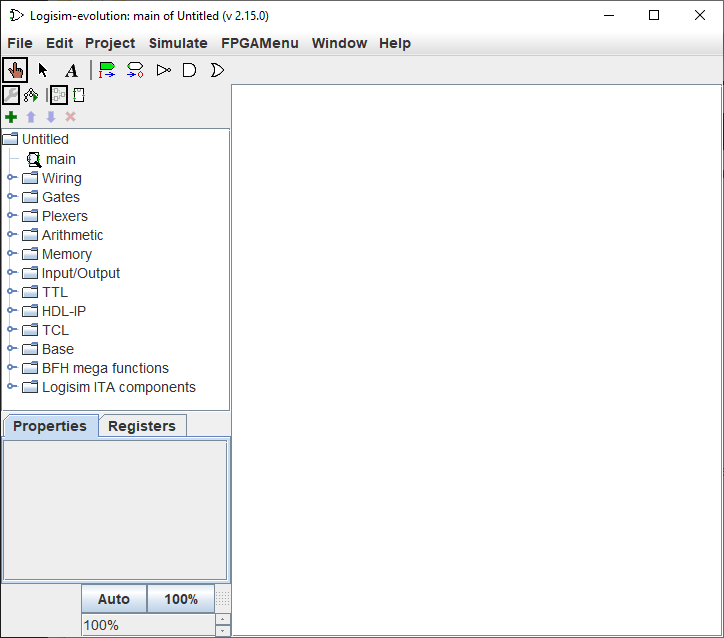
\includegraphics[width=\maxwidth{.95\linewidth}]{gfx/intro-01}
	\caption{Logisim-evolution Initial Screen}
	\label{fig:intro-01}
\end{figure}

The \LE space is divided into several areas. Along the top is a text menu that includes the types of selections found in most programs. For example, the ``File'' menu includes items like ``Save'' and ``Exit.'' The ``Edit'' menu includes an ``Undo'' option that is useful. In later labs, the various options under ``Project'' and ``Simulate'' will be described and used. Items in the ``FPGAMenu'' are beyond the scope of this class and will not be used. Of particular importance at this point is ``Library Reference'' in the ``Help'' menu. It contains information about every logical device available in \LE and is very useful while using those components in new circuits. 

Under the menu bar is the Toolbar, which is a row of eight buttons that are the most commonly used tools in \LE: 

\begin{itemize}
	\item \textbf{Pointing Finger}: Used to ``poke'' and change input values while the simulator is running. 
	\item \textbf{Arrow}: Used to select components or wires in order to modify, move, or delete them. 
	\item \textbf{A}: Activates the Text tool so text information can be added to the circuit. 
	\item \textbf{Green Input Port}: Creates an input port for a circuit. 
	\item \textbf{White Output Port}: Creates an output port for a circuit. 
	\item \textbf{NOT Gate}: Creates a NOT gate. 
	\item \textbf{AND Gate}: Creates an AND gate. 
	\item \textbf{OR Gate}: Creates an OR gate. 
\end{itemize}

The Explorer Pane is on the left side of the workspace and contains a folder list. The folders contain ``libraries'' of components organized in a logical manner. For example, the ``Gates'' folder contains various gates (AND, OR, XOR, etc.) that can be used in a circuit. The four icons across the top of the Explorer Pane are used for advanced operations and will be covered as they are needed. 

The Properties panel on the lower left side of the screen is where the properties for any selected component can be read and set. For example, the number of inputs for an AND gate can be set to a specific number.

The drawing canvas is the largest part of the screen. It is where circuits are constructed and simulated. 

\subsection{Simple Multiplexer}

\marginpar{Do not be concerned with the exact placement of components on the drawing canvas. They can be rearranged as the build progresses.}A multiplexer is used to select which of two or more inputs will be connected to a single output. For this lab, a simple two-input, one-bit multiplexer will be built. It is understood that students will not know the significance of a multiplexer at this point in the class, but the purpose of this lab is to use \LE to build a simple circuit and a multiplexer serves that purpose well. 

Start by clicking the \textit{And} button on the toolbar and placing two \texttt{AND} gates on the canvas. The canvas should resemble Figure \ref{fig:intro-02}

\begin{figure}[H]
	\centering
	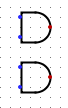
\includegraphics[width=\maxwidth{.95\linewidth}]{gfx/intro-02}
	\caption{Two AND Gates}
	\label{fig:intro-02}
\end{figure}

Click one of the AND gates to select it and observe the various properties available for that gate, as seen in Figure \ref{fig:intro-03}. The default values do not need to be changed for this circuit; however, all circuits in this manual use the ``Narrow'' gate size in order to make the circuit fit the screen better. The other properties will be explained as they are needed.

\begin{figure}[H]
	\centering
	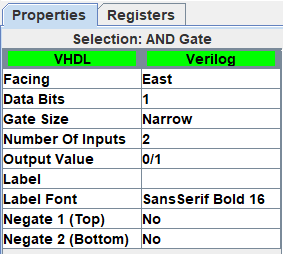
\includegraphics[width=\maxwidth{.95\linewidth}]{gfx/intro-03}
	\caption{AND Gate Properties}
	\label{fig:intro-03}
\end{figure}

The outputs of the two \texttt{AND} gates need to be combined with an \texttt{OR} gate. Add an \texttt{OR} gate as illustrated in Figure \ref{fig:intro-04}.

\begin{figure}[H]
	\centering
	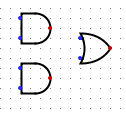
\includegraphics[width=\maxwidth{.95\linewidth}]{gfx/intro-04}
	\caption{OR Gate Added to Circuit}
	\label{fig:intro-04}
\end{figure}

The top input for the first \texttt{AND} gate needs two \texttt{NOT} gates (inverters) so the two \texttt{AND} gates can function as on/off switches. This is a rather common digital logic construct and when the circuit is complete it will become clear how the switching function works.

\begin{figure}[H]
	\centering
	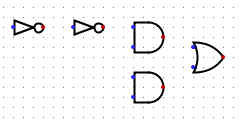
\includegraphics[width=\maxwidth{.95\linewidth}]{gfx/intro-05}
	\caption{Two NOT Gates Added to Circuit}
	\label{fig:intro-05}
\end{figure}

All inputs and outputs need to be added as in Figure \ref{fig:intro-06}. Note: inputs are square and outputs are round. The \textit{Label} property for each input and output should be specified as in the figure. The pins are labeled according to their function in the circuit. Pin \textit{Sel} carries a signal that selects which input to connect to the output, pins \textit{In1} and \textit{In2} are the two inputs, and pin \textit{Out1} is the output. Note: output pins display a blue-colored \textsf{X} until they are actually wired to some device like the \texttt{OR} gate in the illustration.
 
\begin{figure}[H]
	\centering
	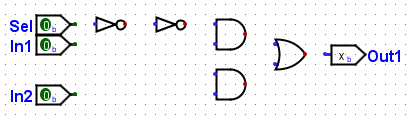
\includegraphics[width=\maxwidth{.95\linewidth}]{gfx/intro-06}
	\caption{Inputs and Output Added}
	\label{fig:intro-06}
\end{figure}

Finally, connect each device with a wire by clicking on the various ports and dragging a wire to the next port. To start the wire in the middle of the two NOT gates click the wire connecting those gates and drag downward. Wires will automatically ``bend'' one time but to get two bends, like between the output of an \texttt{AND} gate and the input of the \texttt{OR} gate, click-and-drag the wire from the output of the \texttt{AND} gate to a spot a short distance in front of that same gate, then release the mouse button and then immediately click again to start a new wire that will ``bend'' to the input of the \texttt{OR} gate. Only a little practice is needed to master this wiring technique.

\begin{figure}[H]
	\centering
	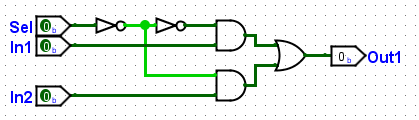
\includegraphics[width=\maxwidth{.95\linewidth}]{gfx/intro-07}
	\caption{Circuit Wiring Added}
	\label{fig:intro-07}
\end{figure}

To operate the circuit in a simulator, click the \textit{Pointing Finger} and ``poke'' the various inputs. If it is working properly, when the \textit{Sel} input is high then the value of \textit{In2} should be transmitted to the output, but when \textit{Sel} is low then the value of \textit{In1} should be transmitted to the output. This circuit is used to select one of two inputs to be transmitted to the output.

\subsection{Identifying Information}

Before finishing, add standard identification information near the top left corner of the circuit using the text tool (the \textit{A} button on the toolbar). That information should include the designer's name, the lab number and circuit name, and the date. Standard identification information for this lab would look like this:

\bigskip
% The minipage environment keeps the three lines together - no page break.
\begin{minipage}{\linewidth}
\begin{verbatim}
George Self
Lab 01: 2-Way, 1-Bit multiplexer
February 13, 2018
\end{verbatim}
\end{minipage}
\bigskip

\marginpar{The font properties in Figure \ref{fig:intro-08} have been set to bold and a large size to make the text easier to read.}Note that \textit{Logisim-evolution} will automatically center text in a new box, so text boxes will need to be aligned after they have been created. To align the text boxes, click the \textit{Arrow} tool and use it to drag the boxes to their desired location. The completed circuit should look like Figure \ref{fig:intro-08}.

\begin{figure}[H]
	\centering
	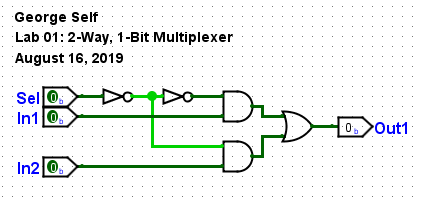
\includegraphics[width=\maxwidth{.95\linewidth}]{gfx/intro-08}
	\caption{Simple multiplexer}
	\label{fig:intro-08}
\end{figure}

\section{Deliverable}

The purpose of this lab is to install and test the \textit{Logisim-evolution} system and become comfortable creating a digital logic circuit. 

To receive a grade for this lab, create the Simple Multiplexer as defined in this lab, be sure the standard identifying information is at the top left of the circuit, and then save the file with this name: \textit{\texttt{Lab01\_Intro}}. Submit that circuit file for grading.

 

% *********************************************************
% Part 2: Theory
% *********************************************************
% use \cleardoublepage here to avoid problems with pdfbookmark
\cleardoublepage
\ctparttext{\textsc{Theory} exercises are designed to provide practice with simple logic circuits in order to both develop skill with \LE and illustrate the foundations of digital logic theory.}
\part{Theory}
%*****************************************
% Lab 02: Adder
%*****************************************
\chapter{Adder}\label{add}

\section{Purpose}

This lab builds a full 1-bit adder, but the intent is to continue to familiarize students with \LE and how basic arithmetic functions can be completed using simple gate-level logic. Additionally, this lab develops an automated testing system that will be used to test future lab submissions.

\section{Procedure}

\subsection{Half-Adder}

Open Logisim and start a new project. In \LE circuits can contain any number of sub-circuits. Subcircuits fill the same role in a physical circuit as a function or procedure fills in a software project. A new subcircuit can be added to a circuit by clicking \textsc{Project -> Add Circuit}. Name the new circuit \lstinline[columns=fixed]|Half_Adder|. Open the new subcircuit by double-clicking its name in the Explorer Pane. 

Because this is a new subcircuit, the drawing canvas is blank. A half-adder is a circuit that will add two input bits. Because it is possible to add two bits and generate a carry, the half-adder must allow for a carry out bit. Figure \ref{fig:add-01} is the circuit diagram for a half-adder.

\begin{figure}[H]
	\centering
	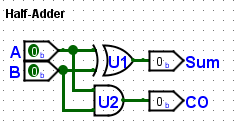
\includegraphics[width=\maxwidth{.95\linewidth}]{gfx/add-01}
	\caption{Half-Adder}
	\label{fig:add-01}
\end{figure}

This is fairly easy to build. Component \texttt{U1} is an \texttt{XOR} gate and \texttt{U2} is an \texttt{AND} gate. There are two inputs and two outputs and all of the devices should be connected as shown. To test the circuit, whenever input \textit{A} and input \textit{B} are different the \textit{Sum} should be high and when input \textit{A} and input \textit{B} are both high the \textit{CO} (Carry Out) bit should also be high.

\subsection{Full Adder}

A full adder takes two input bits and adds them, like a half-adder, but it also includes the logic necessary to input or output a carry bit so it can be cascaded with other adders. Figure \ref{fig:add-02} is the logic diagram for a full adder.

\begin{figure}[H]
	\centering
	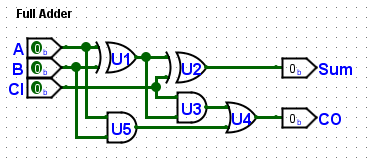
\includegraphics[width=\maxwidth{.95\linewidth}]{gfx/add-02}
	\caption{Full Adder}
	\label{fig:add-02}
\end{figure}

Create a new subcircuit named \lstinline[columns=fixed]|Full_Adder| and wire all of the components as illustrated in Figure \ref{fig:add-02}. Notice that \texttt{U1} and \texttt{U2} are \texttt{XOR} gates, \texttt{U3} and \texttt{U5} are \texttt{AND} gates, and \texttt{U4} is an \texttt{OR} gate. There are also three inputs and two outputs.

\subsection{Main Circuit}

In most \LE projects, the \lstinline[columns=fixed]|main| circuit is used to provide a nice user interface for the project. Typically, various subcircuits are dropped onto the main circuit canvas and various inputs and outputs are wired to them. A user can then test the project without worrying about the details of the subcircuits.

For this project, open the \lstinline[columns=fixed]|main| circuit by double-clicking its name in the Library panel. Click one time on the \lstinline[columns=fixed]|Full_Adder| subcircuit then move the mouse over the drawing canvas. Notice that the mouse pointer has changed into a representation of the subcircuit. Drop that subcircuit anywhere on the drawing canvas and then wire the various inputs and outputs as shown in Figure \ref{fig:add-03}.

\begin{figure}[H]
	\centering
	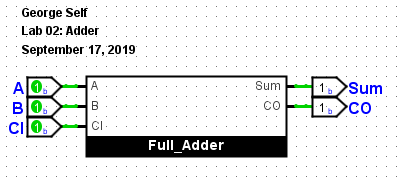
\includegraphics[width=\maxwidth{.95\linewidth}]{gfx/add-03}
	\caption{Full Adder}
	\label{fig:add-03}
\end{figure}

This circuit can be tested by using the \textit{poke} tool and entering these values. After each line, check to see that the outputs are correct.

\begin{table}[H]
	\sffamily
	\newcommand{\head}[1]{\textcolor{white}{\textbf{#1}}}		
	\begin{center}
		\rowcolors{2}{gray!10}{white} % Color every other line a light gray
		\begin{tabular}{ccccc} 
			\rowcolor{black!75}
			\multicolumn{3}{c}{\head{Inputs}} & \multicolumn{2}{c}{\head{Outputs}} \\
			A & B & CI & Sum & CO \\
			\hline
			0 & 0 & 0 & 0 & 0 \\
			0 & 1 & 0 & 1 & 0 \\
			1 & 0 & 0 & 1 & 0 \\
			1 & 1 & 0 & 0 & 1 \\
			0 & 0 & 1 & 1 & 0 \\
			0 & 1 & 1 & 0 & 1 \\
			1 & 0 & 1 & 0 & 1 \\
			1 & 1 & 1 & 1 & 1 \\
		\end{tabular}
	\end{center}
	\caption{Test Vector For Full Adder}
	\label{tab:intro-01}
\end{table}

\subsection{Automated Testing}

While it is possible to use the \textit{poke} tool and check the outputs for various input combinations, as digital logic circuits become more complex it is important to automate the testing process so no input combinations are overlooked. \LE includes a \textsc{Simulate -> Test Vector} feature that is used for automating circuit testing.

The first step in using automatic testing is to create a \textit{Test Vector} file. This is a simple \textit{.txt} file that can be created in any text processor, like \textit{Notepad}. \marginpar{Do not use a word processor to create the Test Vector since that would add unneeded codes for things like fonts and margins.} The format for a test vector is fairly simple.

\begin{itemize}
	\item Every line is a single test of the circuit, except the first line.
	\item The first line defines the various inputs and outputs being tested.
	\item Any line that starts with a hash mark (\#) is a comment and is ignored.
\end{itemize}

Following is the test vector file used to test the \lstinline[columns=fixed]|main| circuit.

\begin{Verbatim}[frame=lines,
numbers=left,
xleftmargin=10mm,
xrightmargin=10mm]
# Test vector for Adder
CI A B Sum CO
0 0 0 0 0
0 0 1 1 0
0 1 0 1 0
0 1 1 0 1
1 0 0 1 0
1 0 1 0 1
1 1 0 0 1
1 1 1 1 1
\end{Verbatim}

Following is an explanation for the \textit{Test vector for Adder} file.

\begin{description}
	\item[Line 1] This is just the title of the file. Because this line starts with a hash (\#) it is a comment and will be ignored by \LE.
	\item[Line 2] This line lists all of the inputs and outputs in the circuit under test. In this case, there are three inputs, \textit{CI}, \textit{A}, and \textit{B}, along with two outputs, \textit{Sum} and \textit{CO}. \LE is able to determine whether the pin is an input or output from its properties. 
	\item[Line 3] This line contains the first test for the circuit. This line specifies that \LE make \textit{CI}, \textit{A}, and \textit{B} equal to zero and then check to be certain that \textit{Sum} and \textit{CO} are also zero.
	\item[Other Lines] All other lines set the three input bits and specify the expected response in the output bits.
\end{description}

To start a test, click \textsc{Simulate -> Test Vector}. The window illustrated in Figure \ref{fig:add-04} opens. 

\begin{figure}[H]
	\centering
	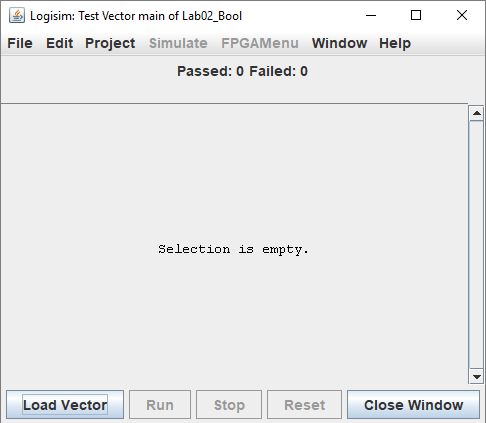
\includegraphics[width=\maxwidth{.95\linewidth}]{gfx/add-04}
	\caption{Test Vector Window}
	\label{fig:add-04}
\end{figure}

Click the \textit{Load Vector} button at the bottom of the window and load the test vector file. The test will automatically start and \LE will report the results, like in Figure \ref{fig:add-05}.

\begin{figure}[H]
	\centering
	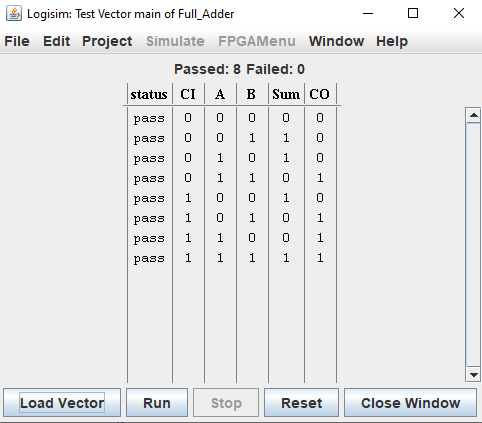
\includegraphics[width=\maxwidth{.95\linewidth}]{gfx/add-05}
	\caption{Test Completed}
	\label{fig:add-05}
\end{figure}

The test indicates all 8 lines passed and zero failed so it could be reasonably concluded that the circuit is functioning properly. Figure \ref{fig:add-06} illustrates a failed test.\marginpar{An error was intentionally added to the test vector file to generate a failed test.} The circuit designer would then need to troubleshoot to determine what went wrong with the circuit.

\begin{figure}[H]
	\centering
	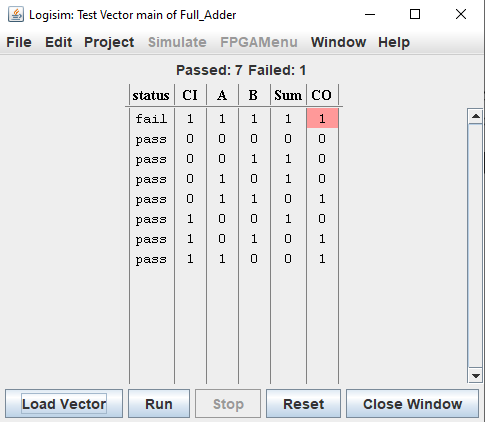
\includegraphics[width=\maxwidth{.95\linewidth}]{gfx/add-06}
	\caption{Test Failure}
	\label{fig:add-06}
\end{figure}

\textit{Note: the test vector files for all labs are made available to students so they can check their work prior to submitting them.}

\section{Deliverable}

To receive a grade for this lab, build both the half-adder and full adder and then add the full adder to the \lstinline[columns=fixed]|main|. It is important to ensure the input and output pin names are the same as in the lab instructions since a test vector will be used to check the circuit. Be sure the standard identifying information is at the top left of the \lstinline[columns=fixed]|main| circuit, similar to: 

\bigskip
% The minipage environment keeps the three lines together - no page break.
\begin{minipage}{\linewidth}
	\begin{verbatim}
	George Self
	Lab 02: Adder
	September 17, 2019
	\end{verbatim}
\end{minipage}
\bigskip

Save the file with this name: \emph{\texttt{Lab02\_Adder}} and submit that file for grading.

 
%*****************************************
% Lab 03: Arithmetic Operations
%*****************************************
\chapter{Arithmetic Operations}\label{arith}

\section{Purpose}

This lab develops an arithmetic unit that includes eight different arithmetic functions using \LE library items. This device will eventually be used as part of the \acf{ALU} in Lab \ref{alu}. This device will have two inputs, labeled \textit{A} and \textit{B}, and will output the following calculations.

\begin{enumerate}
	\item $ -1 $
	\item $ A-1 $
	\item $ A+B $
	\item $ A-B $
	\item $ AB-1 $
	\item $ AB'-1 $
	\item $ A+A $
	\item $ A+1 $
\end{enumerate}

\section{Procedure}

Start a new \LE project and create a subcircuit named \lstinline[columns=fixed]|arithmetic| that will eventually contain the entire arithmetic unit. Begin the build by adding eight devices in the subcircuit as in Figure \ref{fig:arith-01}. \textit{Notes: exact device placement is not important at this point since they can be repositioned as necessary; however, they should be in the correct order on the subcircuit. Also, all of the devices, inputs, and outputs need to be set for eight data bits in the properties panel.} 

\begin{figure}[H]
	\centering
	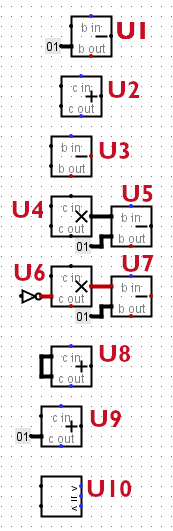
\includegraphics[width=3cm]{gfx/arith-01}
	\caption{Placing the Arithmetic Components}
	\label{fig:arith-01}
\end{figure}

Here are the devices in Figure \ref{fig:arith-01}. \textit{Note: the device numbers were added to the illustration as an aid for the following discussion; they will not be present in the \LE subcircuit.}

\begin{itemize}
	\item U1-Subtractor (\textit{Arithmetic} library). This device subtracts the bottom input from the top input on its east side and sends the result to the output on its west side.
	\item Constant (\textit{Wiring} library). Subtractor \textit{U1} is intended to supply the \textit{A-1} output and the ``01'' on its bottom input is a constant used in this calculation. It should be placed near the bottom input for subtractor \textit{U1} and its properties set for Facing: East, Data Bits: 8, Value: 0x1 (this means hexadecimal 1).
	\item U2-Adder (\textit{Arithmetic} library). This device adds the top and bottom inputs on its east side and sends the result to the output on its west side.
	\item U3-Subtractor (\textit{Arithmetic} library). This device subtracts the bottom input from the top input on its east side and sends the result to the output on its west side.
	\item U4-Multiplier (\textit{Arithmetic} library). This device multiplies the top and bottom inputs on its east side and sends the result to the output on its west side.
	\item U5-Subtractor (\textit{Arithmetic} library). This device is connected to multiplier U4 output and is intended to subtract one from its product.
	\item Constant (\textit{Wiring} library). Because subtractor U5 is designed to subtract one from the product of U4, the ``01'' on its bottom input is a constant. It should be placed near the bottom input and its properties set for Facing: East, Data Bits: 8, Value: 0x1 (this means hexadecimal 1).
	\item U6-Multiplier (\textit{Arithmetic} library). This device multiplies the top and bottom inputs on its east side and sends the result to the output on its west side.
	\item Not Gate (\textit{Gates} library). This is placed near the bottom input of multiplier U6 in order to negate that input.
	\item U7-Subtractor (\textit{Arithmetic} library). This device is connected to multiplier U6 output and is intended to subtract one from its product.
	\item Constant (\textit{Wiring} library). Because subtractor U7 is designed to subtract one from the product of U6, the ``01'' on its bottom input is a constant. It should be placed near the bottom input and its properties set for Facing: East, Data Bits: 8, Value: 0x1 (this means hexadecimal 1).	
	\item U8-Adder (\textit{Arithmetic} library). This device is designed to output the value of $ A+A $ so the two inputs on its east side are tied together. The result is sent to the output on its west side.
	\item U9-Adder (\textit{Arithmetic} library). This device adds the top and bottom inputs on its east side and sends the result to the output on its west side.
	\item Constant (\textit{Wiring} library). Adder \textit{U9} is intended to supply the \textit{A+1} output and the ``01'' on its bottom input is a constant. It should be placed near the bottom input for adder \textit{U9} and its properties set for Facing: East, Data Bits: 8, Value: 0x1 (this means hexadecimal 1).	
	\item U10-Comparator (\textit{Arithmetic} library). A comparator compares the two inputs on its east side. If the top input is greater than the bottom input then output ``$ > $'' will go high. If the top and bottom inputs are equal then output ``$ = $'' will go high. If the top input is less than the bottom input then output ``$ < $'' will go high.
\end{itemize}

The next step is to place all of the inputs and outputs. Figure \ref{fig:arith-02} shows where those items should go and the label for each item. Note: exact placement is not important since they can be repositioned. The \textit{Radix} property for each of the inputs and outputs should be set to ``Hexadecimal.'' The \textit{Data Bits} property should be set as follows.

\begin{itemize}
	\item CI: 1
	\item A: 8
	\item B: 8
	\item ArOut: 8
	\item CO: 1
	\item Cmp: 1
\end{itemize}

\begin{figure}[H]
	\centering
	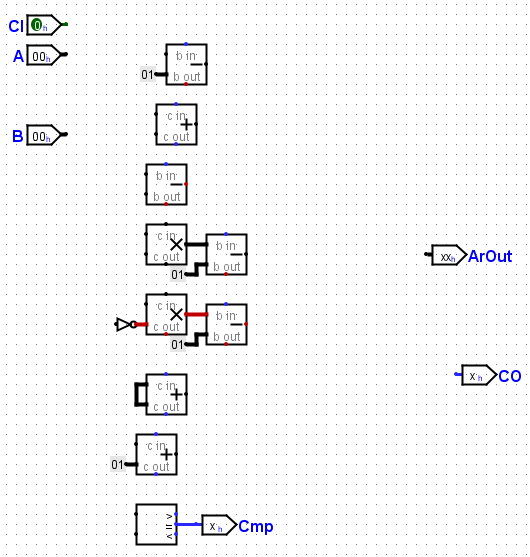
\includegraphics[width=\maxwidth{.95\linewidth}]{gfx/arith-02}
	\caption{Arithmetic Inputs and Outputs}
	\label{fig:arith-02}
\end{figure}

This circuit uses a Multiplexer (\textit{Plexers} library) to select which device's output to connect to \textit{ArOut}. A multiplexer is a digital logic workhorse that is found in many circuits, including \acp{CPU}. It is designed to switch a selected input to the output while ignoring all other input ports. In Figure \ref{fig:arith-03}, two multiplexers have been placed in the circuit. The top multiplexer will select one of eight inputs coming from the eight arithmetic devices to connect to \textit{ArOut}. The bottom multiplexer will connect the carry out signal from the selected arithmetic device to the \textit{CO} output. Also notice that the bottom multiplexer has a constant zero wired to input port zero. 

\begin{figure}[H]
	\centering
	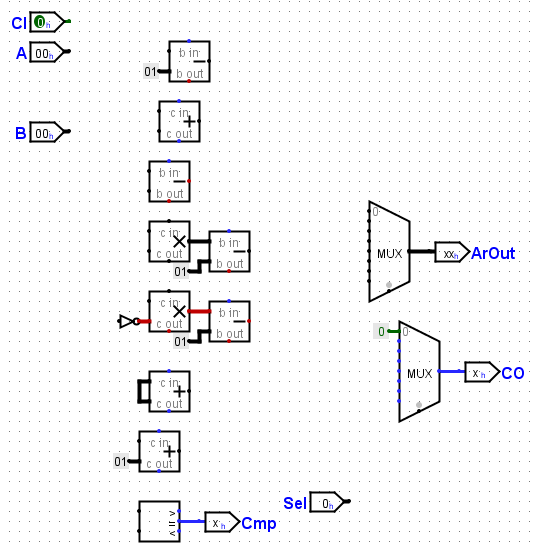
\includegraphics[width=\maxwidth{.95\linewidth}]{gfx/arith-03}
	\caption{Placing the Multiplexers}
	\label{fig:arith-03}
\end{figure}

The next step is to wire inputs \textit{A} and \textit{B} to each of the devices, as shown in Figure \ref{fig:arith-04}. Then the outputs of each device is wired to an appropriate port in the top multiplexer. This is not particularly challenging, but be careful to avoid crossed wires. 

\begin{figure}[H]
	\centering
	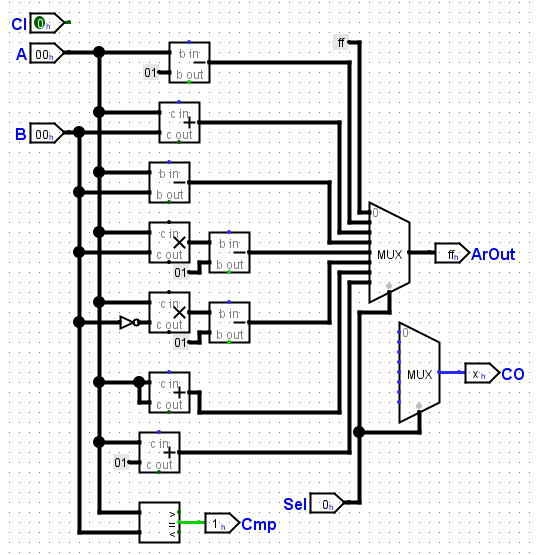
\includegraphics[width=\maxwidth{.95\linewidth}]{gfx/arith-04}
	\caption{Wiring the Data Inputs and Outputs}
	\label{fig:arith-04}
\end{figure}

Figure \ref{fig:arith-04} shows the completed subcircuit with wires connecting \textit{CI} to each device and then the devices wired to the appropriate port on the bottom multiplexer.

Notice that input zero on the top multiplexer is wired to a constant \textit{ff}. That is the two's complement of negative one so that port will always transmit negative one, as in the specification sheet. 

\begin{figure}[H]
	\centering
	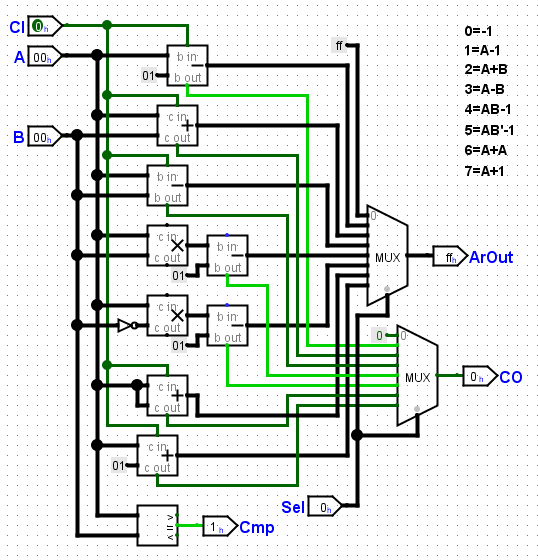
\includegraphics[width=\maxwidth{.95\linewidth}]{gfx/arith-05}
	\caption{Arithmetic Final Circuit}
	\label{fig:arith-05}
\end{figure}

Finally, the \lstinline[columns=fixed]|main| circuit is completed by dropping the \lstinline[columns=fixed]|arithmetic| subcircuit on the canvas and wiring an appropriate input or output port to each of the ports on the subcircuit. Figure \ref{fig:arith-06} illustrates the main circuit.

\begin{figure}[H]
	\centering
	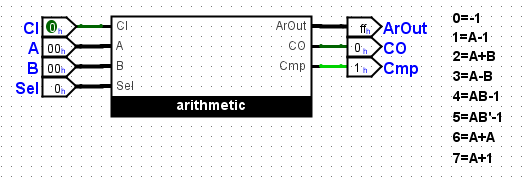
\includegraphics[width=\maxwidth{.95\linewidth}]{gfx/arith-06}
	\caption{Arithmetic Main Circuit}
	\label{fig:arith-06}
\end{figure}

This arithmetic device can be tested by entering numbers for the various inputs and checking to see if the output is correct. For example, if input \textit{A} was set to 3 and input \textit{B} were set to 4, then if \textit{Sel} is set to 2, \textit{ArOut} should be seven ($ 3+4 $). A test vector file has been provided for this lab so all of the arithmetic functions can be exercised.

As a last step, the \lstinline[columns=fixed]|main| circuit must be renamed since this circuit will be reused in Lab \ref{alu}. Click one time on the \lstinline[columns=fixed]|main| circuit to activate it and in the properties panel change its label to \lstinline[columns=fixed]|arith_main|.

\section{Deliverable}

To receive a grade for this lab, complete the circuit. Be sure the standard identifying information is at the top left of the \lstinline[columns=fixed]|arith_main| circuit, similar to: 

\bigskip
% The minipage environment keeps the three lines together - no page break.
\begin{minipage}{\linewidth}
	\begin{verbatim}
	George Self
	Lab 03: Arithmetic Operations
	September 17, 2019
	\end{verbatim}
\end{minipage}
\bigskip

Save the file with this name: \emph{\texttt{Lab03\_Arithmetic}} and submit that file for grading.


%*****************************************
% Lab 04: Logic Operations
%*****************************************
\chapter{Logic Operations}\label{logic}

\section{Purpose}

This lab develops a logic unit that includes eight different logic functions using \LE library items. This device will eventually be used as part of the \acf{ALU} in Lab \ref{alu}. This device will have two inputs, labeled \textit{A} and \textit{B}, and will output the following logic values.

\begin{enumerate}
	\item $ AB $
	\item $ (AB)' $
	\item $ A+B $
	\item $ (A+B)' $
	\item $ A Xor B $
	\item $ AB' $
	\item $ A+B' $
	\item $ A' $
\end{enumerate}

\section{Procedure}

This circuit is very similar to the arithmetic circuit developed in Lab \ref{arith}. However, the logic circuit is much simpler than the arithmetic circuit since there is not carry in/out bit and no comparator output.

To complete the lab, create a subcircuit named \lstinline[columns=fixed]|logic|. Place appropriate devices from the \textit{Gates} library in the \lstinline[columns=fixed]|logic| subcircuit. Connect each of the devices to inputs \textit{A} and \textit{B} and then wire the outputs from each device to \textit{LoOut} through a multiplexer. The exact design of the \lstinline[columns=fixed]|logic| subcircuit is left to the student.  

Drop the \lstinline[columns=fixed]|logic| subcircuit on the  \lstinline[columns=fixed]|main| circuit and wire the various inputs and outputs, as shown in Figure \ref{fig:logic-01}. 

\begin{figure}[H]
	\centering
	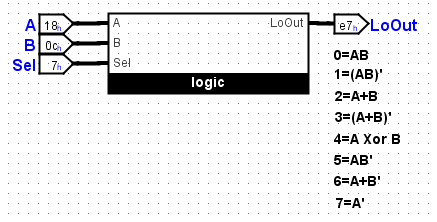
\includegraphics[width=\maxwidth{.95\linewidth}]{gfx/logic-01}
	\caption{The Main Logic Circuit}
	\label{fig:logic-01}
\end{figure}

The circuit can be tested by using the \textit{poke} tool and entering various inputs and then checking to see that the output is correct. A test vector files is also provided with the lab and that can be used to ensure the subcircuit is correct.

\section{Deliverable}

To receive a grade for this lab, complete the circuit. Be sure the standard identifying information is at the top left of the \lstinline[columns=fixed]|main| circuit, similar to: 

\bigskip
% The minipage environment keeps the three lines together - no page break.
\begin{minipage}{\linewidth}
	\begin{verbatim}
	George Self
	Lab 04: Logic Operations
	September 17, 2019
	\end{verbatim}
\end{minipage}
\bigskip

Save the file with this name: \emph{\texttt{Lab04\_Logic}} and submit that file for grading.


%********************************************
% Lab 02: Converting Boolean Logic to a Circuit
%********************************************
\chapter{Boolean Logic}

\section{Purpose}

This lab has three goals: 

\begin{itemize}
	\item Design circuits when given a Boolean expression.
	\item Create subcircuits.
	\item Create and exercise a test of the subcircuits.
\end{itemize}

\LE permits designers to work with a main circuit and any number of subcircuits. Students who have studied programming languages are familiar with ``functions'' or ``classes'' that can be designed and built one time and then reused many times whenever they are needed. \LE permits that same type of modular design by using subcircuits. 

The \LE starter for this lab includes a \lstinline[columns=fixed]|main| circuit and one subcircuit, named \lstinline[columns=fixed]|Equation_1|. The starter subcircuit is used to practice creating a circuit from a Boolean expression and then a new subcircuit is added and a second Boolean expression is used to build that circuit.

\section{Procedure}

\subsection{Subcircuit: Equation 1}

\marginpar{A magnifying glass icon is used to indicate which circuit is active on the drawing canvas.}The starter circuit includes a subcircuit named \lstinline[columns=fixed]|Equation_1|. Double-click that circuit in the Explorer Pane to activate it. The drawing canvas for this subcircuit is mostly blank except for a Boolean expression: $ (A'BC')+(AB'C')+(ABC) $. Before starting to design a circuit, it is helpful to take a minute to analyze the expression. 

\begin{itemize}
	\item There are only three variables used in the entire expression: \textit{A}, \textit{B}, and \textit{C}. Therefore, there would be three inputs into the circuit.
	\item There are three groups of variables and within each group the variables are joined with an \texttt{AND}. Therefore, the circuit must include three \texttt{AND} gates with three inputs for each gate.
	\item The three groups of variables are joined with an \texttt{OR}. Therefore, the circuit must include an \texttt{OR} gate with three inputs.
	\item While the expression does not name an output variable, it is reasonable to assume that the circuit would output a logic 1 or 0. Therefore, a one-bit output variable must be specified.
\end{itemize}

\marginpar{Do not be concerned with the exact placement of components on the drawing canvas. They can be rearranged as the build progresses.}Start by placing three inputs and an output on the drawing canvas. Inputs are indicated by a green icon with \textit{I->} on the tool bar above the drawing canvas. Click that tool and place three input pins named \textit{In1A}, \textit{In1B}, and \textit{In1C} \textemdash that means ``Input for Equation One, variable A'' and so forth. 

Outputs are indicated by a white icon with \textit{->O} found on the tool bar above the drawing canvas. Click that tool and place an output named \textit{Out1}. The circuit should look like Figure \ref{fig:02-01}.

\begin{figure}[H]
	\centering
	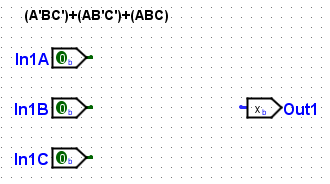
\includegraphics[width=\maxwidth{.95\linewidth}]{gfx/02-01}
	\caption{Equation 1 Inputs-Outputs}
	\label{fig:02-01}
\end{figure}

\marginpar{The gates in this manual are all ``narrow'' size. The size does not change the gate behavior but makes it easier to wire the complex circuits in later labs.}Next, the gates should be added. The \texttt{AND} gate tool can be found on the tool bar. Click that tool and place three \texttt{AND} gates on the circuit. Click each gate and in its properties panel set the \textit{Number of Inputs} to 3. 

The \texttt{OR} gate tool can be found on the tool bar. Click that tool and place one \texttt{OR} gate on the circuit. Click that gate and in its properties panel set the \textit{Number of Inputs} to 3.

The circuit should look like Figure \ref{fig:02-02}.

\begin{figure}[H]
	\centering
	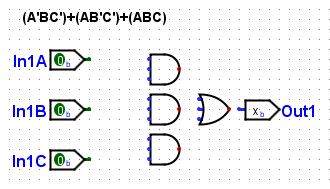
\includegraphics[width=\maxwidth{.95\linewidth}]{gfx/02-02}
	\caption{Equation 1 And-Or Gates}
	\label{fig:02-02}
\end{figure}

Next, the inputs for the \texttt{AND} gates should be set to match the Boolean expression. The top \texttt{AND} gate will match the first group of inputs, $ (A'BC') $, so inputs \textit{A} and \textit{C} should be negated. To negate those two inputs, click the \texttt{AND} gate and in the properties panel set the \textit{Negate} item for the top and bottom input to ``Yes.'' When that is done, the two inputs on the \texttt{AND} gate should include a small ``negate'' circle.

In the same way, the middle and bottom input for the second \texttt{AND} gate should also be negated. The circuit should look like Figure \ref{fig:02-03}.

\begin{figure}[H]
	\centering
	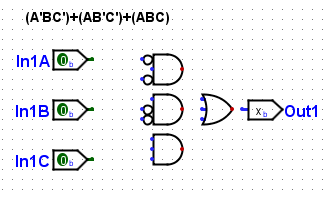
\includegraphics[width=\maxwidth{.95\linewidth}]{gfx/02-03}
	\caption{Equation 1 And Gate Inputs Set}
	\label{fig:02-03}
\end{figure}

Finally, connect all gates with wires, like Figure \ref{fig:02-04}. 

\begin{figure}[H]
	\centering
	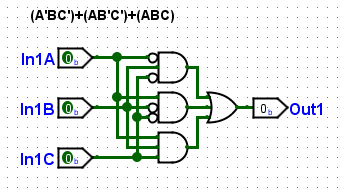
\includegraphics[width=\maxwidth{.95\linewidth}]{gfx/02-04}
	\caption{Equation 1 Circuit Completed}
	\label{fig:02-04}
\end{figure}

Test the circuit by selecting the \textit{poke} tool in the tool bar (it looks like a pointing finger) and setting various combinations of 1 and 0 on the three inputs. The output pin should go high only when the inputs are set to $ (A'BC') $, $ (AB'C') $, or $ (ABC) $.

\subsection{Subcircuit: Equation 2}

A new subcircuit can be added to a circuit by clicking \textsc{Project -> Add Circuit}. Name the new circuit \lstinline[columns=fixed]|Equation_2|. Open the new subcircuit by double-clicking its name in the Explorer Pane. 

Because this is a new subcircuit, the drawing canvas is blank. To start this subcircuit, write the equation for the circuit near the top of the drawing canvas by clicking the ``A'' button on the Toolbar and then clicking near the top of the drawing canvas and typing the following:

\[ (A'B'CD')+(A'BCD)+(AB'CD')+(ABCD') \]

It will save time to take a few minutes and analyze the expression. 

\begin{itemize}
	\item There are only four variables used in the entire expression: \textit{A}, \textit{B}, \textit{C}, and \textit{D}. Therefore, there would be four inputs into the circuit.
	\item There are four groups of variables and within each group the variables are joined with an \texttt{AND}. Therefore, the circuit must include four \texttt{AND} gates with four inputs for each gate.
	\item The four groups of variables are joined with an \texttt{OR}. Therefore, the circuit must include an \texttt{OR} gate with four inputs.
	\item While the expression does not name an output variable, it is reasonable to assume that the circuit would output a logic 1 or 0. Therefore, a one-bit output variable must be specified.
\end{itemize}

Design the subcircuit using these names for the inputs: \textit{In2A}, \textit{In2B}, \textit{In2C}, and \textit{In2D}. Also include an output named \textit{Out2}. Set the \texttt{AND} gates so the their inputs are negated properly and then wire the entire subcircuit. Finally, test the circuit to ensure the output goes high only when the four specified combinations of inputs are present.

\subsection{Main Circuit}

Make the \lstinline[columns=fixed]|main| circuit active by double-clicking its name in the Explorer Panel. Click once on the \lstinline[columns=fixed]|Equation_1| circuit and the cursor will change into an image of that circuit as it will appear on the drawing canvas. Click on the drawing canvas to drop that subcircuit. The circuit can later be moved by clicking it and dragging it to a new location. Wire the three inputs and output as shown in Figure \ref{fig:02-05}. Notice that the input/output pins do not need to be named the same as in the subcircuit; for example, the output for \lstinline[columns=fixed]|Equation_1| is labeled \textit{Out1} but it is connected to an output pin labeled \textit{True1}.

\begin{figure}[H]
	\centering
	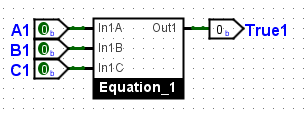
\includegraphics[width=\maxwidth{.95\linewidth}]{gfx/02-05}
	\caption{Main Circuit}
	\label{fig:02-05}
\end{figure}

Add the \lstinline[columns=fixed]|Equation_2| circuit in the same way and wire four inputs and one output to that circuit. The inputs should be labeled \textit{A2}, \textit{B2}, \textit{C2}, and \textit{D2} and the output labeled \textit{True2}.

\subsection{Testing the Circuit}

One way to test this circuit is to use the \textit{poke} tool and click various input combinations for both subcircuits. If the subcircuits are correct then the output will only go high when the correct combination is set on the inputs. However, as digital logic circuits become more complex it is important to automate the testing process so no input combinations are overlooked. \LE includes a \textsc{Simulate -> Test Vector} feature that is used for automating circuit testing.

The first step in using automatic testing is to create a \textit{Test Vector} file. This is a simple \textit{.txt} file that can be created in any text processor, like \textit{Notepad}. \marginpar{Do not use a word processor to create the Test Vector since that would add unneeded codes for things like fonts and margins.} The format for a test vector is fairly simple.

\begin{itemize}
	\item Every line is a single test of the circuit, except the first line.
	\item The first line defines the various inputs and outputs being tested.
	\item Any line that starts with a hash mark (\#) is a comment and is ignored.
\end{itemize}

Following is the test vector file used to test the \lstinline[columns=fixed]|Equation_1| subcircuit.

\begin{Verbatim}[frame=lines,
								 numbers=left,
								 xleftmargin=10mm,
								 xrightmargin=10mm]
# Test vector for Lab 2
# Equation 1
A1 B1 C1 True1
0   0  0     0
0   0  1     0
0   1  0     1
0   1  1     0
1   0  0     1
1   0  1     0
1   1  0     0
1   1  1     1
\end{Verbatim}

Following is an explanation for the \textit{Test vector for Lab 2} file.

\begin{description}
	\item[Line 1] This is just the title of the file. Because this line starts with a hash (\#) it is a comment and will be ignored by \LE.
	\item[Line 2] This is another descriptor line and is ignored by \LE.
	\item[Line 3] This line lists all of the inputs and outputs in the circuit under test. In this case, there are three inputs, \textit{A1}, \textit{B1}, and \textit{C1}, along with one output, \textit{True1}. \LE is able to determine whether the pin is an input or output from its properties. NOTE: each of the inputs and outputs in this circuit are single bits. If an input or output has more than one bit then that must be specified on this line. For example, if \textit{True1} was actually a four-bit output then that pin would be listed as \textit{True1[4]}.
	\item[Line 4] This line contains the first test for the circuit. This line specifies that \LE make \textit{A1}, \textit{B1}, and \textit{C1} equal to zero and then check to be certain that \textit{True1} is also zero.
	\item[Other Lines] All other lines set the three input bits and specify the expected response in the output bit.
\end{description}

The test vector for Equation 2 would look like this:

\begin{Verbatim}[frame=lines,
								 numbers=left,
								 xleftmargin=10mm,
								 xrightmargin=10mm]
# Test vector for Lab 2
# Equation 2
A2 B2 C2 D2 True2
0   0  0  0     0
0   0  0  1     0
0   0  1  0     1
0   0  1  1     0
0   1  0  0     0
0   1  0  1     0
0   1  1  0     0
0   1  1  1     1
1   0  0  0     0
1   0  0  1     0
1   0  1  0     1
1   0  1  1     0
1   1  0  0     0
1   1  0  1     0
1   1  1  0     1
1   1  1  1     0
\end{Verbatim}

In practice, a circuit designer would usually not create two different test vectors but would, instead, create just one file to test all parts of the circuit. Combining the \textit{Equation 1} test and the \textit{Equation 2} test is not quite as easy as appending one after the other since all input and output pins for both circuits must be specified at the top of the file. Following is the test vector for a circuit that combines \textit{Equation 1} and \textit{Equation 2}. Notice that all input and output pins are defined on line three then each line beginning with line four tests both of the equation circuits. Because only eight tests are needed to fully exercise \textit{Equation 1} but 16 are needed for Equation 2, the \textit{Equation 1} tests are repeated starting on Line 12.

\begin{Verbatim}[frame=lines,
								 numbers=left,
								 xleftmargin=10mm,
								 xrightmargin=10mm]
# Test vector for Lab 2
# Equation 1   - Equation 2
A1 B1 C1 True1   A2 B2 C2 D2 True2
0   0  0     0    0  0  0  0     0
0   0  1     0    0  0  0  1     0
0   1  0     1    0  0  1  0     1
0   1  1     0    0  0  1  1     0
1   0  0     1    0  1  0  0     0
1   0  1     0    0  1  0  1     0
1   1  0     0    0  1  1  0     0
1   1  1     1    0  1  1  1     1
0   0  0     0    1  0  0  0     0
0   0  1     0    1  0  0  1     0
0   1  0     1    1  0  1  0     1
0   1  1     0    1  0  1  1     0
1   0  0     1    1  1  0  0     0
1   0  1     0    1  1  0  1     0
1   1  0     0    1  1  1  0     1
1   1  1     1    1  1  1  1     0
\end{Verbatim}

To start a test, click \textsc{Simulate -> Test Vector}. The window illustrated in Figure \ref{fig:02-06} opens. 

\begin{figure}[H]
	\centering
	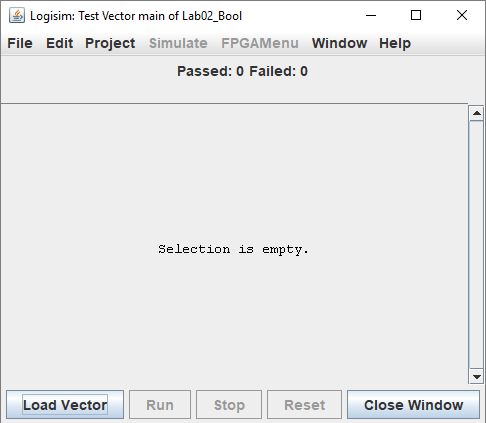
\includegraphics[width=\maxwidth{.95\linewidth}]{gfx/02-06}
	\caption{Test Vector Window}
	\label{fig:02-06}
\end{figure}

Click the \textit{Load Vector} button at the bottom of the window and load the test vector file. The test will automatically start and Logisim-evolution will report the results, like in Figure \ref{fig:02-07}.

\begin{figure}[H]
	\centering
	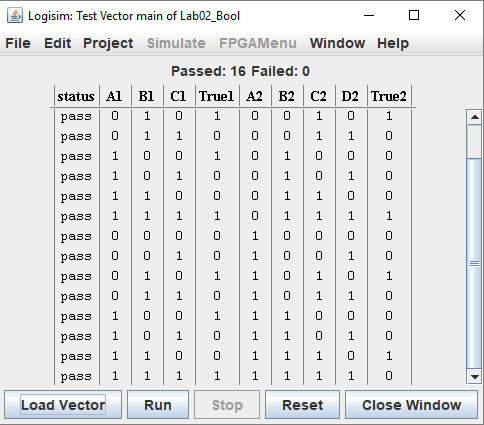
\includegraphics[width=\maxwidth{.95\linewidth}]{gfx/02-07}
	\caption{Test Completed}
	\label{fig:02-07}
\end{figure}

The test indicates all 16 lines passed and zero failed so it could be reasonably concluded that the circuits are functioning properly. Figure \ref{fig:02-08} illustrates a failed test. The circuit designer would then need to troubleshoot to determine what went wrong with the circuit.

\begin{figure}[H]
	\centering
	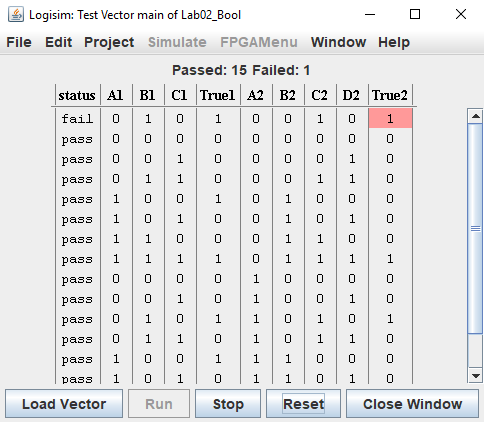
\includegraphics[width=\maxwidth{.95\linewidth}]{gfx/02-08}
	\caption{Test Failure}
	\label{fig:02-08}
\end{figure}

\section{Deliverable}

\marginpar{It is important to name all inputs and outputs as specified in the lab since they are checked with a Test Vector file that depends on those names.}To receive a grade for this lab, complete the \lstinline[columns=fixed]|main| circuit and both subcircuits. Be sure the standard identifying information is at the top left of the \lstinline[columns=fixed]|main| circuit, similar to: 

\bigskip
% The minipage environment keeps the three lines together - no page break.
\begin{minipage}{\linewidth}
	\begin{verbatim}
	George Self
	Lab 02: Boolean Equations
	February 18, 2018
	\end{verbatim}
\end{minipage}
\bigskip

Save the file with this name: \emph{\texttt{Lab02\_Bool}} and submit that file for grading.


%*****************************************
% Lab 06: PLA
%*****************************************
\chapter{Programmable Logic Array}\label{pla}

\section{Purpose}

This lab explores using a \ac{PLA} to simplify circuits that are designed for Boolean operations. A \ac{PLA} is an \ac{IC} that contains an array of \texttt{AND} and \texttt{OR} gates that can be linked in whatever way the circuit designer needs. A single \ac{PLA} can replace dozens of other gates and greatly simplify circuit design.

\section{Procedure}

\subsection{Equation One}

\begin{align}
	\label{eq:pla-01}
	(A'BC')+(AB'C')+(ABC)
\end{align}

In Lab \ref{bool} the circuit in Figure \ref{fig:pla-01} was developed to realize a Boolean expression.

\begin{figure}[H]
	\centering
	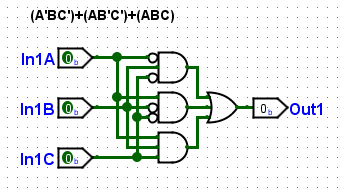
\includegraphics[width=\maxwidth{.95\linewidth}]{gfx/bool-04}
	\caption{Boolean Expression Realized}
	\label{fig:pla-01}
\end{figure}

This entire circuit can be realized in a single \ac{PLA} saving the cost of redundant \texttt{NOT/AND/OR} gates and improving the reaction time for the circuit while reducing the heat it generates.

The \LE \ac{PLA} component is a single box, as illustrated in \ref{fig:pla-02}. This \ac{PLA} has a 3-bit input attached, for inputs \textit{A}, \textit{B}, and \textit{C}, and a 1-bit output. The input is labeled \textit{ABC1} to indicate this is the input for equation one. 

\begin{figure}[H]
	\centering
	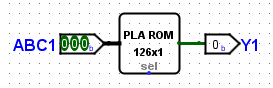
\includegraphics[width=\maxwidth{.95\linewidth}]{gfx/pla-01}
	\caption{Equation One}
	\label{fig:pla-02}
\end{figure}

Internally, a \ac{PLA} contains a matrix of \texttt{NOT/AND/OR} gates that are connected by the circuit designer. Figure \ref{fig:pla-03} illustrates the internal connections for the Equation One \ac{PLA}.

\begin{figure}[H]
	\centering
	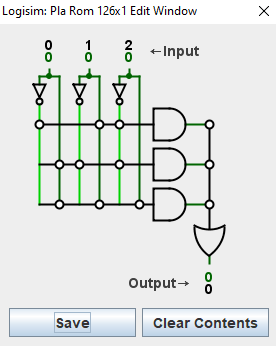
\includegraphics[width=\maxwidth{.95\linewidth}]{gfx/pla-02}
	\caption{PLA Internal Connections}
	\label{fig:pla-03}
\end{figure}

The three inputs are at the top of the \ac{PLA} and are labeled input 0, 1, and 2. Also, the values of those inputs is indicated immediately under the input number. At this time, all three are inputting a zero.

Notice that all three inputs are split and a \texttt{NOT} gate is inserted in one of the two split lines. By doing this, both \textit{A} and \textit{A'} are available on \ac{PLA} input zero. 

To the right of the grid is a column of three \texttt{AND} gates. These gates look a bit odd since there is only one input for each gate. This, though, simply represents that the \texttt{AND} gate has a variable number of inputs, depending on how the designer wired the circuit. For example, the top row has three connections to the top \texttt{AND} gate so it is a 3-input gate. The gate sizing happens automatically within the \ac{PLA} so the designer does not have to worry about it.

In the same way, there is a single \texttt{OR} gate near the bottom of the \ac{PLA}. While the diagram indicates that the \texttt{OR} gate has a single input, that gate actually has a variable input and will expand as necessary to support the circuit design. In this case, three separate rows are connected to the \texttt{OR} gate so it is a 3-input gate.

The very bottom of the \ac{PLA} is the output. It is numbered as output zero and its current value is zero.

To wire the \ac{PLA} device, the designer clicks on the wire intersections to place a connector (the small circle). Thus, row one of this device is connecting \textit{A'}, \textit{B}, and \textit{C'} to the top \texttt{AND} gate, which is then connected to the output \texttt{OR} gate.

Inspecting the connections for each row in this device should reveal that the top row is $ (A'BC') $, the second row is $ (AB'C') $ and the third row is $ (ABC) $, which are the three gates in the Boolean expression. The outputs from all three of those gates goes through an \texttt{OR} gate to the output. 

Thus, this one \ac{PLA} replaces all of the circuitry found in Figure \ref{fig:pla-01}.

Before moving on to the second equation, it will be helpful to take a look at the properties for a \ac{PLA}.

\begin{figure}[H]
	\centering
	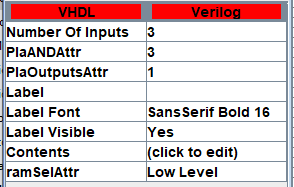
\includegraphics[width=\maxwidth{.95\linewidth}]{gfx/pla-03}
	\caption{PLA Properties}
	\label{fig:pla-04}
\end{figure}

The first property sets the number of inputs for the \ac{PLA}, the second property, \textit{PalANDAttr}, sets the number of \texttt{AND} gates and the third property, \textit{PlaOutputsAttr}, sets the number of outputs. These three properties ensure that the \ac{PLA} device can be used for many different applications. The three label properties are the same as found in most \LE components. Clicking the \textit{Contents} property will open the \ac{PLA} editor as illustrated in Figure \ref{fig:pla-03}\footnote{Important! The \LE \ac{PLA} seems to have a minor bug and the Contents editor will not always open. However, if the \textit{ramSelAttr} is clicked so its drop-down list is visible then the Contents \textit{(click to edit)} link will function properly. This is odd, but it will hopefully be corrected in a future iteration of \LE.}. Finally, the \textit{ramSelAttr} determines whether the \textit{Select} port, on the south edge of the \ac{PLA} is enabled on a high or low signal. The enable port is not used in this lab.

\subsection{Equation Two}

\begin{align}
	\label{eq:pla-02}
	(BCD')+(A'B'C)+(A'BCD')+(ABCD)
\end{align}

The subcircuit for Equation Two is very similar to that for Equation One, but the \ac{PLA} has different internal connections.

\begin{figure}[H]
	\centering
	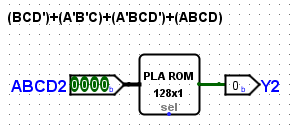
\includegraphics[width=\maxwidth{.95\linewidth}]{gfx/pla-04}
	\caption{Equation Two}
	\label{fig:pla-05}
\end{figure}

Notice that the input has four bits since the equation includes inputs \textit{A}, \textit{B}, \textit{C}, and \textit{D}. Also, the inputs and outputs include the number $ 2 $ to differentiate this subcircuit from the others.

When building this subcircuit be sure to use a \ac{PLA} device from the library instead of copy/paste from the subcircuit for Equation One. The internal connections for Equation Two are illustrated in Figure \ref{fig:pla-06}.

\begin{figure}[H]
	\centering
	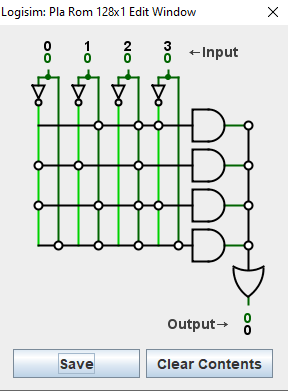
\includegraphics[width=\maxwidth{.95\linewidth}]{gfx/pla-05}
	\caption{Connections for Equation Two}
	\label{fig:pla-06}
\end{figure}

Notice that this equation includes two terms that have only three variables instead of four: (BCD') and (A'B'C). It does not cause a problem when a term in incomplete, only the variables present in the term are connected and the missing variable is ignored.

\subsection{Equation Three}

\begin{align}
	\label{eq:pla-03}
	&(A'BC')+(AB'C')+(ABC) \\
	\nonumber
	&(A'B'CD')+(A'BCD)+(AB'CD')+(ABCD')
\end{align}

The subcircuit for Equation Three is very similar to that for Equation Two, but the \ac{PLA} has different internal connections.

\begin{figure}[H]
	\centering
	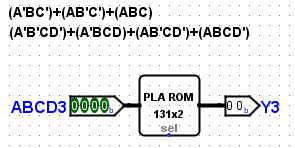
\includegraphics[width=\maxwidth{.95\linewidth}]{gfx/pla-06}
	\caption{Equation Three}
	\label{fig:pla-07}
\end{figure}

The major difference in Equation Three is that there are two outputs, so the \ac{PLA} must have two outputs specified and each equation is connected to the correct output.

\begin{figure}[H]
	\centering
	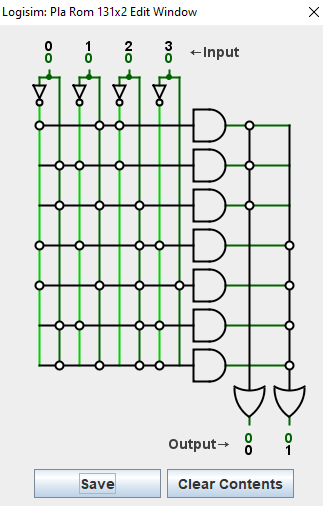
\includegraphics[width=\maxwidth{.95\linewidth}]{gfx/pla-07}
	\caption{Connections for Equation Three}
	\label{fig:pla-08}
\end{figure}

\section{Challenge}

On the \lstinline[columns=fixed]|main| circuit, wire a \ac{PLA} device using the same procedure that was used for circuits one, two, and three. That \ac{PLA} should display the correct outputs for equations \ref{eq:pla-04}.

\begin{align}
	\label{eq:pla-04}
	&(A'BC)+(ABC'D)+(A'B'CD) \\
	\nonumber
	&(BCD')+(A'B'C)+(A'BCD')+(ABCD)
\end{align}

The main circuit can be tested with the test vector provided with the lab starter circuit.

\section{Deliverable}

To receive a grade for this lab, complete the circuit. Be sure the standard identifying information is at the top left of the \lstinline[columns=fixed]|main| circuit, similar to: 

\bigskip
% The minipage environment keeps the three lines together - no page break.
\begin{minipage}{\linewidth}
	\begin{verbatim}
	George Self
	Lab 06: PLA
	September 17, 2019
	\end{verbatim}
\end{minipage}
\bigskip

Save the file with this name: \emph{\texttt{Lab06\_PLA}} and submit that file for grading.



% *********************************************************
% Part 3: Practice
% *********************************************************
% use \cleardoublepage here to avoid problems with pdfbookmark
\cleardoublepage  %  >>>>> Include <<<<<
\ctparttext{\textsc{Practice} exercises are designed to familiarize students with many aspects of both combinational and sequential digital logic circuits. This section develops devices as varied as counters, encoders, and read-only memory. It also includes a rather complex }  
\part{Practice}  
%%**************************************************************
% Lab 06: Counter
%**************************************************************
\chapter{Counters}

Counters are perhaps the most commonly-used circuits in electronic devices. They are found in virtually all electronics systems, from the simplest embedded computers to massive mainframes. Counters are designed to cycle through a specific predefined sequence of binary numbers when an input pulse is applied. Typically, counters simply count up or down from given start and end numbers, but they can be designed to produce unique output patterns for special uses. 

Counters, though, are used for more than simple counting. They can measure time so devices like alarm clocks and watches include counters. They are used as frequency dividers so a fast input frequency can be output at a slower rate. In devices with memory they are used to increment memory addresses as a program steps through some process. They can activate a series of subcircuits in sequence as part of a complex process. They are, in short, one of the most important workhorses of the digital logic world.

\section{Purpose}

This lab has two goals: 

\begin{enumerate}
	\item Develop several different common counters using \textit{D} flip-flops. Because there are two main families of counters, asynchronous and synchronous, this lab includes examples of both. 
	\item Introduce the \LE chronogram feature that generates a timing diagram as a sequential circuit functions. 
\end{enumerate}

\section{Procedure}

\subsection{Asynchronous Up Counter}

A counter is built from a series of flip-flops and where the output from each flip-flop is combined to create the counter output, trigger the next flip-flop, or both. Each flip-flop is considered a ``stage'' of the counter. A counter is triggered by a clock signal that is typically supplied by a timer with a regularly-recurring pattern of high/low levels, but it can also be triggered by an event of some sort, like the press of a button or the completion of a process.

\marginpar{In all Counter circuits in this manual flip-flop U0 provides the Least Significant Bit to the output and U3 provides the Most Significant Bit.}One of the simplest counters is illustrated in Figure \ref{fig:06-01}. This is an asynchronous four-stage up counter. A counter is is considered ``asynchronous'' if the input clock signal is applied to only the first stage and then that signal ripples through each flip-flop in turn. Thus, an asynchronous counter is frequently called a ``ripple'' counter.

\begin{figure}[H]
	\centering
	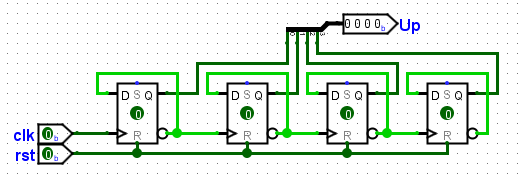
\includegraphics[width=\maxwidth{.95\linewidth}]{gfx/06-01}
	\caption{Asynchronous Up Counter}
	\label{fig:06-01}
\end{figure}

The following list describes the operation of the counter in Figure \ref{fig:06-01}. Students should open the counter circuit with \LE then use the ``poke'' tool to set the clock high then low (one complete clock cycle) as they follow the description below.

\begin{description}
	\item [Reset is Activated] All flip-flops are reset so \textit{Q} is low and \textit{Q'} is high.

	%%%%%%%%%%%%%%%
	\item [Tick 1] \textit{U0} clocked: \textit{Q0} \textuparrow \: \textemdash \: \textit{Q'0} \textdownarrow

	%%%%%%%%%%%%%%%
	\item [Tick 2] \textit{U0} clocked: \textit{Q0} \textdownarrow \: \textemdash \: \textit{Q'0} \textuparrow
	
	\hspace{14pt}\textit{U1} clocked: \textit{Q1} \textuparrow \: \textemdash \: \textit{Q'1} \textdownarrow
	
	%%%%%%%%%%%%%%%
	\item [Tick 3] \textit{U0} clocked: \textit{Q0} \textuparrow \: \textemdash \: \textit{Q'0} \textdownarrow

	%%%%%%%%%%%%%%%
	\item [Tick 4] \textit{U0} clocked: \textit{Q0} \textdownarrow \: \textemdash \: \textit{Q'0} \textuparrow

	\hspace{14pt}\textit{U1} clocked: \textit{Q1} \textdownarrow \: \textemdash \: \textit{Q'1} \textuparrow

	\hspace{14pt}\textit{U2} clocked: \textit{Q2} \textuparrow \: \textemdash \: \textit{Q'2} \textdownarrow

	%%%%%%%%%%%%%%%
	\item [Tick 5] \textit{U0} clocked: \textit{Q0} \textuparrow \: \textemdash \: \textit{Q'0} \textdownarrow

	%%%%%%%%%%%%%%%
	\item [Tick 6] \textit{U0} clocked: \textit{Q0} \textdownarrow \: \textemdash \: \textit{Q'0} \textuparrow

	\hspace{14pt}\textit{U1} clocked: \textit{Q1} \textuparrow \: \textemdash \: \textit{Q'1} \textdownarrow
	
	%%%%%%%%%%%%%%%
	\item [Tick 7] \textit{U0} clocked: \textit{Q0} \textuparrow \: \textemdash \: \textit{Q'0} \textdownarrow

	%%%%%%%%%%%%%%%
	\item [Tick 8] \textit{U0} clocked: \textit{Q0} \textdownarrow \: \textemdash \: \textit{Q'0} \textuparrow

	\hspace{14pt}\textit{U1} clocked: \textit{Q1} \textdownarrow \: \textemdash \: \textit{Q'1} \textuparrow
	
	\hspace{14pt}\textit{U2} clocked: \textit{Q2} \textdownarrow \: \textemdash \: \textit{Q'2} \textuparrow

	\hspace{14pt}\textit{U3} clocked: \textit{Q3} \textuparrow \: \textemdash \: \textit{Q'3} \textdownarrow

\end{description}

As the clock continues the counter would cycle through the binary values 1001 - 1111. The following table lists the \textit{Up} counter output as indicated by the \textit{Q} values at each tick listed above.

\begin{table}[H]
	\sffamily
	\newcommand{\head}[1]{\textcolor{white}{\textbf{#1}}}		
	\begin{center}
		\rowcolors{2}{gray!10}{white} % Color every other line a light gray
		\begin{tabular}{cc} 
			\rowcolor{black!75}
			\head{Tick} & \head{Output} \\
			Reset & 0000 \\
			1 & 0001 \\
			2 & 0010 \\
			3 & 0011 \\
			4 & 0100 \\
			5 & 0101 \\
			6 & 0110 \\
			7 & 0111 \\
			8 & 1000
		\end{tabular}
	\end{center}
	\caption{Up Counter Output}
	\label{tab0601}
\end{table}

\subsection{Asynchronous Down Counter}

The asynchronous down counter illustrated in Figure \ref{fig:06-02} is very similar to the up counter in Figure \ref{fig:06-01} except the stages are triggered from the \textit{Q} output of the preceding stage rather than \textit{Q'} and the \textit{Reset} signal is applied to the flip-flop \textit{S} input rather than \textit{R}.

\begin{figure}[H]
	\centering
	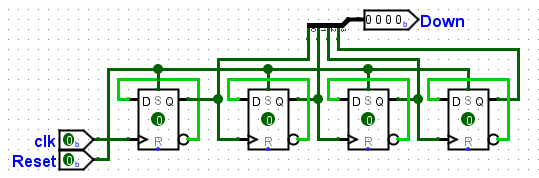
\includegraphics[width=\maxwidth{.95\linewidth}]{gfx/06-02}
	\caption{Asynchronous Down Counter}
	\label{fig:06-02}
\end{figure}

The following list describes the operation of the counter in Figure \ref{fig:06-02}. Students should open the counter circuit with \LE then use the ``poke'' tool to set the clock high then low (one complete clock cycle) as they follow the description below.

\begin{description}
	\item [Reset is activated] All flip-flops are set so \textit{Q} is high and \textit{Q'} is low.
	
	\item [Tick 1] \textit{U0} clocked: \textit{Q0} \textdownarrow \: \textemdash \: \textit{Q'0} \textuparrow

	%%%%%%%%%%%%%%%
	\item [Tick 2] \textit{U0} clocked: \textit{Q0} \textuparrow \: \textemdash \: \textit{Q'0} \textdownarrow
	
	\hspace{14pt}\textit{U1} clocked: \textit{Q1} \textdownarrow \: \textemdash \: \textit{Q'1} \textuparrow
	
	%%%%%%%%%%%%%%%
	\item [Tick 3] \textit{U0} clocked: \textit{Q0} \textdownarrow \: \textemdash \: \textit{Q'0} \textuparrow

	%%%%%%%%%%%%%%%
	\item [Tick 4] \textit{U0} clocked: \textit{Q0} \textuparrow \: \textemdash \: \textit{Q'0} \textdownarrow
	
	\hspace{14pt}\textit{U1} clocked: \textit{Q1} \textuparrow \: \textemdash \: \textit{Q'1} \textdownarrow
	
	\hspace{14pt}\textit{U2} clocked: \textit{Q2} \textdownarrow \: \textemdash \: \textit{Q'2} \textuparrow

	%%%%%%%%%%%%%%%
	\item [Tick 5] \textit{U0} clocked: \textit{Q0} \textdownarrow \: \textemdash \: \textit{Q'0} \textuparrow

	%%%%%%%%%%%%%%%	
	\item [Tick 6] \textit{U0} clocked: \textit{Q0} \textuparrow \: \textemdash \: \textit{Q'0} \textdownarrow
	
	\hspace{14pt}\textit{U1} clocked: \textit{Q1} \textdownarrow \: \textemdash \: \textit{Q'1} \textuparrow

	%%%%%%%%%%%%%%%
	\item [Tick 7] \textit{U0} clocked: \textit{Q0} \textdownarrow \: \textemdash \: \textit{Q'0} \textuparrow

	%%%%%%%%%%%%%%%
	\item [Tick 8] \textit{U0} clocked: \textit{Q0} \textuparrow \: \textemdash \: \textit{Q'0} \textdownarrow
	
	\hspace{14pt}\textit{U1} clocked: \textit{Q1} \textuparrow \: \textemdash \: \textit{Q'1} \textdownarrow
	
	\hspace{14pt}\textit{U2} clocked: \textit{Q2} \textuparrow \: \textemdash \: \textit{Q'2} \textdownarrow
	
	\hspace{14pt}\textit{U3} clocked: \textit{Q3} \textdownarrow \: \textemdash \: \textit{Q'3} \textuparrow
	
\end{description}

As the clock continues the counter would cycle through the binary values 0110 - 0000. The following table lists the \textit{Down} counter output as indicated by the \textit{Q} values at each tick listed above.

\begin{table}[H]
	\sffamily
	\newcommand{\head}[1]{\textcolor{white}{\textbf{#1}}}		
	\begin{center}
		\rowcolors{2}{gray!10}{white} % Color every other line a light gray
		\begin{tabular}{cc} 
			\rowcolor{black!75}
			\head{Tick} & \head{Output} \\
			Reset & 1111 \\
			1 & 1110 \\
			2 & 1101 \\
			3 & 1100 \\
			4 & 1011 \\
			5 & 1010 \\
			6 & 1001 \\
			7 & 1000 \\
			8 & 0111
		\end{tabular}
	\end{center}
	\caption{Down Counter Output}
	\label{tab0602}
\end{table}


\subsection{Asynchronous Decade Counter}

Binary counters, like those considered in Figure \ref{fig:06-01} and Figure \ref{fig:06-02} are only able to count to a value that is a power of two but it is often necessary to build a counter that stops at some other value. These types of counters are called ``mod'' counters (short for ``modulus'') since they count up to a preset value then reset and start over, like modulus math. One of the most common mod counters is one that has ten states (it counts from zero to nine) and then resets, and that type of counter is generally referred to as a decade counter. Decade counters are found in any application that has to count in decimal for easy human interpretation.

The logic of a  mod counter is to add an \texttt{AND} gate on the flip-flop outputs such that the output of the \texttt{AND} gate is high when the flip-flop outputs equal the mod number. For example, the \texttt{AND} gate for a decade counter would go high when the count reaches ten and that signal would immediately reset the counter back to zero.

\begin{figure}[H]
	\centering
	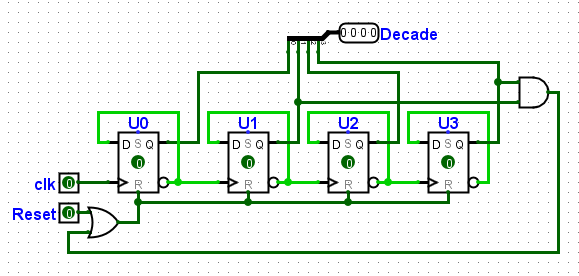
\includegraphics[width=\maxwidth{.95\linewidth}]{gfx/06-03}
	\caption{Asynchronous Decade Counter}
	\label{fig:06-03}
\end{figure}

The following list describes the operation of the counter in Figure \ref{fig:06-03}:

\begin{description}
	\item [Reset is activated] All flip-flops are reset so \textit{Q} is low and \textit{Q'} is high.
	
	%%%%%%%%%%%%%%%
	\item [Tick 1] \textit{U0} clocked: \textit{Q0} \textuparrow \: \textemdash \: \textit{Q'0} \textdownarrow
	
	%%%%%%%%%%%%%%%
	\item [Tick 2] \textit{U0} clocked: \textit{Q0} \textdownarrow \: \textemdash \: \textit{Q'0} \textuparrow
	
	\hspace{14pt}\textit{U1} clocked: \textit{Q1} \textuparrow \: \textemdash \: \textit{Q'1} \textdownarrow
	
	%%%%%%%%%%%%%%%
	\item [Tick 3] \textit{U0} clocked: \textit{Q0} \textuparrow \: \textemdash \: \textit{Q'0} \textdownarrow
	
	%%%%%%%%%%%%%%%
	\item [Tick 4] \textit{U0} clocked: \textit{Q0} \textdownarrow \: \textemdash \: \textit{Q'0} \textuparrow
	
	\hspace{14pt}\textit{U1} clocked: \textit{Q1} \textdownarrow \: \textemdash \: \textit{Q'1} \textuparrow
	
	\hspace{14pt}\textit{U2} clocked: \textit{Q2} \textuparrow \: \textemdash \: \textit{Q'2} \textdownarrow
	
	%%%%%%%%%%%%%%%
	\item [Tick 5] \textit{U0} clocked: \textit{Q0} \textuparrow \: \textemdash \: \textit{Q'0} \textdownarrow
	
	%%%%%%%%%%%%%%%
	\item [Tick 6] \textit{U0} clocked: \textit{Q0} \textdownarrow \: \textemdash \: \textit{Q'0} \textuparrow
	
	\hspace{14pt}\textit{U1} clocked: \textit{Q1} \textuparrow \: \textemdash \: \textit{Q'1} \textdownarrow
	
	%%%%%%%%%%%%%%%
	\item [Tick 7] \textit{U0} clocked: \textit{Q0} \textuparrow \: \textemdash \: \textit{Q'0} \textdownarrow
	
	%%%%%%%%%%%%%%%
	\item [Tick 8] \textit{U0} clocked: \textit{Q0} \textdownarrow \: \textemdash \: \textit{Q'0} \textuparrow
	
	\hspace{14pt}\textit{U1} clocked: \textit{Q1} \textdownarrow \: \textemdash \: \textit{Q'1} \textuparrow
	
	\hspace{14pt}\textit{U2} clocked: \textit{Q2} \textdownarrow \: \textemdash \: \textit{Q'2} \textuparrow
	
	\hspace{14pt}\textit{U3} clocked: \textit{Q3} \textuparrow \: \textemdash \: \textit{Q'3} \textdownarrow

	%%%%%%%%%%%%%%%
	\item [Tick 9] \textit{U0} clocked: \textit{Q0} \textuparrow \: \textemdash \: \textit{Q'0} \textdownarrow

	%%%%%%%%%%%%%%%
	\item [Tick 10] \textit{U1} clocked: \textit{Q0} \textuparrow \: \textemdash \: \textit{Q'0} \textdownarrow
	
	\noindent Both inputs for the \texttt{AND} gate are momentarily high and that sends a reset signal that causes all outputs to go low.
	
\end{description}

As the clock continues the counter would cycle through the binary values 0000 - 1001. The following table lists the \textit{Decade} counter output as indicated by the \textit{Q} values at each tick listed above.

\begin{table}[H]
	\sffamily
	\newcommand{\head}[1]{\textcolor{white}{\textbf{#1}}}		
	\begin{center}
		\rowcolors{2}{gray!10}{white} % Color every other line a light gray
		\begin{tabular}{cc} 
			\rowcolor{black!75}
			\head{Tick} & \head{Output} \\
			Reset & 0000 \\
			1 & 0001 \\
			2 & 0010 \\
			3 & 0011 \\
			4 & 0100 \\
			5 & 0101 \\
			6 & 0110 \\
			7 & 0111 \\
			8 & 1000 \\
			9 & 1001 \\
		 10 & 0000
		\end{tabular}
	\end{center}
	\caption{Decade Counter Output}
	\label{tab0603}
\end{table}

\subsection{Synchronous Ring Counter}

In a ring counter the high bit is shifted through all of the bits one at a time. This counter is very useful in controlling subcircuits since the high bit in the counter can activate the next subcircuit in the sequence.

The ring counter presented here is also a synchronous circuit; that is, each clock pulse is applied to all of the flip-flops instead of just the first stage. The \textit{Q} output from each flip-flop is used but \textit{Q'} is not needed at all. Also, there is a feedback line from \textit{U3} to the data input port of \textit{U0} so when the \textit{Q} output of \textit{U3} goes high that is made available to \textit{U0} and loop that value back through the circuit.

\begin{figure}[H]
	\centering
	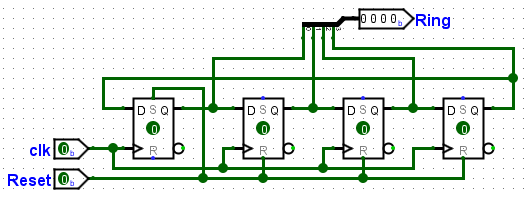
\includegraphics[width=\maxwidth{.95\linewidth}]{gfx/06-04}
	\caption{Synchronous Ring Counter}
	\label{fig:06-04}
\end{figure}

The following list describes the operation of the counter in Figure \ref{fig:06-04}. Students should open the counter circuit with \LE then use the ``poke'' tool to set the clock high then low (one complete clock cycle) as they follow the description below.

\begin{description}
	\item [Reset is activated] \textit{U0} is set and \textit{U1}-\textit{U3} are reset so the counter is seeded with a single high bit to shift.
	
	%%%%%%%%%%%%%%%
	\item [Tick 1] \textit{Q0} \textdownarrow \: \textemdash \: \textit{Q1} \textuparrow
	
	%%%%%%%%%%%%%%%
	\item [Tick 2] \textit{Q1} \textdownarrow \: \textemdash \: \textit{Q2} \textuparrow
	
	%%%%%%%%%%%%%%%
	\item [Tick 3] \textit{Q2} \textdownarrow \: \textemdash \: \textit{Q3} \textuparrow
	
	%%%%%%%%%%%%%%%
	\item [Tick 4] \textit{Q3} \textdownarrow \: \textemdash \: \textit{Q1} \textuparrow
	
\end{description}

As the clock continues the counter would cycle through the binary values 0001 - 1000. The following table lists the \textit{ring} counter output as indicated by the \textit{Q} values at each tick listed above.

\begin{table}[H]
	\sffamily
	\newcommand{\head}[1]{\textcolor{white}{\textbf{#1}}}		
	\begin{center}
		\rowcolors{2}{gray!10}{white} % Color every other line a light gray
		\begin{tabular}{cc} 
			\rowcolor{black!75}
			\head{Tick} & \head{Output} \\
			Reset & 0001 \\
			1 & 0010 \\
			2 & 0100 \\
			3 & 1000 \\
			4 & 0001 \\
			5 & 0010 \\
			6 & 0100 \\
			7 & 1000 \\
			8 & 0001 
		\end{tabular}
	\end{center}
	\caption{Ring Counter Output}
	\label{tab0604}
\end{table}

\subsection{Synchronous Johnson Counter}

A Johnson Counter is similar to a ring counter in that a high bit value is shifted through the entire binary word. The difference is that the feedback loop comes from the \textit{Q'} output of the last stage rather than the \textit{Q} output. This type of counter is sometimes called a ``twisted tail'' counter since the \textit{Q'} output is fedback.

\begin{figure}[H]
	\centering
	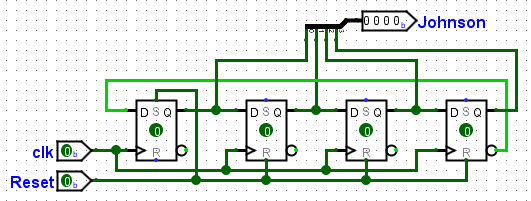
\includegraphics[width=\maxwidth{.95\linewidth}]{gfx/06-05}
	\caption{Synchronous Johnson Counter}
	\label{fig:06-05}
\end{figure}

The following list describes the operation of the counter in Figure \ref{fig:06-05}. Students should open the counter circuit with \LE then use the ``poke'' tool to set the clock high then low (one complete clock cycle) as they follow the description below.

\begin{description}
	\item [Reset is activated] \textit{U0} is set and \textit{U1}-\textit{U3} are reset so the counter is seeded with a single high bit to shift.
	
	%%%%%%%%%%%%%%%
	\item [Tick 1] \textit{Q1} \textuparrow 
	
	%%%%%%%%%%%%%%%
	\item [Tick 2] \textit{Q2} \textuparrow
	
	%%%%%%%%%%%%%%%
	\item [Tick 3] \textit{Q3} \textuparrow 
	
	%%%%%%%%%%%%%%%
	\item [Tick 4] \textit{Q0} \textdownarrow

	%%%%%%%%%%%%%%%
	\item [Tick 5] \textit{Q1} \textdownarrow

	%%%%%%%%%%%%%%%
	\item [Tick 6] \textit{Q2} \textdownarrow
	
	%%%%%%%%%%%%%%%
	\item [Tick 7] \textit{Q3} \textdownarrow

	%%%%%%%%%%%%%%%
	\item [Tick 8] \textit{Q0} \textuparrow

\end{description}

As the clock continues the counter would cycle through the binary values 0000 - 1111. The following table lists the \textit{Johnson} counter output as indicated by the \textit{Q} values at each tick listed above.

\begin{table}[H]
	\sffamily
	\newcommand{\head}[1]{\textcolor{white}{\textbf{#1}}}		
	\begin{center}
		\rowcolors{2}{gray!10}{white} % Color every other line a light gray
		\begin{tabular}{cc} 
			\rowcolor{black!75}
			\head{Tick} & \head{Output} \\
			Reset & 0001 \\
			1 & 0011 \\
			2 & 0111 \\
			3 & 1111 \\
			4 & 1110 \\
			5 & 1100 \\
			6 & 1000 \\
			7 & 0000 \\
			8 & 0001 
		\end{tabular}
	\end{center}
	\caption{Johnson Counter Output}
	\label{tab0605}
\end{table}

\subsection{Main}

The \lstinline[columns=fixed]|main| circuit provides a human interface to try out each of the counters by dropping them in place of the \textit{Up} counter.

\begin{figure}[H]
	\centering
	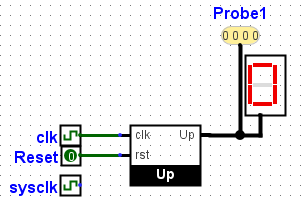
\includegraphics[width=\maxwidth{.95\linewidth}]{gfx/06-06}
	\caption{Main Circuit}
	\label{fig:06-06}
\end{figure}

Notice that there are two clocks in the \lstinline[columns=fixed]|main| circuit. \textit{Clk} is linked to the counter being tested and is used within the counter circuit to advance the count. \textit{Sysclk} is used by the \LE chronogram as described in the next section of this document.

\subsection{Chronogram}

\LE can generate a timing diagram, called a \textit{chronogram}, for a sequential circuit. That is a representation of the various signals in a circuit and how those signals change over time. Figure \ref{fig:06-07} is the timing diagram for an Up counter.

\begin{figure}[H]
	\centering
	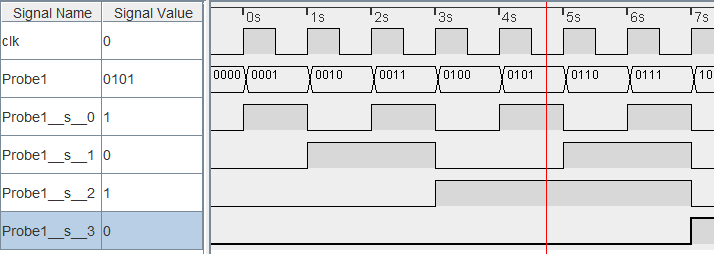
\includegraphics[width=\maxwidth{.95\linewidth}]{gfx/06-07}
	\caption{Timing Diagram for Up Counter}
	\label{fig:06-07}
\end{figure}

At the top of Figure \ref{fig:06-07} is a scale that indicates the number of seconds that the counter has been operating. The first trace is the input clk signal. The clock goes high at the start of each second and then goes low at the half-second mark. Under the clock is the ``Probe1'' signal. Because that is a four-bit number \LE displays the number, but under that number is a breakout of the four bits that make up that number. Thus, at time zero ``Probe1'' is 0001 and ``Probe1\_s\_0'' (that stands for ``Probe 1, Signal 0'') is high while the other bits are low. The \LE \textit{chronogram} includes a cursor indicated by a red line (found just before the five second tick in Figure \ref{fig:06-07}) that can be placed anywhere along the diagram. The cursor sets the values of each signal in the area on the left edge of the diagram, so the cursor in Figure \ref{fig:06-07} is pointing to a spot where the \textit{clk} is low, \textit{Probe1} is at 0101, and so forth.

Follow the next steps to use the chronogram. Notes: the chronogram will only check subcircuits that are found on the  \lstinline[columns=fixed]|main| subcircuit. Therefore, in order to create a timing diagram all subcircuits need to be combined on \lstinline[columns=fixed]|main|. The labs completed in this manual have been designed to use the \lstinline[columns=fixed]|main| subcircuit as the human interface so the chronogram feature will work well with these circuits. 

\begin{enumerate}
	\item In the \lstinline[columns=fixed]|main| subcircuit, add a ``sampling clock'' labeled \textit{sysclk} (this name is important, do not change it to something else). The sampling clock is only used by the \textit{chronogram} and will not show up in the timing diagram. It should not be connected to any other components and can be placed anywhere on \lstinline[columns=fixed]|main|. Set the properties for \textit{sysclk} to a 1 Tick high duration and a 1 Tick low duration (this is the default). 
	\item Add a circuit master clock labeled \textit{clk}. This is the clock that will be used to trigger all components in the circuit. Set the properties for \textit{clk} to a 4 Tick high duration and a 4 Tick low duration.
	\item Set \textsc{Simulate -> Tick Frequency} to 4 Hertz. This will simulate a clock that ticks once per second, as in Figure \ref{fig:06-07}. While the actual tick frequency can be changed later to ``speed up'' the circuit, a one-second tick is useful for learning how the \textit{chronogram} works.
	\item Click \textsc{Simulate -> Chronogram} to set up the \textit{chronogram}. Figure \ref{fig:06-08} illustrates the initial setup screen for the \textit{chronogram}.

	\begin{figure}[H]
		\centering
		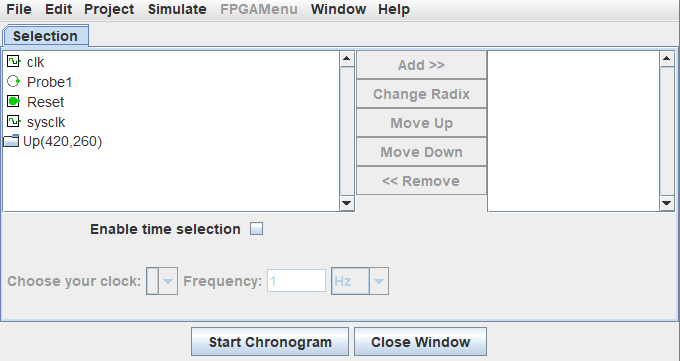
\includegraphics[width=\maxwidth{.95\linewidth}]{gfx/06-08}
		\caption{Set Up Chronogram}
		\label{fig:06-08}
	\end{figure}

	\item Click \textit{sysclk} in the left panel and then click \textit{Add >>} to add that signal to the \textit{chronogram}. The ``-2'' following the \textit{sysclk} name in the right panel indicates that it is a binary signal.\marginpar{NOTE: \textit{sysclk} must be added to the \textit{chronogram} or it will not sample the circuit; however, the \textit{sysclk} signal will not actually show up in the timing diagram.} It is probably best to add the \textit{sysclk} signal first so it is not overlooked.
	\item Click \textit{clk} in the left panel and then click \textit{Add >>} to add that signal to the \textit{chronogram}.
	\item Click \textit{Probe1} in the left panel and then click \textit{Add >>} to add that signal to the \textit{chronogram}.
	\item Click ``Enable time selection'' and chose \textit{clk} as the clock with a frequency of 1 Hertz.
	\item The \textit{chronogram} setup should look like Figure \ref{fig:06-09}.
	
	\begin{figure}[H]
		\centering
		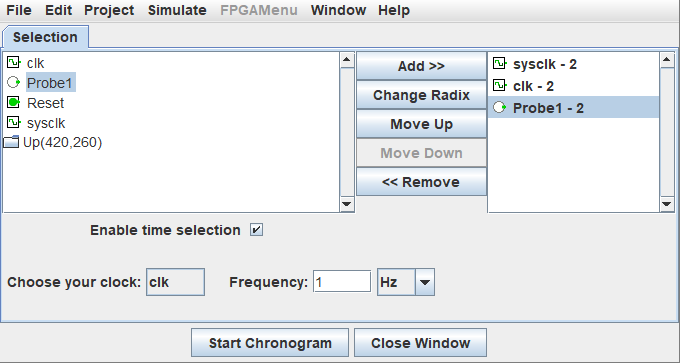
\includegraphics[width=\maxwidth{.95\linewidth}]{gfx/06-09}
		\caption{Chronogram Ready}
		\label{fig:06-09}
	\end{figure}

	\item Click \textit{Start Chronogram} and the screen illustrated in Figure \ref{fig:06-10} pops up.
	
	\begin{figure}[H]
		\centering
		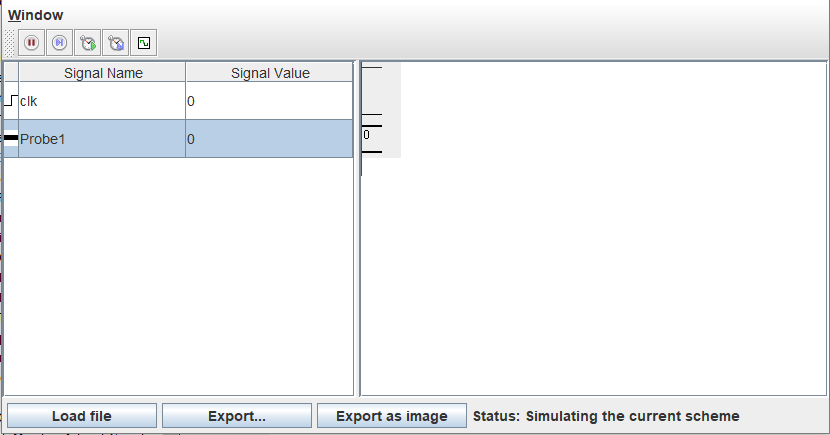
\includegraphics[width=\maxwidth{.95\linewidth}]{gfx/06-10}
		\caption{Chronogram Starting}
		\label{fig:06-10}
	\end{figure}
	
	\item Right-click on the \textit{Probe1} signal and set the format for binary. The format can be set for any radix but to match this lab binary numbers should be specified.
	\item Right-click on the \textit{Probe1} signal and enable \textit{Expand} to see all four signals that create \textit{Probe1}.
	\item At this point, the chronogram should look like Figure \ref{fig:06-11}.
	
	\begin{figure}[H]
		\centering
		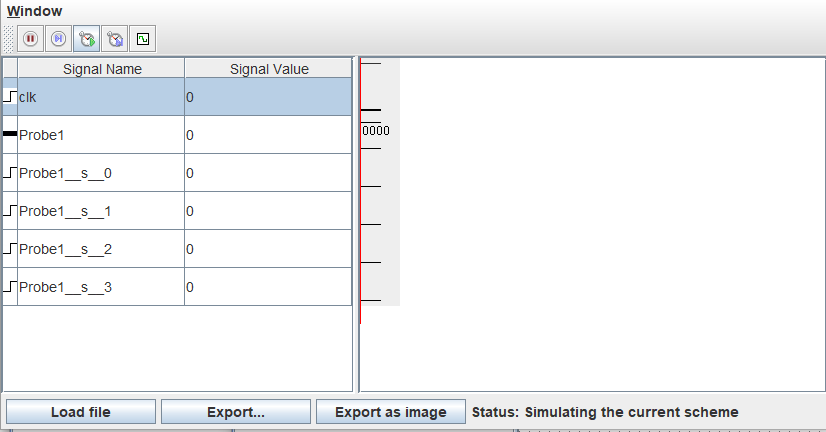
\includegraphics[width=\maxwidth{.95\linewidth}]{gfx/06-11}
		\caption{Chronogram At Zero Time}
		\label{fig:06-11}
	\end{figure}
	
	\item The \textit{chronogram} has five buttons that control the simulator.
	
	\begin{figure}[H]
		\centering
		
\includegraphics[width=\maxwidth{.95\linewidth}]{gfx/06-12}
		\caption{Chronogram Controls}
		\label{fig:06-12}
	\end{figure}
	
	\begin{itemize}
		\item Button One: Start/Stop the simulation.
		\item Button Two: Simulate one step.
		\item Button Three: Start/Stop \textit{sysclk}. This will ``turn on'' the chronogram and begin creating a timing diagram.
		\item Button Four: Step one \textit{sysclk} tick. This will tick the \textit{sysclk} one time. Since this lab set up the \textit{sysclk} for four ticks per second this button would need to be clicked four times to extend the timing diagram one second.
		\item Button Five: Step one \textit{clk} tick. This extends the timing diagram by one complete clock tick, or one second in this circuit.
	\end{itemize}
	
	\item Click button three to start the \textit{chronogram} and watch the timing diagram unfold. After a few seconds click that button a second time to stop the \textit{chronogram}.
	
	\item The following can be done once the timing diagram is complete.
	
	\begin{itemize}
		\item Click on the timing diagram to set the cursor (indicated by a red line). Once the cursor is set the values for each signal at the cursor's location are printed next to the signal's label on the left edge of the timing diagram.
		\item Hover the mouse over the timing diagram and roll the mouse wheel to zoom the timing diagram appearance.
		\item Click ``Export'' to save the timing diagram signal levels in a text file. That file can later be loaded to reevaluate the timing diagram.
		\item Click ``Export as image'' to save the timing diagram as a PNG file.
	\end{itemize}
	
\end{enumerate}

\section{Challenge}

This lab includes several different timers. Place all of them on a single subcircuit named \lstinline[columns=fixed]|Universal| that includes an output mux so a user can select the type of counter output desired. Place the \lstinline[columns=fixed]|Universal| circuit on \lstinline[columns=fixed]|main| and wire appropriate inputs and outputs.

Set up the chronogram for the ring counter and create a ten-second timing diagram for that counter. Save the timing diagram as a PNG image named ``RingCounter.''

\section{Deliverable}

To receive a grade for this lab, complete the Challenge. Be sure the standard identifying information is at the top left of the \lstinline{main} circuit: 

\bigskip
% The minipage environment keeps the three lines together - no page break.
\begin{minipage}{\linewidth}
	\begin{verbatim}
	George Self
	Lab 06: Counters
	March 17, 2018
	\end{verbatim}
\end{minipage}
\bigskip

Save the circuit with this name: \textit{Lab07\_counter} and submit that along with \textit{RingCounter.PNG} for grading.

  
%*******************************************
% Lab 08: ALU
%*******************************************
\chapter{Arithmetic Logic Unit (ALU)}\label{alu}

\section{Purpose}

In this lab you will build an \acf{ALU}. An \ac{ALU} is an important digital logic device used to perform all sorts of arithmetic and logic functions in a circuit. The commercial 74181 \ac{ALU} has two four-bit data inputs along with a one-bit mode (M) and a four-bit select input. Depending on those settings, the device will complete one of the functions listed in Table \ref{tab0301}.

\begin{table}[H]
	\sffamily
	\newcommand{\head}[1]{\textcolor{white}{\textbf{#1}}}		
	\begin{center}
		\rowcolors{2}{gray!10}{white} % Color every other line a light gray
		\begin{tabular}{ccc} 
			\rowcolor{black!75}
			\head{Select} & \head{Logic (M=1)} &\head{Arithmetic (M=0)} \\
			0000 & A' & A \\
			0001 & (A + B)' & A + B \\
			0010 & A'B & A + B' \\
			0011 & Logical 0 & minus 1 (2's Comp) \\
			0100 & (AB)' & A + AB' \\
			0101 & B' & (A + B) plus AB' \\
			0110 & A XOR B & A minus B minus 1 \\
			0111 & AB' & AB' minus 1 \\
			1000 & A' + B & A plus AB \\
			1001 & (A XOR B)' & A plus B \\
			1010 & B & (A + B') plus AB \\
			1011 & AB & AB minus 1 \\
			1100 & Logical 1 & A plus A \\
			1101 & A + B' & (A + B) plus A \\
			1110 & A + B & (A + B') plus A \\
			1111 & A & A minus 1
		\end{tabular}
	\end{center}
	\caption{Function Table for 74181 ALU}
	\label{tab0301}
\end{table}

Notes: in the ``Arithmetic'' column, the + sign indicates logic \textit{OR} while the words \textit{plus} and \textit{minus} indicate arithmetic add and subtract operations. The value of \textit{A plus A} is the same as shifting the bits left to the next most significant position.

The \ac{ALU} built in this lab is not as complex as an 74181 \ac{IC}, however it demonstrates the basic functions of an \ac{ALU}.

\section{Procedure}

Load the \ac{ALU} starter circuit in \textit{Logisim-evolution}. 

\subsection{main}

The \lstinline[columns=fixed]|main| circuit does nothing more than provide a human-friendly interface for the rest of the \ac{ALU}. That interface include two eight-bit inputs (labeled \textit{A} and \textit{B}), a three-bit select, a one-bit mode, a carry-in and carry-out bit (so the \ac{ALU} could be chained to another), a \textit{compare} output (TRUE if the two inputs are equal), and a eight-bit output (labeled \textit{ALU\_Out}). In operation, numbers are entered at \textit{A} and \textit{B}, the mode and select are set, and then the result is read on \textit{ALU\_Out}.

\begin{figure}[H]
	\centering
	\includegraphics[width=\maxwidth{.95\linewidth}]{gfx/alu-01}
	\caption{ALU main}
	\label{fig:alu-01}
\end{figure}

\subsection{ALU}

The \lstinline[columns=fixed]|ALU| subcircuit is designed to contain the logic that routes \textit{A}, \textit{B}, and \textit{Sel} to two other subcircuits, \lstinline[columns=fixed]|arith\_main| or \lstinline[columns=fixed]|logic\_main|. It then uses a multiplexer to route the output of one of those subcircuits to an output port depending on the setting of the \textit{Mode} bit. Note that the inputs are sent to both subcircuits but only the output specified by the \textit{Mode} is returned to the user. This type of logic is also used in Labs \ref{arith} and \ref{logic}.

The Arithmetic and Logic subcircuits that were built in Labs \ref{arith} and \ref{logic} will be reused for this lab. This is the way that circuit designers can reuse their work to build more complex circuits without having to reinvent the proverbial wheel for every project. To reload those old labs, click \textsc{Project -> Load Library -> Logisim-evolution Library}\footnote{In order to load labs for reuse it is important to store the project files in the same folder.}. Find Lab \ref{arith}, Arithmetic, and click \textit{Open}. That lab is now available as a library in the library list on the left side of the \LE workspace. Follow the same procedure to also load Lab \ref{logic}, Logic, as a library. 

Open the Arithmetic library and drop the \lstinline[columns=fixed]|arithmetic| subcircuit in the \lstinline[columns=fixed]|ALU| subcircuit. This process is exactly like dropping a device from the Wiring library and should not be difficult to figure out. In the same way, drop the \lstinline[columns=fixed]|logic| subcircuit from the Logic library onto the \lstinline[columns=fixed]|ALU| subcircuit.

At this point, the ALU subcircuit should resemble Figure \ref{fig:alu-02}.

\begin{figure}[H]
	\centering
	\includegraphics[width=\maxwidth{.95\linewidth}]{gfx/alu-02}
	\caption{ALU Subcircuit}
	\label{fig:alu-02}
\end{figure}

\subsection{Challenge}

Continue to wire the \lstinline[columns=fixed]|ALU| subcircuit. Note: the inputs and outputs that were provided will need to be repositioned in order to complete this build.

\begin{itemize}
	\item Wire the \textit{CI} input to the \textit{CI} port on the \textit{arithmetic} device
	\item Wire inputs A and \item  to ports \textit{A} and \textit{B} on both devices.
	\item Wire the \textit{Sel} input to the \textit{Sel} ports on both devices.
	\item The \textit{arithmetic} \textit{CO} and \textit{Cmp} ports should be wired to the \textit{CO} and \textit{Cmp} outputs
	\item Add an 8-bit, 2-input multiplexer. The inputs should be wired to the output ports on both devices. The multiplexer select bit should be wired to the \textit{Mode} input. Finally, the multiplexer output should be wired to the \textit{ALU\_Out} output.
\end{itemize}


\subsection{Testing the Circuit}

The \ac{ALU} can be tested from the \lstinline[columns=fixed]|main| circuit. Several values can be entered on \textit{A} and \textit{B} and then various arithmetic and logic operations selected. The outputs for each check should be accurate. A test vector file has been provided for this lab so all of the ALU's functions can be exercised.

\section{Deliverable}

To receive a grade for this lab, complete the Challenge. Be sure the standard identifying information is at the top left of the \textit{main} circuit, similar to this: 

\bigskip
% The minipage environment keeps the three lines together - no page break.
\begin{minipage}{\linewidth}
	\begin{verbatim}
	George Self
	Lab 08: ALU
	February 18, 2018
	\end{verbatim}
\end{minipage}
\bigskip

Save the file with this name: \emph{\texttt{Lab08\_ALU}} and submit that file for grading.
 
%%*******************************************
% Lab 03: Priority Encoder
%*******************************************
\chapter{Priority Encoder}

\section{Purpose}

Often a circuit will receive data from several sources at one time and there must be a way to prioritize those inputs. This circuit creates a simple priority encoder for nine different inputs. This is a fairly simple circuit but is best explained by building and ``playing around'' with it rather than attempting to understand a printed text; thus, the explanation for this lab is somewhat limited.

\section{Procedure}

Start \LE and create a subcircuit named \lstinline[columns=fixed]|Encoder|. Open that subcircuit and place 12 \texttt{AND} gates as illustrated in Figure \ref{fig:03-01}.

\begin{figure}[H]
	\centering
	\includegraphics[width=\maxwidth{.95\linewidth}]{gfx/03-01}
	\caption{AND Gates}
	\label{fig:03-01}
\end{figure}

The gates have one data bit and these properties:

\begin{itemize}
	\item \textbf{U1}: Five inputs, numbers two, three, and four negated.
	\item \textbf{U2}: Four inputs, numbers two and three negated.
	\item \textbf{U3}: Three inputs, number two negated.
	\item \textbf{U4}: Two inputs, none negated.
	\item \textbf{U5}: Four inputs, numbers two and three negated.
	\item \textbf{U6}: Four inputs, numbers one and two negated.
	\item \textbf{U7-U12}: Two inputs, none negated. 
\end{itemize}

Many of the output signals need to be combined with \texttt{OR} gates and those should be added next, as in Figure \ref{fig:03-02}. Note: U16 is a \texttt{NOR} (\textit{Gates} library) gate.

\begin{figure}[H]
	\centering
	\includegraphics[width=\maxwidth{.95\linewidth}]{gfx/03-02}
	\caption{OR Gates Added}
	\label{fig:03-02}
\end{figure}

This encoder is designed to prioritize nine input lines so nine inputs must be added, as illustrated in Figure \ref{fig:03-03}.

\begin{figure}[H]
	\centering
	\includegraphics[width=\maxwidth{.95\linewidth}]{gfx/03-03}
	\caption{Inputs Added}
	\label{fig:03-03}
\end{figure}

Wiring this circuit is the most challenging part of the build. As illustrated in Figure \ref{fig:03-04}, the inputs are wired to several different \texttt{AND} gates.

\begin{figure}[H]
	\centering
	\includegraphics[width=\maxwidth{.95\linewidth}]{gfx/03-04}
	\caption{Wiring the Encoder}
	\label{fig:03-04}
\end{figure}

Finally, four output ports are added, as illustrated in Figure \ref{fig:03-05}. 

\begin{figure}[H]
	\centering
	\includegraphics[width=\maxwidth{.95\linewidth}]{gfx/03-05}
	\caption{Nine-line Priority Encoder}
	\label{fig:03-05}
\end{figure}

This circuit is designed to output a \acf{BCD} number, so no further conversion is needed to be able to read the highest priority input line. At this point, the circuit is complete and the \textit{poke} tool can be used to change the inputs and observe how that high input bit drives the outputs.

To finish the project, open the \lstinline[columns=fixed]|main| circuit and drop the \lstinline[columns=fixed]|Encoder| on the drawing canvas. Add nine inputs and label them \textit{In1} through \textit{In9}. Place a four-bit output labeled \textit{PriOut} and wire the four outputs through a splitter to that output port. To make it easier to read the \ac{BCD} number, connect a Hex Digit Display (\textit{Input/Output} library) to the four-bit bus between the splitter and output port. The completed \lstinline[columns=fixed]|main| circuit is illustrated in Figure \ref{fig:03-06}.

\begin{figure}[H]
	\centering
	\includegraphics[width=\maxwidth{.95\linewidth}]{gfx/03-06}
	\caption{Main Circuit}
	\label{fig:03-06}
\end{figure}

In Figure \ref{fig:03-06}, notice that two inputs are selected, \textit{In4} and \textit{In6}. Since \textit{In6} is a higher priority (it is a larger number), the output is set for six and \textit{In4} is ignored.

\subsection{Testing the Circuit}

The circuit is now complete. It should be tested by entering various combinations of inputs and observing that the output always displays the highest numbered input. 

\section{Deliverable}

To receive a grade for this lab, create the Nine-line Priority Encoder circuit as defined in this lab. Be sure the standard identifying information is at the top left of the circuit, similar to this:

\bigskip
% The minipage environment keeps the three lines together - no page break.
\begin{minipage}{\linewidth}
	\begin{verbatim}
	George Self
	Lab 03: Nine-line Priority Encoder
	February 18, 2018
	\end{verbatim}
\end{minipage}
\bigskip

Save the file with this name: \emph{\texttt{Lab03\_Encoder}} and submit that file for grading. 
%%****************************************
% Lab 07: Timer
%****************************************
\chapter{Timer}

\section{Purpose}

A timer is used to time events. This lab creates a timer where the minimum and maximum counts can be set and counts both up and down. The timer assumes an input clock pulse at 1 Hz (or 60 pulses per minute) but for testing, the clock can be set to any value.

\section{Procedure}

The lab starter circuit includes several versions of the timer as an illustration of the thought process used to develop the final product.

\begin{itemize}
	\item \textbf{Timer\_V1}. This is little more than a test of the Counter (\textit{Memory} library) component. The various inputs were wired so both the \textit{Load} and \textit{Up} input pins could be tested. Instead of a clock pulse, a Button (\textit{Input/Output} library) was used for better control over the device. A Bin2BCD (\textit{BFH mega functions} library) device was used for easier interpretation of the output.
	\item \textbf{Timer\_V2}. The first circuit was expanded such that both the minimum and maximum counts could be specified. Note that the multiplexer (\textit{Plexers} library) selects whether the minimum or maximum number is loaded depending on whether the count is Up or Down.
	\item \textbf{Timer\_V3}. This is the version of the timer that will be completed for this lab.
\end{itemize}

\subsection{Timer\_V3}

Complete the circuit to match Figure \ref{fig:07-01}.

\begin{figure}[H]
	\centering
	\includegraphics[width=\maxwidth{.95\linewidth}]{gfx/07-01}
	\caption{Completed Timer}
	\label{fig:07-01}
\end{figure}

In the timer circuit, the key is the comparator in the lower left corner. That device compares the binary output of the counter to either the minimum or maximum requested value and if they are equal the comparator sends a reset signal to start the count over. 

There are two multiplexers with a subtle, but important, difference. The Maximum input value is wired to the top input of the top multiplexer but the bottom input of the bottom multiplexer. The result is the when the count is ``Up'' the Minimum input is loaded into the counter but the Maximum input is used in the compare, so the counter starts at the minimum and counts up to the maximum. The opposite is true for a ``Down'' count.

Finally, the BCD output is combined by a splitter (\textit{Wiring} library) into a 12-bit bus for transmission.

\subsection{Testing the Circuit}

The \lstinline[columns=fixed]|Timer_V3| subcircuit should be added to the \lstinline[columns=fixed]|main| circuit and wired as in Figure \ref{fig:07-02}.

\begin{figure}[H]
	\centering
	\includegraphics[width=\maxwidth{.95\linewidth}]{gfx/07-02}
	\caption{Timer Main Circuit}
	\label{fig:07-02}
\end{figure}
 
To test the circuit:

\begin{enumerate}
	\item Enter binary four for a minimum value and eight for a maximum value. (Actually, any values can be entered but four and eight are enough to test the circuit.) 
	\item Poke \textit{Up\_Down} to change its value to one so the circuit counts up.
	\item Poke the Reset button and observe that the BCD out changes to 004.
	\item Activate the clock \textsc{Simulate -> Ticks Enabled} and observe that it counts up from four to eight and then resets to four. If the speed of the timer is not reasonable then the \textsc{Simulate -> Tick Frequency} can be adjusted.
	\item Poke \textit{Up\_Down} to change the count to down and observe that the timer now counts from eight to four and resets.
\end{enumerate}

\section{Challenge}

As designed, the output of this circuit is an integer count. If it were set for counting seconds then the count of seconds would increase from 59 to 60 then 61 rather than going 0:59, 1:00, 1:01 as expected. Rewrite the \lstinline[columns=fixed]|Timer_V3| subcircuit so the output is two BCD numbers: minutes and seconds. As a hint, the Divider (\textit{Arithmetic} library) device products an integer (``modulus'') division along with a remainder. It should help to divide the count by 60, use the whole number as ``minutes'' and the remainder as the ``seconds.''

\section{Deliverable}

To receive a grade for this lab, complete the Challenge. Be sure the standard identifying information is at the top left of the \lstinline{main} circuit, similar to: 

\bigskip
% The minipage environment keeps the three lines together - no page break.
\begin{minipage}{\linewidth}
	\begin{verbatim}
	George Self
	Lab 07: Timer
	March 1, 2018
	\end{verbatim}
\end{minipage}
\bigskip

Save the file with this name: \emph{\texttt{Lab07\_Timer}} and submit that file for grading.

 
%%**************************************************************
% Lab 09: ROM
%**************************************************************
\chapter{ROM}\label{Lab09}

\section{Purpose}

\begin{wrapfigure}{O}{0.2\textwidth}
	\caption*{} % No text, wraps badly in very narrow space (does print fig number)
	% to not print a fig number use \caption*{}
	\label{fig:09-01} 
	\centering
	\includegraphics[width=0.2\textwidth]{gfx/09-01} 
\end{wrapfigure}
This lab introduces students to \acf{ROM} and builds a fun application: The \textit{Magic 8-Ball}. This was a toy that was developed in the 1950s and was popular throughout the 1960s. It was a small plastic sphere with the markings of an 8-ball. If the user ``asked it a question'' and then turned the toy upside down the answer would magically appear in a small window on the bottom of the ball.

\section{Procedure}

Start a new \LE project and create a subcircuit named \lstinline[columns=fixed]|Magic_8_Ball|. Open that circuit and place a ROM (\textit{Memory} library) device near the center of the drawing canvas. Set the ROM properties for an \textit{Address Bit Width} of 12 and a \textit{Data Bit Width} of 8\footnote{The provided starter circuit already contains the \lstinline[columns=fixed]|Magic_8_Ball| subcircuit along with two devices needed in the early part of the build.}.

\begin{figure}[H]
	\centering
	\includegraphics[width=\maxwidth{.95\linewidth}]{gfx/09-02}
	\caption{Placing ROM}
	\label{fig:09-02}
\end{figure}

A ROM stores data that is accessed by setting an address on the inputs at the top left of the device and then reading the contents of that address on the 8-bit bus on the right side of the device. By attaching a counter to the ROM address port several consecutive addresses can be ``stepped through'' to output a message. Attach a Counter (\textit{Memory} library) with 12 Data Bits to the address port of the ROM, as in Figure \ref{fig:09-03}.

\begin{figure}[H]
	\centering
	\includegraphics[width=\maxwidth{.95\linewidth}]{gfx/09-03}
	\caption{ROM With Counter}
	\label{fig:09-03}
\end{figure}

According to Wikipedia\footnote{\url{https://en.wikipedia.org/wiki/Magic_8-Ball}}, the Magic 8-Ball featured 20 sayings: 

\begin{verbatim}
 1 001 It is certain
 2 00f It is decidedly so
 3 022 Without a doubt
 4 032 Yes definitely
 5 041 You may rely on it
 6 054 As I see it yes
 7 064 Most likely
 8 070 Outlook good
 9 07d Yes
10 081 Signs point to yes
11 094 Reply hazy try again
12 0a9 Ask again later
13 0b8 Better not tell you now
14 0d1 Cannot predict now
15 0e4 Concentrate and ask again
16 0fe Do not count on it
17 111 My reply is no
18 120 My sources say no
19 132 Outlook not so good
20 146 Very doubtful
\end{verbatim}

The \textit{Magic 8-Ball} simulator built in this lab uses those same 20 saying. In the above chart, each saying is numbered and the start point in ROM (using hexadecimal notation) for each saying is also noted. Thus, saying one starts on ROM byte 001, saying two starts on ROM byte 00f, saying three starts on ROM byte 022, and so forth.

The content of the ROM device must be loaded before it can be used and that content is provided in \emph{\texttt{Lab09\_ROM.txt}} accompanying this lab. To load the ROM device, click it one time and then click the ``(click to edit)'' link in its properties panel. In the ROM editor window that pops up, click the ``open'' button and navigate to the ROM memory file. Click ``close window'' to load the ROM device and make it ready for service\footnote{The ROM device provided with the starter circuit is pre-loaded so it will not be necessary to load it again. However, this information is left here for students who may want to load the ROM for practice.}.

The start point for each saying, as indicated on the above table, is stored in a Constant (\textit{Wiring} library) then a Mux (\textit{Plexers} library) with five select bits is used to transmit a message start location to the counter so it can be read from the ROM device. Figure \ref{fig:09-04} illustrates the circuit at this point\footnote{The multiplexer provided with the starter circuit already has the various constants attached. Students who wish to do so can create their own multiplexer by using the start addresses in the ``Sayings'' listing above.}.

\begin{figure}[H]
	\centering
	\includegraphics[width=\maxwidth{.95\linewidth}]{gfx/09-04}
	\caption{ROM Filter Mux}
	\label{fig:09-04}
\end{figure}

A five-bit Random Generator (\textit{Memory} library) is used to select a random message. Figure \ref{fig:09-05} illustrates the placement of the random generator.

\begin{figure}[H]
	\centering
	\includegraphics[width=\maxwidth{.95\linewidth}]{gfx/09-05}
	\caption{Random Generator Added}
	\label{fig:09-05}
\end{figure}

To complete the circuit, a few odds-and-ends were added. Figure \ref{fig:09-06} shows the completed circuit, but details from that figure are used below to describe how to complete the circuit.

\begin{figure}[H]
	\centering
	\includegraphics[width=\maxwidth{.95\linewidth}]{gfx/09-06}
	\caption{Completed Magic 8-Ball Circuit}
	\label{fig:09-06}
\end{figure}

To set up the counter, four signals are needed. These are all from tunnels (\textit{Wiring} library) connected to other spots on the circuit. (See Figure \ref{fig:09-07}.)

\begin{itemize}
	\item \textbf{load}. The load signal goes high when the counter should be loaded with a new number from the multiplexer. The number loaded is the location in ROM for the start of a message. Notice that the load signal is used on two pins. The top pin places the counter in load mode while the bottom pin uses the load signal as a clock pulse.
	\item \textbf{ena}. The enable signal turns the counter on/off. When enable is high then the counter functions normally and when it is low the counter is disabled.
	\item \textbf{ctrclk}.The counter clock provides the clock signal for the counter.
\end{itemize}

Connect the random number generator as follows. (See Figure \ref{fig:09-07}.)

\begin{itemize}
	\item The clock input pin is connected to a ``rngclk'' tunnel.
	\item The generator output is wired to the select port of the multiplexer.
\end{itemize}

\begin{figure}[H]
	\centering
	\includegraphics[width=\maxwidth{.95\linewidth}]{gfx/09-07}
	\caption{Counter Inputs}
	\label{fig:09-07}
\end{figure}

The counter control signals are generated and distributed from a small group located under the ROM device. The purpose of this tiny group is to transmit a high signal through the AND gate when the reset pin goes high while enable is low. This generates the signals needed to select a new random message and put the starting address of that message in the counter. (See Figure \ref{fig:09-08}.)
 
\begin{itemize}
	\item \textbf{rst}. The reset pin is an external signal that originates from the \lstinline[columns=fixed]|main| circuit.
	\item \textbf{ena'}. Enable Not originates from the ROM output group.
	\item \textbf{load}. This signal is used to load a message starting address into the counter. When it goes high it activates the ``load'' function and also becomes a single clock pulse for the counter.
	\item \textbf{rngclk}. The random number generator clock signal activates that device so it generates a random number. That number is then used to select a single line from the multiplexer so a message starting address can be loaded.
	\item \textbf{ttyClr}. This sends a high signal to the TTY ``clear'' pin on the \lstinline[columns=fixed]|main| circuit. That signal is used to clear the TTY device.
\end{itemize}

\begin{figure}[H]
	\centering
	\includegraphics[width=\maxwidth{.95\linewidth}]{gfx/09-08}
	\caption{Counter Control Generation and Distribution}
	\label{fig:09-08}
\end{figure}

There are two functions found at the ROM device output. (See Figure \ref{fig:09-09}.)

\begin{itemize}
	\item The output of the ROM device is connected to the \textit{ttyOut} pin in order to drive the teletype device on the \lstinline[columns=fixed]|main| circuit.\footnote{Note that at the output of the ROM device is a splitter. ASCII letters are only seven bits wide so this splitter passes bits 0-6 to the \textit{ttyOut} port but bit 7 (the most significant bit) is simply discarded. The provided starter circuit includes the splitter.}

	\item The Bit Finder (\textit{Arithmetic} library) attached to the output of the ROM device is used to find the lowest-order \textit{one} in the ROM byte output. If the ROM byte includes at least one \textit{one} then the south port of the finder is high. If the ROM output is all zeros then the Finder output it goes low and that is used as the \textit{ena} signal for the counter and random number generator. When the enable signal is low it also permits a \textit{rst} signal (generated on the \lstinline[columns=fixed]|main| circuit when the user ``asks another question'') to create a new answer.
	
	\item Near the output of the ROM device a clock signal is split to two outputs. One is the \textit{ctrclk} tunnel that is used by the counter and the other is the \textit{ttyClk} pin, which is used on the \lstinline[columns=fixed]|main| circuit to clock the teletype device. \textbf{It is important to note that the clock properties are set for a 1 tick high duration and 5 ticks low duration (a 1/5 clock).}
\end{itemize}

\begin{figure}[H]
	\centering
	\includegraphics[width=\maxwidth{.95\linewidth}]{gfx/09-09}
	\caption{ROM Output}
	\label{fig:09-09}
\end{figure}

The only remaining step is to create the \lstinline[columns=fixed]|main| circuit. As in all labs in this manual, the \lstinline[columns=fixed]|main| circuit does nothing more than provide a user interface for the \textit{Magic 8-Ball} Circuit. Figure \ref{fig:09-10} illustrates the \lstinline[columns=fixed]|main| circuit.

\begin{figure}[H]
	\centering
	\includegraphics[width=\maxwidth{.95\linewidth}]{gfx/09-10}
	\caption{Magic 8-Ball Main Circuit}
	\label{fig:09-10}
\end{figure}

\subsection{Testing the Circuit}

Before the circuit can be tested the ROM device must be loaded. The ROM was loaded earlier in the lab but in case it does not have any content (it is filled with zeros), then load it with \emph{\texttt{Lab09\_ROM.txt}}, which was provided with the lab. To load the ROM device, click it one time and then click the ``(click to edit)'' link in its properties panel. In the ROM editor window that pops up, click the ``open'' button and find the ROM memory file. Click ``close window'' to load the ROM device and make it ready for service.

The circuit should be tested by enabling the simulator clock at a frequency of 32 Hertz. Every time the \textit{Ask} button is pressed a new random message will be displayed on the teletype screen\footnote{Due to the way this circuit is constructed one out of six button presses will fail and no message will be displayed. The failures are random events so the circuit may fail several times in a row but then not fail for the next 20 or more presses. Students may want to investigate this bug but that is not required.}.

\section{Deliverable}

To receive a grade for this lab, build this circuit. Be sure the standard identifying information is at the top left of the \lstinline{main} circuit, similar to: 

\bigskip
% The minipage environment keeps the three lines together - no page break.
\begin{minipage}{\linewidth}
	\begin{verbatim}
	George Self
	Lab 09: ROM
	September 13, 2019
	\end{verbatim}
\end{minipage}
\bigskip

Save the file with this name: \textit{Lab09\_ROM} and submit that file for grading.

 

% *********************************************************
% Part 5: Simulation
% *********************************************************
% use \cleardoublepage here to avoid problems with pdfbookmark
\cleardoublepage  
\ctparttext{\textsc{Simulation} is the most complex topic covered in this lab manual. Included in this manual are a vending machine simulator, a simple processor, designed to teach the foundations of a Central Processing Unit, and an elevator simulator, designed to be a capstone project.}  % >>>>> Include <<<<<
\part{Simulation}  % >>>>> Include <<<<<
%%***************************************
% Lab 05: Vending Machine
%***************************************
\chapter{Vending Machine}

\section{Purpose}

One of the important benefits of working with \LE is being able to simulate real-world circuits before they are physically built. This lab simulates a vending machine that meets these requirements:

\begin{enumerate}
	\item The customer can input the following coins: 5-cent, 10-cent, 25-cent.
	\item When 75 cents is input, the machine will activate the dispenser and permit the customer to select a product.
	\item When at least 75 cents is input no more coins will be accepted.
	\item Change will be returned to the customer if more than 75 cents is deposited.
	\item A reset button will return the customer's money.
	\item When a product is dispensed, 75 cents will be added to the machine's ``Total Money Collected'' register.
	\item No product is dispensed if less than 75 cents is deposited.
	\item The current number of items available for each product is stored in a counter.
	\item When a service technician restocks the machine the item count for each product is set to 15, which is the maximum number of items that can be stocked.
	\item If the number of products available is zero for any one product the machine will light a ``sold out'' light and no action will be taken if that product is selected.
\end{enumerate}

This circuit uses only combinational logic and is an example of a reasonably complex system. 

\section{Procedure}

The starter circuit for this lab is almost complete, but three of the requirements have not been met.

\begin{itemize}
	\item Requirement three is that the coin input will stop once 75 cents is reached but this is not working so customers can continue depositing coins into the machine.
	\item When a product is dispensed, the coins deposited and change returned is not reset back to zero. This means that a customer could deposit 75 cents and then keep selecting products until the machine is empty.
	\item Requirement six is that the machine totals all of the money collected but that is not functional.
\end{itemize}

\subsection{Testing the Circuit}

To test the circuit:

\begin{enumerate}
	\item Ensure simulation is enabled at \textsc{Simulate -> Simulation Enabled}.
	\item Poke the \textit{Ena} input pin to enable the vending machine simulator.
	\item Notice that the \textit{SoldOut1}, \textit{SoldOut2}, and \textit{SoldOut3} LEDs are lit, indicating that those products are sold out.
	\item Restock products by poking the \textit{Restock1} and \textit{Restock2} buttons. For this test, do not poke \textit{Restock3} to keep that product empty. As a product is restocked the ``SoldOut'' LED for that product goes out and the \textit{Prod01} and \textit{Prod02} counts change to 15.
	\item Poke the \textit{In5}, \textit{In10}, and \textit{In25} buttons to deposit coins. The total deposited is displayed and any amount over 75 cents is shown as change. Notice that the deposit circuit is not disabled after 75 cents is reached so customers can continue depositing coins.
	\item Once at least 75 cents is deposited, poke \textit{Vend1} to vend that product. When the button is poked the \textit{Dispense1} LED momentarily lights to indicate that a product was sold. The number of items available for that product decreases. Notice that once a product is dispensed the amount of money deposited is not reset and the machine can dispense additional products without additional money being deposited.
	\item Poke \textit{Vend3} and notice that nothing happens since that product is sold out.
	\item Poke \textit{Reset} to reset the amount of money deposited.
\end{enumerate}

\subsection{Subcircuit Descriptions}

This simulator contains five subcircuits in addition to the \lstinline[columns=fixed]|main| circuit and this section describes all of those components.

\subsubsection{main}

The \lstinline[columns=fixed]|main| circuit is the interface between a human customer and the simulator, as shown in Figure \ref{fig:05-01}. 

\begin{figure}[H]
	\centering
	\includegraphics[width=\maxwidth{.95\linewidth}]{gfx/05-01}
	\caption{Vending Machine Main Circuit}
	\label{fig:05-01}
\end{figure}

The \lstinline[columns=fixed]|main| circuit includes the following components.

\begin{itemize}
	\item Numeric displays for the amount deposited, the change returned, and the number of items available for each of three products.
	\item An \textit{Ena} (\textit{Enable}) input so a technician can disable the machine for servicing.
	\item Buttons to simulate depositing coins, vending products, and restocking the machine.
	\item LEDs to indicate when products are sold out and dispensed.
\end{itemize}

\subsubsection{Activator}

The \lstinline[columns=fixed]|Activator| subcircuit receives a signal from the \lstinline[columns=fixed]|Bank| subcircuit that indicates how much money has been collected. The \lstinline[columns=fixed]|Activator| returns the \ac{BCD} Total and Change values and sets a signal to activate the \lstinline[columns=fixed]|Dispenser| subcircuit once 75 cents has been deposited. Figure \ref{fig:05-02} illustrates the \lstinline[columns=fixed]|Activator| subcircuit.

\begin{figure}[H]
	\centering
	\includegraphics[width=\maxwidth{.95\linewidth}]{gfx/05-02}
	\caption{Activator Subcircuit}
	\label{fig:05-02}
\end{figure}

The \lstinline[columns=fixed]|Activator| subcircuit has only one input, \textit{InCash}. That input is connected to the \lstinline[columns=fixed]|Bank| subcircuit output and contains the total amount of cash deposited. That input is connected to a Bin2BCD (\textit{BFH mega functions} library) device and is then output as a \ac{BCD} number on the \textit{DepositedBCD} output pin.

The \textit{InCash} input is also sent to a comparator where the amount is compared to 75. If the amount in the bank is equal to or greater than 75 then the \lstinline[columns=fixed]|Activate| output goes high.

Finally, the \textit{InCash} input is sent to a mux that outputs 75 until the comparator indicates that more than 75 is in the bank, then the mux passes the \textit{InCash} amount to a subtractor where 75 is subtracted from it and the result sent to the \textit{ChangeBCD} output.

\subsubsection{Bank}

The \lstinline[columns=fixed]|Bank| subcircuit keeps a running total of the amount deposited and sends that total to the \lstinline[columns=fixed]|Activator| subcircuit. Figure \ref{fig:05-03} illustrates the \lstinline[columns=fixed]|Bank| subcircuit.

\begin{figure}[H]
	\centering
	\includegraphics[width=\maxwidth{.95\linewidth}]{gfx/05-03}
	\caption{Bank Subcircuit}
	\label{fig:05-03}
\end{figure}

The \lstinline[columns=fixed]|Bank| subcircuit has five inputs. \textit{In5}, \textit{In10}, and \textit{In25} indicate the value of the coin dropped into the machine. When high, the \textit{Ena} input enables the \lstinline[columns=fixed]|Bank|. When high, the \textit{Rst} input resets the total to zero.

The \lstinline[columns=fixed]|Bank| subcircuit has only one output, \textit{OutAcc}, that makes the total cash accumulated available to the \lstinline[columns=fixed]|Activator| subcircuit.

For this description, imagine that a 5-cent coin is deposited. \textit{In5} goes high which changes the output of the priority encoder from zero to one. That output is sent to a mux control where the number five, on mux input one, is passed to an adder. The output of the adder is sent to a register where it is remembered. The output of the register is sent to the \textit{OutAcc} pin but is also looped back to the adder so each new coin is added to the previous total. Thus, the register keeps a running total of the money deposited.

The final logic function in this subcircuit is a three-input \texttt{OR} gate where each of the coin input pins are sent to the clock input of the register. As coins are dropped into the machine the register is clocked in order to capture each new deposit. It is important to note that \textit{the register is set to activate on a falling edge} in order to give the input signal enough time to propagate through the priority encoder, mux, and adder.

\subsubsection{Dispenser}

The \lstinline[columns=fixed]|Dispenser| subcircuit dispenses the three products available in the machine. Figure \ref{fig:05-04} illustrates the \lstinline[columns=fixed]|Dispenser| subcircuit.

\begin{figure}[H]
	\centering
	\includegraphics[width=\maxwidth{.95\linewidth}]{gfx/05-04}
	\caption{Dispenser Subcircuit}
	\label{fig:05-04}
\end{figure}

The Dispenser subcircuit has seven inputs and nine outputs.

Inputs:

\begin{itemize}
	\item \textbf{Activate}. A high input on this pin permits a product to be dispensed. This signal is generated in the \lstinline[columns=fixed]|Activator| subcircuit.
	\item \textbf{Vend}. These inputs cause one of three products to be dispensed.
	\item \textbf{Restock}. This resets the product count to 15, simulating a service technician restocking the machine.
\end{itemize}

Outputs:

\begin{itemize}
	\item \textbf{Avail}. This is an 8-bit number (not \ac{BCD}) that shows how many items each of the products have available for sale.
	\item \textbf{Empty}. This pin goes high when any product is sold out.
	\item \textbf{Disp}. This pin goes high when an item is dispensed.
\end{itemize}

Overall, this is a rather simple subcircuit. When one of the \textit{Vend} inputs goes high the priority encoder sends the number for that input to the demux control port. Thus, if a customer selects product one then the priority encoder transmits a one to the demux.

The demux will transmit the value present on the \textit{Activate} input to one of three \lstinline[columns=fixed]|Product| subcircuits. When \textit{Activate} is low then a zero is transmitted to the \lstinline[columns=fixed]|Product| subcircuit which effectively disables the dispenser function. However, if \textit{Activate} is high then a one is transmitted to one of the \lstinline[columns=fixed]|Product| subcircuits and that will cause a product to be dispensed.

\subsubsection{Product}

The \lstinline[columns=fixed]|Product| subcircuit keeps count of the number of items available for a product. There are two inputs and three outputs.

Inputs:

\begin{itemize}
	\item \textbf{Restock}. This resets the count of the item to 15. It is designed to simulate a service technician restocking the machine.
	\item \textbf{Vend}. When this goes high a single item is dispensed.
\end{itemize}

Outputs:

\begin{itemize}
	\item \textbf{AvailBCD}. This is a count, in \ac{BCD}, of the number of items available for sale.
	\item \textbf{Empty}. This goes high when there are no items available for sale.
	\item \textbf{Dispensed}. This goes high when an item is dispensed. It represents an item physically dropping out of the machine for the customer to retrieve.
\end{itemize}

\begin{figure}[H]
	\centering
	\includegraphics[width=\maxwidth{.95\linewidth}]{gfx/05-05}
	\caption{Product Subcircuit}
	\label{fig:05-05}
\end{figure}

This subcircuit is nothing more than a counter with a few controlling signals. The counter has a constant zero input on the \textit{M3} port. That sets the counter to decrement the count on each clock pulse.

The \textit{Restock} input is wired to the counter's reset port and a high input will reset the counter to 15. Note, the counter's properties are pre-set for a maximum count of 15.

The \textit{Vend} input is wired to the counter's clock port so when an item is sold the count will decrease. This input is also wired to the \textit{Dispensed} output to indicate that an item was sold.

The counter has two outputs. The \textit{3CT=0xF} output goes high when the count reaches zero (the item is sold out). That signal is used to disable the counter so no further sales are made. The second counter output is the count it contains and that is wired to a Bin2BCD (\textit{BFH mega functions} library) device. The output of that device is sent to the \textit{AvailBCD} port for other subcircuits to use.

\subsubsection{Vending}

The \lstinline[columns=fixed]|Vending| subcircuit consolidates the other subcircuits into an \ac{IC} that is used in the \lstinline[columns=fixed]|main| circuit. Figure \ref{fig:05-06} illustrates the \lstinline[columns=fixed]|Vending| subcircuit.

\begin{figure}[H]
	\centering
	\includegraphics[width=\maxwidth{.95\linewidth}]{gfx/05-06}
	\caption{Vending Subcircuit}
	\label{fig:05-06}
\end{figure}

No further explanation is given for this subcircuit since it only wires the other subcircuits together and introduces no new logic.

\section{Challenge}

The Vending Machine simulator has three vital flaws that must be corrected.

\begin{itemize}
	\item Requirement three is that the coin input will stop once 75 cents is reached but this is not working so customers can continue depositing coins into the machine.
	\item When a product is dispensed, the coins deposited and change returned is not reset back to zero. This means that a customer could deposit 75 cents and then keep selecting products until the machine is empty.
	\item Requirement six is that the machine totals all of the money collected but that is not functional.
\end{itemize}


\section{Deliverable}

To receive a grade for this lab, correct all three flaws identified in the Challenge. Be sure the standard identifying information is at the top left of the \textit{main} circuit, similar to: 

\bigskip
% The minipage environment keeps the three lines together - no page break.
\begin{minipage}{\linewidth}
	\begin{verbatim}
	George Self
	Lab 05: Vending Machine
	February 16, 2018
	\end{verbatim}
\end{minipage}
\bigskip

Save the file with this name: \emph{\texttt{Lab05\_Vend}} and submit that file for grading.

 
%%**************************************************************
% Lab 11: Processor
%**************************************************************
\chapter{Processor}

\section{Purpose}

A \acf{CPU} is arguably one of the most important digital logic devices. \acp{CPU} are found in all computers and many other embedded logic devices. They are versatile circuits that can be used to control many processes and peripheral devices. The purpose of this lab is to lay the foundation of \ac{CPU} operation.

\subsection{A Definition} 

When asked to define ``\ac{CPU}'' many students offer poetic definitions like ``it is the brain of the computer.'' This may be somewhat artistic but is not very helpful in defining \ac{CPU} for digital logic purposes. Here is a much better definition:

\begin{quote}
	A \acf{CPU} is a hardware device that is designed to translate binary codes stored in software into signals that control hardware. Thus, a \ac{CPU} is the interface between software and hardware.
\end{quote}

The purpose of this lab is to demonstrate how binary codes can be used to manipulate hardware devices, like registers and adders, to move data through a circuit and accomplish a purpose. While the circuit developed in this lab is not a practical start for a \ac{CPU} is does serve as an introduction to the concept of hardware manipulation by software codes. 

\section{Procedure}

This processor contains only three subcircuits connected by several bus lines and each of the three subcircuits are reasonably simple to understand.

\subsection{Arithmetic-Logic Unit}

This processor starts with a simple \ac{ALU}, as in Figure \ref{fig:11-01}.

\begin{figure}[H]
	\centering
	\includegraphics[width=\maxwidth{.95\linewidth}]{gfx/11-01}
	\caption{Simple ALU}
	\label{fig:11-01}
\end{figure}

To be sure, this \ac{ALU} is not very complex but uses the same principles developed in Lab \ref{lab04}, \nameref{lab04}. It contains only three arithmetic functions, increment, add, and negate; four logic functions, \texttt{AND}, \texttt{OR}, \texttt{XOR}, \texttt{NOT}; and one constant zero output. There are two data input ports but note that some of the functions only use the lower input, and one output port. The multiplexer determines which of the functions will be connected to the output and that is controlled by a signal named \textit{ALUCtl}.

The \ac{ALU} is then expanded somewhat to make it usable in a \ac{CPU}. For simplicity, Figure \ref{fig:11-02} shows only the left side of the ALU.

\begin{figure}[H]
	\centering
	\includegraphics[width=\maxwidth{.95\linewidth}]{gfx/11-02}
	\caption{Left Side of ALU}
	\label{fig:11-02}
\end{figure}

Figure \ref{fig:11-03} shows the right side of the ALU.

\begin{figure}[H]
	\centering
	\includegraphics[width=\maxwidth{.95\linewidth}]{gfx/11-03}
	\caption{Full ALU}
	\label{fig:11-03}
\end{figure}

The simple \ac{ALU} functions are found in the center of Figure \ref{fig:11-02}. However, what started as \textit{DataInA} has been replaced by a register named \textit{ALUBuffer}.\footnote{IMPORTANT NOTE: All registers in this Processor circuit are triggered on the Falling Edge of the clock. The reason for this will become evident when the circuit is tested.} The \textit{ALUBuffer's} inputs are from Tunnels (\textit{Wiring} library) because those inputs are used in more than one location in the subcircuit.\footnote{Tunnels are used extensively in this circuit to simplify the diagrams and aid in tracing signals.}

The \ac{ALU} output is routed through a register named \textit{Acc}, for \textit{Accumulator}, which is the commonly-used name for the \ac{ALU} output in a \ac{CPU} circuit.

On the left side of the subcircuit are the three input ports. \textit{DataIn} is an eight-bit number that is sent to both the \textit{ALUBuffer} and the lower \textit{DataIn} bus. The \textit{ALUCtl} signal is split into two components. Bits 0-2 are sent to the multiplexer to select which of the eight functions will be output. Bit 3 of the \textit{ALUCtl} signal is sent to the \textit{AccEna} tunnel and when that is high the \textit{Acc} register will be enabled but when that signal is low then the \textit{ALUBuffer} register will be enabled. Finally, the clock input is sent to both registers.

\subsection{General Registers}

A \ac{CPU} must have several general registers available to hold data temporarily while an instruction is being carried out. For example, it may be necessary to hold the \textit{Acc} output until it is needed in a later step so that value can be stored in a register and then recovered when needed. 

The processor circuit being built in this lab has four general registers. Figure \ref{fig:11-04} illustrates the \lstinline[columns=fixed]|GenReg| subcircuit.

\begin{figure}[H]
	\centering
	\includegraphics[width=\maxwidth{.95\linewidth}]{gfx/11-04}
	\caption{General Registers}
	\label{fig:11-04}
\end{figure}

The \lstinline[columns=fixed]|GenReg| subcircuit does not require any novel digital logic concepts. Starting on the left side of the circuit:

\begin{itemize}
	\item \textit{DataIn} is connected to the data bus and is the main input port for the registers. Note that \textit{DataIn} is connected to the \textit{Data} port on all four registers. 
	\item The register that actually stores the input data is determined by the Decoder (\textit{Plexers} library) in the lower left corner of the subcircuit. The two low-order bits from the \textit{RegSel} signal activate one of the output lines from the Decoder and that line is tied to the Write Enable port of the register. On the next clock pulse that register will lock in the data present on the \textit{DataIn} port.
	\item The outputs from all of the registers are wired to a Multiplexer (\textit{Plexers} library). The select bits from the Decoder that are used to select the storage register are also used to select the register output line which is, in turn, wired to the \textit{DataOut} port.
	\item The high-order bit from the \textit{RegSel} control signal is used to determine if data are stored to or read from a register. When that bit is high the decoder is active and will select a storage register but when that bit is low the output multiplexer will be activated and send a register's stored value to the output port.
\end{itemize}

\subsection{Control}

The \lstinline[columns=fixed]|Control| subcircuit in this device is very simple and could, in all actuality, be eliminated. However, in a true \ac{CPU} the \lstinline[columns=fixed]|Control| subcircuit is rather complex and critical to the operation of the circuit so a \lstinline[columns=fixed]|Control| subcircuit is included in this lab as an example. Figure \ref{fig:11-05} illustrates the \lstinline[columns=fixed]|Control| subcircuit.

\begin{figure}[H]
	\centering
	\includegraphics[width=\maxwidth{.95\linewidth}]{gfx/11-05}
	\caption{Control Subcircuit}
	\label{fig:11-05}
\end{figure}

The \lstinline[columns=fixed]|Control| subcircuit includes a nine-bit input named \textit{mCode} (for ``Microcode''). That input is latched by a register\footnote{Note, as an exception to the other registers in the Processor circuit, the register in the control subcircuit must be set to trigger on the leading edge of the clock rather than the falling edge.} and the output of that register is split into three components.

\begin{description}
	\item[Bits 0-3] These are the \ac{ALU} control bits and they are sent to the \lstinline[columns=fixed]|ALU| subcircuit.
	\item[Bits 4-6] These are the register control bits and are sent to that subcircuit.
	\item[Bits 7-8] These are the \textit{dBus} (``Data Bus'') control bits. The data bus is found in the \lstinline[columns=fixed]|main| circuit and carries the data to each of the subcircuits. The dBus control is just a multiplexer that controls which subcircuit's output has control of the data bus.
\end{description}

\subsection{Main}

The \lstinline[columns=fixed]|main| circuit ties the three subcircuits together with three control busses and one data bus. Figure \ref{fig:11-06} illustrates the \lstinline[columns=fixed]|main| circuit.

\begin{figure}[H]
	\centering
	\includegraphics[width=\maxwidth{.95\linewidth}]{gfx/11-06}
	\caption{Main Circuit}
	\label{fig:11-06}
\end{figure}

There are no novel digital logic functions used in this circuit. The first input is \textit{mCode} which is the microcode used to control the flow of data in the dBus (``data bus''). the other input, \textit{LdImm} (``Load Immediate'') can contain an eight-bit number that is to be loaded into one of the registers for processing. In a full \ac{CPU} that input would be wired to a \ac{RAM} device.

\subsection{Testing the Circuit}

The circuit should be tested by inputting these signals and observing the output.

\subsubsection{Copy LdImm To R0}
%Checked
Enter some value in the \textit{LdImm} input port, set the \textit{mCode} input to 101000000 (the first three values in the table below), and then pulse the \textit{clk}. When completed, the \textit{dBus} and \textit{R0} should both contain the value of the \textit{LdImm} port.

\begin{table}[H]
	\sffamily
	\newcommand{\head}[1]{\textcolor{white}{\textbf{#1}}}		
	\begin{center}
		\rowcolors{2}{gray!10}{white} % Color every other line a light gray
		\begin{tabular}{ccccl} 
			\textbf{dBus} & \textbf{Reg} & \textbf{ALU} & \textbf{dBus} & \textbf{Notes} \\
			10 & 100 & 0000 & LdImm & R0 <- LdImm \\
		\end{tabular}
	\end{center}
	\caption{R0 <- LdImm}
	\label{tab:11-01}
\end{table}

\subsubsection{Copy LdImm To R1}
% Checked
Enter some value in the \textit{LdImm} input port, set the \textit{mCode} input to 101010000 (the first three values in the table below), and then pulse the \textit{clk}. When completed, the \textit{dBus} and \textit{R1} should both contain the value of the \textit{LdImm} port.

\begin{table}[H]
	\sffamily
	\newcommand{\head}[1]{\textcolor{white}{\textbf{#1}}}		
	\begin{center}
		\rowcolors{2}{gray!10}{white} % Color every other line a light gray
		\begin{tabular}{ccccl} 
			\textbf{dBus} & \textbf{Reg} & \textbf{ALU} & \textbf{dBus} & \textbf{Notes} \\
			10 & 101 & 0000 & LdImm & R1 <- LdImm
		\end{tabular}
	\end{center}
	\caption{R1 <- LdImm}
	\label{tab:11-02}
\end{table}

\subsubsection{Copy LdImm To ALUbuf}
%Checked
Enter some value in the \textit{LdImm} input port, set the \textit{mCode} input to 100000000 (the first three values in the table below), and then pulse the \textit{clk}. When completed, the \textit{dBus} and \textit{ALUbuf} should both contain the value of the \textit{LdImm} port.

\begin{table}[H]
	\sffamily
	\newcommand{\head}[1]{\textcolor{white}{\textbf{#1}}}		
	\begin{center}
		\rowcolors{2}{gray!10}{white} % Color every other line a light gray
		\begin{tabular}{ccccl} 
			\textbf{dBus} & \textbf{Reg} & \textbf{ALU} & \textbf{dBus} & \textbf{Notes} \\
			10 & 000 & 0000 & LdImm & ALU <- LdImm
		\end{tabular}
	\end{center}
	\caption{ALU <- LdImm}
	\label{tab:11-03}
\end{table}

\subsubsection{Increment R0}

\marginpar{Use the LdImm function to initialize R0.}Incrementing the value in R0 requires two steps. Set the \textit{mCode} input to the first three values in the table below and pulse the \textit{clk} for each of the steps. When completed, \textit{R0} will contain the original value of the \textit{R0}$ +1 $.

\begin{table}[H]
	\sffamily
	\newcommand{\head}[1]{\textcolor{white}{\textbf{#1}}}		
	\begin{center}
		\rowcolors{2}{gray!10}{white} % Color every other line a light gray
		\begin{tabular}{ccccl} 
			\textbf{dBus} & \textbf{Reg} & \textbf{ALU} & \textbf{dBus} & \textbf{Notes} \\
			01 & 000 & 1000 & R0 & Acc <- R0+1 \\
			00 & 100 & 0000 & Acc & R0 <- Acc \\
		\end{tabular}
	\end{center}
	\caption{R0 <- Inc(R0)}
	\label{tab:11-04}
\end{table}

\subsubsection{Add R0 And R1, Store In R0}

\marginpar{Use the LdImm function to initialize R0 and R1.}Adding the values of \textit{R0} and \textit{R1} and storing the result in \textit{R0} requires three steps. Set the \textit{mCode} input to the first three values in the table below and pulse the \textit{clk} for each of the steps. When completed, the sum of the original values of \textit{R0} and \textit{R1} will be stored in \textit{R0}.

\begin{table}[H]
	\sffamily
	\newcommand{\head}[1]{\textcolor{white}{\textbf{#1}}}		
	\begin{center}
		\rowcolors{2}{gray!10}{white} % Color every other line a light gray
		\begin{tabular}{ccccl} 
			\textbf{dBus} & \textbf{Reg} & \textbf{ALU} & \textbf{dBus} & \textbf{Notes} \\
			01 & 001 & 0001 & R1 & ALU <- R1 \\
			01 & 000 & 1001 & R0 & Acc <- R0 + R1 \\
			00 & 100 & 0001 & Acc & R0 <- Acc 
		\end{tabular}
	\end{center}
	\caption{R0 <- R0 + R1}
	\label{tab:11-05}
\end{table}

\subsubsection{Subtract R1 From R0, Store In R0}

\marginpar{Use the LdImm function to initialize R0 and R1.}Subtracting the value of \textit{R1} from \textit{R0} and storing the result in \textit{R0} requires four steps. Set the \textit{mCode} input to the first three values in the table below and pulse the \textit{clk} for each of the steps. When completed, the difference of the original values of \textit{R0} and \textit{R1} will be stored in \textit{R0}.

\begin{table}[H]
	\sffamily
	\newcommand{\head}[1]{\textcolor{white}{\textbf{#1}}}		
	\begin{center}
		\rowcolors{2}{gray!10}{white} % Color every other line a light gray
		\begin{tabular}{ccccl} 
			\textbf{dBus} & \textbf{Reg} & \textbf{ALU} & \textbf{dBus} & \textbf{Notes} \\
			01 & 000 & 0010 & R0 & ALUbuf <- R0 \\
			01 & 001 & 1010 & R1 & Acc <- \textasciitilde R1 \\
			00 & 100 & 1001 & R0-R1 & dBus <- Acc \\
			00 & 100 & 0111 & dBus+1 & R0 <- R0 - R1
		\end{tabular}
	\end{center}
	\caption{R0 <- R0 - R1}
	\label{tab:11-06}
\end{table}

\subsubsection{Copy R0 to R1}

\marginpar{Use the LdImm function to initialize R0.}Copying the value of \textit{R0} to \textit{R1} requires four steps. Set the \textit{mCode} input to the first three values in the table below and pulse the \textit{clk} for each of the steps. When completed, the value of \textit{R0} will be stored in \textit{R1}.

\begin{table}[H]
	\sffamily
	\newcommand{\head}[1]{\textcolor{white}{\textbf{#1}}}		
	\begin{center}
		\rowcolors{2}{gray!10}{white} % Color every other line a light gray
		\begin{tabular}{ccccl} 
			\textbf{dBus} & \textbf{Reg} & \textbf{ALU} & \textbf{dBus} & \textbf{Notes} \\
			00 & 000 & 1111 & 0 & dBus <- 0 \\
			00 & 000 & 0100 & 0 & ALU <- dBus \\
			01 & 000 & 1100 & Acc & Acc <- ALU OR R0 \\
			00 & 101 & 0111 & Acc & R1 <- Acc
		\end{tabular}
	\end{center}
	\caption{R1 <- R0}
	\label{tab:11-07}
\end{table}

\subsubsection{Swap R0 And R1}

\marginpar{Use the LdImm function to initialize R0 and R1.}Swapping the values of \textit{R0} and \textit{R1} requires 12 steps. Set the \textit{mCode} input to the first three values in the table below and pulse the \textit{clk} for each of the steps. When completed, the values of \textit{R0} and \textit{R1} will exchanged.

\begin{table}[H]
	\sffamily
	\newcommand{\head}[1]{\textcolor{white}{\textbf{#1}}}		
	\begin{center}
		\rowcolors{2}{gray!10}{white} % Color every other line a light gray
		\begin{tabular}{ccccl} 
			\textbf{dBus} & \textbf{Reg} & \textbf{ALU} & \textbf{dBus} & \textbf{Notes} \\
			00 & 000 & 1111 & 0 & dBus <- 0 (Move R0 to R2)\\
			00 & 000 & 0100 & 0 & ALU <- dBus \\
			01 & 000 & 1100 & Acc & Acc <- ALU OR R0 \\
			00 & 110 & 0111 & Acc & R2 <- Acc \\
 			& & & & \\ %Empty line

			00 & 000 & 1111 & 0 & dBus <- 0 (Move R1 to R0)\\
			00 & 000 & 0100 & 0 & ALU <- dBus \\
			01 & 001 & 1100 & Acc & Acc <- ALU OR R1 \\
			00 & 100 & 0111 & Acc & R0 <- Acc \\
 			& & & & \\ %Empty line

			00 & 000 & 1111 & 0 & dBus <- 0 (Move R2 to R1)\\
			00 & 000 & 0100 & 0 & ALU <- dBus \\
			01 & 010 & 1100 & Acc & Acc <- ALU OR R2 \\
			00 & 101 & 0111 & Acc & R1 <- Acc
		\end{tabular}
	\end{center}
	\caption{R0 <-> R1}
	\label{tab:11-08}
\end{table}

\section{About Programming Languages}

The codes that were input for the last example (swap \textit{R0} and \textit{R1}) would create the following program.

\begin{Verbatim}[frame=lines,
xleftmargin=10mm,
xrightmargin=10mm]
000001111
000000100
010001100
001100111
000001111
000000100
010011100
001000111
000001111
000000100
010101100
001010111
\end{Verbatim}

This group of instructions would be considered ``CPU Microcode,'' which is a very highly specialized form of programming. It is the code that is built into a \ac{CPU} circuit and it determines what gates, registers, and other devices are active for each step of the code. When Intel, AMD, Motorola, or other manufacturers create a new \ac{CPU}, one of their main challenges is creating the microcode that will, for example, ``add the contents of register one to the contents of register two and store the result in register zero.'' The microcode must be able to activate and deactivate various devices within the \ac{CPU} so data appear on the appropriate bus at the right time in order to achieve the objective. Normally, microcode steps must be executed over several clock cycles in order to do a single job. For example, in one clock cycle the contents of register one may be placed on the data bus, the next clock cycle will load that data into the ALU register, and so forth until the entire process is complete.

Microcode is usually stored in \ac{ROM} that is built into the \ac{CPU}. This is typically called ``firmware'' since it is a string of ones and zeros, like software, but it cannot be changed, like hardware.

It is important to keep in mind the difference between instructions contained in a software program (like Word) and those contained in microcode. A single instruction in software is interpreted and executed by the \ac{CPU} using, perhaps, dozens of microcode steps. As an example, the software may want to move a single byte from \ac{RAM} to the video card. The \ac{CPU} may process that instruction by first moving the byte from \ac{RAM} to register one and then moving it from there to the video card's input register and then activating the video card input function. Those moves may require several clock cycles as various multiplexers and other devices are activated in the correct sequence to move the data to its destination. 

A software program, like Word, is nothing more than a series of ones and zeros, organized into groups, commonly 64 in modern computers. Each group of bits forms a single ``word'' of information; or a single instruction which would then be used by the \ac{CPU} to trigger a microcode sequence. When viewed at the level of ones and zeros, a software program is said to be in ``machine code,'' and could look something like the following (note, only the first 32 bits of each word are shown).

\begin{Verbatim}[frame=lines,
xleftmargin=10mm,
xrightmargin=10mm]
10010100101100101001101011001010
01101001101011000111101011101011
00011011110010000111010111100101
\end{Verbatim}

If a programmer could master machine code, then those programs would be as concise and efficient as possible since they would be written in machine code the \ac{CPU} can execute directly. Of course, as it is easy to imagine, no one actually writes machine code due to its complexity.

The next level higher than machine code is called ``Assembly'' code. Assembly uses easy-to-remember abbreviations to represent the various \ac{CPU} instructions available; and it looks something like this: 

\begin{Verbatim}[frame=lines,
xleftmargin=10mm,
xrightmargin=10mm]
INP
STA FIRST 
INP
STA SECOND 
LDA FIRST 
SUB SECOND
OUT
HLT
FIRST DAT
SECOND DAT
\end{Verbatim}

Once the program has been written in Assembly, it must be ``assembled'' into machine code before it can be executed. An assembler is a fairly simply program that converts a file containing assembly codes into machine codes that can be executed by the \ac{CPU}.

Many programming languages have been developed that are considered ``higher'' than Assembly; for example, C++, Java, and Visual Basic. These languages tend to be easy to master and can enable a programmer to quickly create very complex programs. Programs written in each of these languages must be compiled, or changed into machine code, before they can be executed. Here is an example Java program:

\begin{Verbatim}[frame=lines,
xleftmargin=10mm,
xrightmargin=10mm]
public class HelloWorldExample{
  public static void main(String args[]){
  System.out.println("Hello World !"); 
  }
}
\end{Verbatim}

In the end, while there are dozens of different programming languages, they are all designed to be reduced into a series of machine codes which the \ac{CPU} can then execute.

\section{Challenge}

Using the examples in the ``Testing the Circuit'' section, create the microcode necessary to carry out these functions:

\begin{enumerate}
	\item Store the value contained in \textit{LdImm} in \textit{R2} (\textit{R2} <- \textit{LdImm}). (Assume that \textit{LdImm} is pre-loaded with the value to store.)
	
	\item Store the value contained in \textit{LdImm} in \textit{R3} (\textit{R3} <- \textit{LdImm}). (Assume that \textit{LdImm} is pre-loaded with the value to store.)
	
	\item Store the 2s complement of the value in \textit{R0} back into \textit{R0} (\textit{R0} <- \textasciitilde \textit{R0}). The subtraction example will help with this function.
	
	\item Store the bitwise NOT of the value in \textit{R0} back into \textit{R0} (\textit{R0} <- \textit{R0'}).
\end{enumerate}

\section{Deliverable}

To receive a grade for this lab, build the Processor circuit and then complete the Challenge. Be sure the standard identifying information is at the top left of the Processor \lstinline{main} circuit, similar to: 

\bigskip
% The minipage environment keeps the three lines together - no page break.
\begin{minipage}{\linewidth}
	\begin{verbatim}
	George Self
	Lab 11: Processor
	April 5, 2018
	\end{verbatim}
\end{minipage}
\bigskip

Save the Processor circuit in a file with this name: \textit{Lab11\_Processor}. Complete the code required in the Challenge and store that in a text file with the name \textit{Lab11\_Code.txt}. Submit both files for grading.
 
%\include{Chapters/14_elevator} 

% *********************************************************
% Backmatter
% *********************************************************
\appendix  
%\renewcommand{\thechapter}{\alph{chapter}}
\cleardoublepage 
\part{Appendix}  
%********************************************************************
% Appendix
%*******************************************************
% If problems with the headers: get headings in appendix etc. right
%\markboth{\spacedlowsmallcaps{Appendix}}{\spacedlowsmallcaps{Appendix}}

%********************************************************************
% TTL Reference
%********************************************************************
\chapter{TTL Reference}\label{app_ttl}

\LE includes a number of \ac{TTL} \acp{IC}. These are pre-packaged digital logic circuits that perform specific, well-defined functions. There are, literally, hundreds of \ac{TTL} \acp{IC} available for purchase from electronics warehouses but \LE includes only $ 35 $ of the most commonly-used devices. Figure \ref{fig:app_ttl-74HC595} shows three surface-mounted \acp{IC} on a circuit board.

\begin{figure}[H]
	\centering
	\includegraphics[width=\maxwidth{.75\linewidth}]{gfx/app_ttl-74HC595}
	\caption{Three Surface-Mounted Integrated Circuits}
	\label{fig:app_ttl-74HC595}
\end{figure}

\section{7400: Quad 2-Input NAND Gate}

This device contains four independent 2-input NAND gates. Figure \ref{fig:app_ttl-7400} is a logic diagram of one of the four circuits.

\begin{figure}[H]
	\centering
	\includegraphics{gfx/app_ttl-7400}
	\caption{7400: Single NAND Gate Circuit}
	\label{fig:app_ttl-7400}
\end{figure}

The 7400 device in \LE uses the wiring connections indicated in Table \ref{tab:50-7400}.

\begin{table}[H]
	\sffamily
	\newcommand{\head}[1]{\textcolor{white}{\textbf{#1}}}		
	\begin{center}
		\rowcolors{2}{gray!10}{white} % Color every other line a light gray
		\begin{tabular}{rl} 
			\rowcolor{black!75}
			\head{Logisim Label} & \head{Function} \\
			Input: 1   & In 1A  \\
			Input: 2   & In 1B  \\
			Output: 3  & Out 1Y \\
			Input: 4   & In 2A  \\
			Input: 5   & In 2B  \\
			Output: 6  & Out 2Y \\
			Output: 8  & Out 3Y \\
			Input: 9   & In 3A  \\
			Input: 10  & In 3B  \\
			Output: 11 & Out 4Y \\
			Input: 12  & In 4A  \\
			Input: 13  & In 4B  \\
		\end{tabular}
	\end{center}
	\caption{Pinout For 7400}
	\label{tab:50-7400}
\end{table}

\section{7402: Quad 2-Input NOR Gate}

This device contains four independent 2-input NOR gates. Figure \ref{fig:app_ttl-7402} is a logic diagram of one of the four circuits.

\begin{figure}[H]
	\centering
	\includegraphics{gfx/app_ttl-7402}
	\caption{7402: Single NOR Gate Circuit}
	\label{fig:app_ttl-7402}
\end{figure}

The 7402 device in \LE uses the wiring connections indicated in Table \ref{tab:50-7402}.

\begin{table}[H]
	\sffamily
	\newcommand{\head}[1]{\textcolor{white}{\textbf{#1}}}		
	\begin{center}
		\rowcolors{2}{gray!10}{white} % Color every other line a light gray
		\begin{tabular}{rl} 
			\rowcolor{black!75}
			\head{Logisim Label} & \head{Function} \\
			Input: 1   & In 1A  \\
			Input: 2   & In 1B  \\
			Output: 3  & Out 1Y \\
			Input: 4   & In 2A  \\
			Input: 5   & In 2B  \\
			Output: 6  & Out 2Y \\
			Output: 8  & Out 3Y \\
			Input: 9   & In 3A  \\
			Input: 10  & In 3B  \\
			Output: 11 & Out 4Y \\
			Input: 12  & In 4A  \\
			Input: 13  & In 4B  \\
		\end{tabular}
	\end{center}
	\caption{Pinout For 7402}
	\label{tab:50-7402}
\end{table}

\section{7404: Hex Inverter}

This device contains six independent inverters. Figure \ref{fig:app_ttl-7404} is a logic diagram of one of the six circuits.

\begin{figure}[H]
	\centering
	\includegraphics{gfx/app_ttl-7404}
	\caption{7404: Single Inverter Circuit}
	\label{fig:app_ttl-7404}
\end{figure}

The 7404 device in \LE uses the wiring connections indicated in Table \ref{tab:50-7404}.

\begin{table}[H]
	\sffamily
	\newcommand{\head}[1]{\textcolor{white}{\textbf{#1}}}		
	\begin{center}
		\rowcolors{2}{gray!10}{white} % Color every other line a light gray
		\begin{tabular}{rl} 
			\rowcolor{black!75}
			\head{Logisim Label} & \head{Function} \\
			Input: 1   & In 1  \\
			Output: 2  & Out 1  \\
			Input: 3   & In 2 \\
			Output: 4  & Out 2  \\
			Input: 5   & In 3  \\
			Output: 6  & Out 3 \\
			Output: 8  & Out 4  \\
			Input: 9   & In 4  \\
			Output: 10 & Out 5  \\
			Input: 11  & In 5  \\
			Output: 12 & Out 6 \\
			Input: 13  & In 6  \\
		\end{tabular}
	\end{center}
	\caption{Pinout For 7404}
	\label{tab:50-7404}
\end{table}

\section{7408: Quad 2-Input AND Gate}

This device contains four independent 2-input AND gates. Figure \ref{fig:app_ttl-7408} is a logic diagram of one of the four circuits.

\begin{figure}[H]
	\centering
	\includegraphics{gfx/app_ttl-7408}
	\caption{7408: Single AND Gate Circuit}
	\label{fig:app_ttl-7408}
\end{figure}

The 7408 device in \LE uses the wiring connections indicated in Table \ref{tab:50-7408}.

\begin{table}[H]
	\sffamily
	\newcommand{\head}[1]{\textcolor{white}{\textbf{#1}}}		
	\begin{center}
		\rowcolors{2}{gray!10}{white} % Color every other line a light gray
		\begin{tabular}{rl} 
			\rowcolor{black!75}
			\head{Logisim Label} & \head{Function} \\
			Input: 1   & In 1A  \\
			Input: 2   & In 1B  \\
			Output: 3  & Out 1Y \\
			Input: 4   & In 2A  \\
			Input: 5   & In 2B  \\
			Output: 6  & Out 2Y \\
			Output: 8  & Out 3Y \\
			Input: 9   & In 3A  \\
			Input: 10  & In 3B  \\
			Output: 11 & Out 4Y \\
			Input: 12  & In 4A  \\
			Input: 13  & In 4B  \\
		\end{tabular}
	\end{center}
	\caption{Pinout For 7408}
	\label{tab:50-7408}
\end{table}

\section{7410: Triple 3-Input NAND Gate}

This device contains three independent 3-input NAND gates. Figure \ref{fig:app_ttl-7410} is a logic diagram of one of the three circuits.

\begin{figure}[H]
	\centering
	\includegraphics{gfx/app_ttl-7410}
	\caption{7410: Single 3-Input NAND Gate Circuit}
	\label{fig:app_ttl-7410}
\end{figure}

The 7410 device in \LE uses the wiring connections indicated in Table \ref{tab:50-7410}.

\begin{table}[H]
	\sffamily
	\newcommand{\head}[1]{\textcolor{white}{\textbf{#1}}}		
	\begin{center}
		\rowcolors{2}{gray!10}{white} % Color every other line a light gray
		\begin{tabular}{rl} 
			\rowcolor{black!75}
			\head{Logisim Label} & \head{Function} \\
			Input: 1   & In 1A  \\
			Input: 2   & In 1B  \\
			Input: 3   & In 2A \\
			Input: 4   & In 2B  \\
			Input: 5   & In 2C  \\
			Output: 6  & Out 2Y \\
			Output: 8  & Out 3Y \\
			Input: 9   & In 3A  \\
			Input: 10  & In 3B  \\
			Input: 11  & In 3C \\
			Output: 12 & Out 1Y  \\
			Input: 13  & In 1C  \\
		\end{tabular}
	\end{center}
	\caption{Pinout For 7410}
	\label{tab:50-7410}
\end{table}

\section{7411: Triple 3-Input AND Gate}

This device contains three independent 3-input AND gates. Figure \ref{fig:app_ttl-7411} is a logic diagram of one of the three circuits.

\begin{figure}[H]
	\centering
	\includegraphics{gfx/app_ttl-7411}
	\caption{7411: Single 3-Input AND Gate Circuit}
	\label{fig:app_ttl-7411}
\end{figure}

The 7411 device in \LE uses the wiring connections indicated in Table \ref{tab:50-7411}.

\begin{table}[H]
	\sffamily
	\newcommand{\head}[1]{\textcolor{white}{\textbf{#1}}}		
	\begin{center}
		\rowcolors{2}{gray!10}{white} % Color every other line a light gray
		\begin{tabular}{rl} 
			\rowcolor{black!75}
			\head{Logisim Label} & \head{Function} \\
			Input: 1   & In 1A  \\
			Input: 2   & In 1B  \\
			Input: 3   & In 2A \\
			Input: 4   & In 2B  \\
			Input: 5   & In 2C  \\
			Output: 6  & Out 2Y \\
			Output: 8  & Out 3Y \\
			Input: 9   & In 3A  \\
			Input: 10  & In 3B  \\
			Input: 11  & In 3C \\
			Output: 12 & Out 1Y  \\
			Input: 13  & In 1C  \\
		\end{tabular}
	\end{center}
	\caption{Pinout For 7411}
	\label{tab:50-7411}
\end{table}

\section{7413: Dual 4-Input NAND Gate (Schmitt-Trigger)}

This device contains two independent 4-input NAND gates. Schmitt-triggers are a special type of device that are used to filter out spurious noise on a circuit. They are designed to change from low-to-high or high-to-low only when the input voltage reaches a preset level but not if the voltage randomly fluctuates without crossing the set-points. This device is essentially the same as the 7418. Figure \ref{fig:app_ttl-7413} is a logic diagram of one of the two circuits.

\begin{figure}[H]
	\centering
	\includegraphics{gfx/app_ttl-7413}
	\caption{7413: Single 4-Input NAND Gate Circuit}
	\label{fig:app_ttl-7413}
\end{figure}

The 7413 device in \LE uses the wiring connections indicated in Table \ref{tab:50-7413}.

\begin{table}[H]
	\sffamily
	\newcommand{\head}[1]{\textcolor{white}{\textbf{#1}}}		
	\begin{center}
		\rowcolors{2}{gray!10}{white} % Color every other line a light gray
		\begin{tabular}{rl} 
			\rowcolor{black!75}
			\head{Logisim Label} & \head{Function} \\
			Input: 1    & In A0  \\
			Input: 2    & In B0  \\
			Pin 3: NC   & Not Connected \\
			Input: 4    & In C0  \\
			Input: 5    & In D0  \\
			Output: 6   & Out Y0 \\
			Output: 8   & Out Y1 \\
			Input: 9    & In D1  \\
			Input: 10   & In C1  \\
			Pin 11: NC  & Not Connected \\
			Input: 12   & In B1  \\
			Input: 13    & In A1  \\
		\end{tabular}
	\end{center}
	\caption{Pinout For 7413}
	\label{tab:50-7413}
\end{table}

\section{7414: Hex Inverter (Schmitt-Trigger)}

This device contains six independent inverters. Schmitt-triggers are a special type of device that are used to filter out spurious noise on a circuit. They are designed to change from low-to-high or high-to-low only when the input voltage reaches a preset level but not if the voltage randomly fluctuates without crossing the set-points. This device is essentially the same as the 7419. Figure \ref{fig:app_ttl-7414} is a logic diagram of one of the six circuits.

\begin{figure}[H]
	\centering
	\includegraphics{gfx/app_ttl-7404}
	\caption{7414: Single Inverter Circuit}
	\label{fig:app_ttl-7414}
\end{figure}

The 7414 device in \LE uses the wiring connections indicated in Table \ref{tab:50-7414}.

\begin{table}[H]
	\sffamily
	\newcommand{\head}[1]{\textcolor{white}{\textbf{#1}}}		
	\begin{center}
		\rowcolors{2}{gray!10}{white} % Color every other line a light gray
		\begin{tabular}{rl} 
			\rowcolor{black!75}
			\head{Logisim Label} & \head{Function} \\
			Input: 1   & In 1  \\
			Output: 2  & Out 1  \\
			Input: 3   & In 2 \\
			Output: 4  & Out 2  \\
			Input: 5   & In 3  \\
			Output: 6  & Out 3 \\
			Output: 8  & Out 4  \\
			Input: 9   & In 4  \\
			Output: 10 & Out 5  \\
			Input: 11  & In 5  \\
			Output: 12 & Out 6 \\
			Input: 13  & In 6  \\
		\end{tabular}
	\end{center}
	\caption{Pinout For 7414}
	\label{tab:50-7414}
\end{table}

\section{7418: Dual 4-Input NAND Gate (Schmitt-Trigger Inputs)}

This device contains two independent 4-input NAND gates. Schmitt-triggers are a special type of device that are used to filter out spurious noise on a circuit. They are designed to change from low-to-high or high-to-low only when the input voltage reaches a preset level but not if the voltage randomly fluctuates without crossing the set-points. This device is essentially the same as the 7413. Figure \ref{fig:app_ttl-7418} is a logic diagram of one of the two circuits.

\begin{figure}[H]
	\centering
	\includegraphics{gfx/app_ttl-7413}
	\caption{7418: Single 4-Input NAND Gate Circuit}
	\label{fig:app_ttl-7418}
\end{figure}

The 7418 device in \LE uses the wiring connections indicated in Table \ref{tab:50-7418}.

\begin{table}[H]
	\sffamily
	\newcommand{\head}[1]{\textcolor{white}{\textbf{#1}}}		
	\begin{center}
		\rowcolors{2}{gray!10}{white} % Color every other line a light gray
		\begin{tabular}{rl} 
			\rowcolor{black!75}
			\head{Logisim Label} & \head{Function} \\
			Input: 1   & In A0  \\
			Input: 2   & In B0  \\
			Pin 3 NC   & Not Connected \\
			Input: 4   & In C0  \\
			Input: 5   & In D0  \\
			Output: 6  & Out Y0 \\
			Output: 8  & Out Y1 \\
			Input: 9   & In D1  \\
			Input: 10  & In C1  \\
			Pin 11 NC  & Not Connected \\
			Input: 12 & In B1  \\
			Input: 13  & In A1  \\
		\end{tabular}
	\end{center}
	\caption{Pinout For 7418}
	\label{tab:50-7418}
\end{table}

\section{7419: Hex Inverter (Schmitt-Trigger)}

This device contains six independent inverters. Schmitt-triggers are a special type of device that are used to filter out spurious noise on a circuit. They are designed to change from low-to-high or high-to-low only when the input voltage reaches a preset level but not if the voltage randomly fluctuates without crossing the set-points. This device is essentially the same as the 7414. Figure \ref{fig:app_ttl-7419} is a logic diagram of one of the six circuits.

\begin{figure}[H]
	\centering
	\includegraphics{gfx/app_ttl-7404}
	\caption{7419: Single Inverter Circuit}
	\label{fig:app_ttl-7419}
\end{figure}

The 7419 device in \LE uses the wiring connections indicated in Table \ref{tab:50-7419}.

\begin{table}[H]
	\sffamily
	\newcommand{\head}[1]{\textcolor{white}{\textbf{#1}}}		
	\begin{center}
		\rowcolors{2}{gray!10}{white} % Color every other line a light gray
		\begin{tabular}{rl} 
			\rowcolor{black!75}
			\head{Logisim Label} & \head{Function} \\
			Input: 1   & In 1  \\
			Output: 2  & Out 1  \\
			Input: 3   & In 2 \\
			Output: 4  & Out 2  \\
			Input: 5   & In 3  \\
			Output: 6  & Out 3 \\
			Output: 8  & Out 4  \\
			Input: 9   & In 4  \\
			Output: 10 & Out 5  \\
			Input: 11  & In 5  \\
			Output: 12 & Out 6 \\
			Input: 13  & In 6  \\
		\end{tabular}
	\end{center}
	\caption{Pinout For 7419}
	\label{tab:50-7419}
\end{table}

\section{7420: Dual 4-Input NAND Gate}

This device contains two independent 4-input NAND gates. Figure \ref{fig:app_ttl-7420} is a logic diagram of one of the two circuits.

\begin{figure}[H]
	\centering
	\includegraphics{gfx/app_ttl-7413}
	\caption{7420: Single 4-Input NAND Gate Circuit}
	\label{fig:app_ttl-7420}
\end{figure}

The 7420 device in \LE uses the wiring connections indicated in Table \ref{tab:50-7420}.

\begin{table}[H]
	\sffamily
	\newcommand{\head}[1]{\textcolor{white}{\textbf{#1}}}		
	\begin{center}
		\rowcolors{2}{gray!10}{white} % Color every other line a light gray
		\begin{tabular}{rl} 
			\rowcolor{black!75}
			\head{Logisim Label} & \head{Function} \\
			Input: 1   & In A0  \\
			Input: 2   & In B0  \\
			Pin 3 NC   & Not Connected \\
			Input: 4   & In C0  \\
			Input: 5   & In D0  \\
			Output: 6  & Out Y0 \\
			Output: 8  & Out Y1 \\
			Input: 9   & In D1  \\
			Input: 10  & In C1  \\
			Pin 11 NC  & Not Connected \\
			Input: 12 & In B1  \\
			Input: 13  & In A1  \\
		\end{tabular}
	\end{center}
	\caption{Pinout For 7420}
	\label{tab:50-7420}
\end{table}

\section{7421: Dual 4-Input AND Gate}

This device contains two independent 4-input AND gates. Figure \ref{fig:app_ttl-7421} is a logic diagram of one of the two circuits.

\begin{figure}[H]
	\centering
	\includegraphics{gfx/app_ttl-7421}
	\caption{7421: Single 4-Input AND Gate Circuit}
	\label{fig:app_ttl-7421}
\end{figure}

The 7421 device in \LE uses the wiring connections indicated in Table \ref{tab:50-7421}.

\begin{table}[H]
	\sffamily
	\newcommand{\head}[1]{\textcolor{white}{\textbf{#1}}}		
	\begin{center}
		\rowcolors{2}{gray!10}{white} % Color every other line a light gray
		\begin{tabular}{rl} 
			\rowcolor{black!75}
			\head{Logisim Label} & \head{Function} \\
			Input: 1   & In A0  \\
			Input: 2   & In B0  \\
			Pin 3 NC   & Not Connected \\
			Input: 4   & In C0  \\
			Input: 5   & In D0  \\
			Output: 6  & Out Y0 \\
			Output: 8  & Out Y1 \\
			Input: 9   & In D1  \\
			Input: 10  & In C1  \\
			Pin 11 NC  & Not Connected \\
			Input: 12 & In B1  \\
			Input: 13  & In A1  \\
		\end{tabular}
	\end{center}
	\caption{Pinout For 7421}
	\label{tab:50-7421}
\end{table}

\section{7424: Quad 2-Input NAND Gate (Schmitt-Trigger)}

This device contains four independent 2-input NAND gates. Schmitt-triggers are a special type of device that are used to filter out spurious noise on a circuit. They are designed to change from low-to-high or high-to-low only when the input voltage reaches a preset level but not if the voltage randomly fluctuates without crossing the set-points. This device is essentially the same as the 7400.  Figure \ref{fig:app_ttl-7424} is a logic diagram of one of the four circuits.

\begin{figure}[H]
	\centering
	\includegraphics{gfx/app_ttl-7400}
	\caption{7424: Single NAND Gate Circuit}
	\label{fig:app_ttl-7424}
\end{figure}

The 7424 device in \LE uses the wiring connections indicated in Table \ref{tab:50-7424}.

\begin{table}[H]
	\sffamily
	\newcommand{\head}[1]{\textcolor{white}{\textbf{#1}}}		
	\begin{center}
		\rowcolors{2}{gray!10}{white} % Color every other line a light gray
		\begin{tabular}{rl} 
			\rowcolor{black!75}
			\head{Logisim Label} & \head{Function} \\
			Input: 1   & In 1A  \\
			Input: 2   & In 1B  \\
			Output: 3  & Out 1Y \\
			Input: 4   & In 2A  \\
			Input: 5   & In 2B  \\
			Output: 6  & Out 2Y \\
			Output: 8  & Out 3Y \\
			Input: 9   & In 3A  \\
			Input: 10  & In 3B  \\
			Output: 11 & Out 4Y \\
			Input: 12  & In 4A  \\
			Input: 13  & In 4B  \\
		\end{tabular}
	\end{center}
	\caption{Pinout For 7424}
	\label{tab:50-7424}
\end{table}

\section{7427: Triple 3-Input NOR Gate}

This device contains three independent 3-input NOR gates. Figure \ref{fig:app_ttl-7427} is a logic diagram of one of the three circuits.

\begin{figure}[H]
	\centering
	\includegraphics{gfx/app_ttl-7427}
	\caption{7411: Single 3-Input NOR Gate Circuit}
	\label{fig:app_ttl-7427}
\end{figure}

The 7427 device in \LE uses the wiring connections indicated in Table \ref{tab:50-7427}.

\begin{table}[H]
	\sffamily
	\newcommand{\head}[1]{\textcolor{white}{\textbf{#1}}}		
	\begin{center}
		\rowcolors{2}{gray!10}{white} % Color every other line a light gray
		\begin{tabular}{rl} 
			\rowcolor{black!75}
			\head{Logisim Label} & \head{Function} \\
			Input: 1   & In 1A  \\
			Input: 2   & In 1B  \\
			Input: 3   & In 2A \\
			Input: 4   & In 2B  \\
			Input: 5   & In 2C  \\
			Output: 6  & Out 2Y \\
			Output: 8  & Out 3Y \\
			Input: 9   & In 3A  \\
			Input: 10  & In 3B  \\
			Input: 11  & In 3C \\
			Output: 12 & Out 1Y  \\
			Input: 13  & In 1C  \\
		\end{tabular}
	\end{center}
	\caption{Pinout For 7427}
	\label{tab:50-7427}
\end{table}

\section{7430: Single 8-Input NAND Gate}

This device contains a single 8-input NAND gate. The logic for this gate is $ Y = \overline{A \cdot B \cdot C \cdot D \cdot E \cdot F \cdot G \cdot H} $. Figure \ref{fig:app_ttl-7430} is a logic diagram of the circuit.

\begin{figure}[H]
	\centering
	\includegraphics{gfx/app_ttl-7430}
	\caption{7430: Single 8-Input NAND Gate}
	\label{fig:app_ttl-7430}
\end{figure}

The 7430 device in \LE uses the wiring connections indicated in Table \ref{tab:50-7430}.

\begin{table}[H]
	\sffamily
	\newcommand{\head}[1]{\textcolor{white}{\textbf{#1}}}		
	\begin{center}
		\rowcolors{2}{gray!10}{white} % Color every other line a light gray
		\begin{tabular}{rl} 
			\rowcolor{black!75}
			\head{Logisim Label} & \head{Function} \\
			Input: 1    & In A \\
			Input: 2    & In B \\
			Input: 3    & In C \\
			Input: 4    & In D \\
			Input: 5    & In E \\
			Input: 6    & In F \\
			Output: 8   & Out Y \\
			Pin 9: NC   & Not Connected \\
			Pin 10: NC  & Not Connected \\
			Input: 11   & In G \\
			Input: 12   & In H  \\
			Pin 13: NC  & Not Connected  \\
		\end{tabular}
	\end{center}
	\caption{Pinout For 7430}
	\label{tab:50-7430}
\end{table}

\section{7432: Quad 2-Input OR Gate}

This device contains four independent 2-input OR gates. Figure \ref{fig:app_ttl-7432} is a logic diagram of one of the four circuits.

\begin{figure}[H]
	\centering
	\includegraphics{gfx/app_ttl-7432}
	\caption{7432: Single OR Gate Circuit}
	\label{fig:app_ttl-7432}
\end{figure}

The 7432 device in \LE uses the wiring connections indicated in Table \ref{tab:50-7432}.

\begin{table}[H]
	\sffamily
	\newcommand{\head}[1]{\textcolor{white}{\textbf{#1}}}		
	\begin{center}
		\rowcolors{2}{gray!10}{white} % Color every other line a light gray
		\begin{tabular}{rl} 
			\rowcolor{black!75}
			\head{Logisim Label} & \head{Function} \\
			Input: 1   & In 1A  \\
			Input: 2   & In 1B  \\
			Output: 3  & Out 1Y \\
			Input: 4   & In 2A  \\
			Input: 5   & In 2B  \\
			Output: 6  & Out 2Y \\
			Output: 8  & Out 3Y \\
			Input: 9   & In 3A  \\
			Input: 10  & In 3B  \\
			Output: 11 & Out 4Y \\
			Input: 12  & In 4A  \\
			Input: 13  & In 4B  \\
		\end{tabular}
	\end{center}
	\caption{Pinout For 7432}
	\label{tab:50-7432}
\end{table}

\section{7436: Quad 2-Input NOR Gate}

This device contains four independent 2-input NOR gates. This device is essentially the same as the 7402. Figure \ref{fig:app_ttl-7436} is a logic diagram of one of the four circuits.

\begin{figure}[H]
	\centering
	\includegraphics{gfx/app_ttl-7402}
	\caption{7436: Single NOR Gate Circuit}
	\label{fig:app_ttl-7436}
\end{figure}

The 7436 device in \LE uses the wiring connections indicated in Table \ref{tab:50-7436}.

\begin{table}[H]
	\sffamily
	\newcommand{\head}[1]{\textcolor{white}{\textbf{#1}}}		
	\begin{center}
		\rowcolors{2}{gray!10}{white} % Color every other line a light gray
		\begin{tabular}{rl} 
			\rowcolor{black!75}
			\head{Logisim Label} & \head{Function} \\
			Input: 1   & In 1A  \\
			Input: 2   & In 1B  \\
			Output: 3  & Out 1Y \\
			Input: 4   & In 2A  \\
			Input: 5   & In 2B  \\
			Output: 6  & Out 2Y \\
			Output: 8  & Out 3Y \\
			Input: 9   & In 3A  \\
			Input: 10  & In 3B  \\
			Output: 11 & Out 4Y \\
			Input: 12  & In 4A  \\
			Input: 13  & In 4B  \\
		\end{tabular}
	\end{center}
	\caption{Pinout For 7436}
	\label{tab:50-7436}
\end{table}

\section{7442: BCD to Decimal Decoder}

This device takes a BDC input and deactivates a single line corresponding to the input number. It is often called a ``One-Of-Ten'' decoder. As an example, if $ 0111_{BCD} $ is input then line 7-of-10 will go low while all other outputs will remain high. Figure \ref{fig:app_ttl-7442} illustrates a 7442 \ac{IC} in a very simple circuit.

\begin{figure}[H]
	\centering
	\includegraphics[width=\maxwidth{.95\linewidth}]{gfx/app_ttl-7442}
	\caption{7442: BCD to Decimal Decoder}
	\label{fig:app_ttl-7442}
\end{figure}

Table \ref{tab:50-7442a} is the truth table for this device. Any BCD input greater than $ 1001 $ is ignored and all outputs will be high for those inputs.

\begin{table}[H]
	\sffamily
	\newcommand{\head}[1]{\textcolor{white}{\textbf{#1}}}		
	\begin{center}
		%\rowcolors{2}{gray!10}{white} % Color every other line light gray - Note: makes the vline vanish
		\begin{tabular}{cccc | cccccccccc} 
			\rowcolor{black!75}
			\multicolumn{4}{c}{\head{Inputs}} & \multicolumn{10}{c}{\head{Output}} \\
			\textbf{A} & \textbf{B} & \textbf{C} & \textbf{D} & \textbf{0} & \textbf{1} & \textbf{2} & \textbf{3} & \textbf{4} & \textbf{5} & \textbf{6} & \textbf{7} & \textbf{8} & \textbf{9} \\
			\hline
			0 & 0 & 0 & 0  & 0 & 1 & 1 & 1 & 1 & 1 & 1 & 1 & 1 & 1 \\
			0 & 0 & 0 & 1  & 1 & 0 & 1 & 1 & 1 & 1 & 1 & 1 & 1 & 1 \\
			0 & 0 & 1 & 0  & 1 & 1 & 0 & 1 & 1 & 1 & 1 & 1 & 1 & 1 \\
			0 & 0 & 1 & 1  & 1 & 1 & 1 & 0 & 1 & 1 & 1 & 1 & 1 & 1 \\
			0 & 1 & 0 & 0  & 1 & 1 & 1 & 1 & 0 & 1 & 1 & 1 & 1 & 1 \\
			0 & 1 & 0 & 1  & 1 & 1 & 1 & 1 & 1 & 0 & 1 & 1 & 1 & 1 \\
			0 & 1 & 1 & 0  & 1 & 1 & 1 & 1 & 1 & 1 & 0 & 1 & 1 & 1 \\
			0 & 1 & 1 & 1  & 1 & 1 & 1 & 1 & 1 & 1 & 1 & 0 & 1 & 1 \\
			1 & 0 & 0 & 0  & 1 & 1 & 1 & 1 & 1 & 1 & 1 & 1 & 0 & 1 \\
			1 & 0 & 0 & 1  & 1 & 1 & 1 & 1 & 1 & 1 & 1 & 1 & 1 & 0 \\
		\end{tabular}
	\end{center}
	\caption{Truth Table For The 7442 Circuit}
	\label{tab:50-7442a}
\end{table}

The 7442 device in \LE uses the wiring connections indicated in Table \ref{tab:50-7442b}.

\begin{table}[H]
	\sffamily
	\newcommand{\head}[1]{\textcolor{white}{\textbf{#1}}}		
	\begin{center}
		\rowcolors{2}{gray!10}{white} % Color every other line a light gray
		\begin{tabular}{rl} 
			\rowcolor{black!75}
			\head{Logisim Label} & \head{Function} \\
			Output 1: O0  & Out 0 \\
			Output 2: O1  & Out 1 \\
			Output 3: O2  & Out 2 \\
			Output 4: O3  & Out 3 \\
			Output 5: O4  & Out 4 \\
			Output 6: O5  & Out 5 \\
			Output 7: O6  & Out 6 \\
			Output 8: O7  & Out 7 \\
			Output 10: O8 & Out 8 \\
			Output 11: O9 & Out 9 \\
			Input 12: D   & In D  \\
			Input 13: C   & In C  \\
			Input 14: B   & In B  \\
			Input 15: A   & In A  \\
		\end{tabular}
	\end{center}
	\caption{Pinout For 7442}
	\label{tab:50-7442b}
\end{table}

\section{7443: Excess-3 to Decimal Decoder}

This device takes an Excess-3 input and deactivates a single line corresponding to the input number. It is often called a ``One-Of-Ten'' decoder. As an example, if $ 0011_{Ex3} $ is input then line 0-of-10 will go low while all other outputs will remain high. This is wired in exactly the same way as the 7442 \ac{IC} illustrated in Figure \ref{fig:app_ttl-7442}.

Table \ref{tab:50-7443a} is the truth table for this device. Any input numbers other than those found in the truth table are ignored and all outputs will be high for those inputs.

\begin{table}[H]
	\sffamily
	\newcommand{\head}[1]{\textcolor{white}{\textbf{#1}}}		
	\begin{center}
		%\rowcolors{2}{gray!10}{white} % Color every other line light gray - Note: makes the vline vanish
		\begin{tabular}{cccc | cccccccccc} 
			\rowcolor{black!75}
			\multicolumn{4}{c}{\head{Inputs}} & \multicolumn{10}{c}{\head{Output}} \\
			\textbf{A} & \textbf{B} & \textbf{C} & \textbf{D} & \textbf{0} & \textbf{1} & \textbf{2} & \textbf{3} & \textbf{4} & \textbf{5} & \textbf{6} & \textbf{7} & \textbf{8} & \textbf{9} \\
			\hline
			0 & 0 & 1 & 1  & 0 & 1 & 1 & 1 & 1 & 1 & 1 & 1 & 1 & 1 \\
			0 & 1 & 0 & 0  & 1 & 0 & 1 & 1 & 1 & 1 & 1 & 1 & 1 & 1 \\
			0 & 1 & 0 & 1  & 1 & 1 & 0 & 1 & 1 & 1 & 1 & 1 & 1 & 1 \\
			0 & 1 & 1 & 0  & 1 & 1 & 1 & 0 & 1 & 1 & 1 & 1 & 1 & 1 \\
			0 & 1 & 1 & 1  & 1 & 1 & 1 & 1 & 0 & 1 & 1 & 1 & 1 & 1 \\
			1 & 0 & 0 & 0  & 1 & 1 & 1 & 1 & 1 & 0 & 1 & 1 & 1 & 1 \\
			1 & 0 & 0 & 1  & 1 & 1 & 1 & 1 & 1 & 1 & 0 & 1 & 1 & 1 \\
			1 & 0 & 1 & 0  & 1 & 1 & 1 & 1 & 1 & 1 & 1 & 0 & 1 & 1 \\
			1 & 0 & 1 & 1  & 1 & 1 & 1 & 1 & 1 & 1 & 1 & 1 & 0 & 1 \\
			1 & 1 & 0 & 0  & 1 & 1 & 1 & 1 & 1 & 1 & 1 & 1 & 1 & 0 \\
		\end{tabular}
	\end{center}
	\caption{Truth Table For The 7443 Circuit}
	\label{tab:50-7443a}
\end{table}

The 7443 device in \LE uses the wiring connections indicated in Table \ref{tab:50-7443b}.

\begin{table}[H]
	\sffamily
	\newcommand{\head}[1]{\textcolor{white}{\textbf{#1}}}		
	\begin{center}
		\rowcolors{2}{gray!10}{white} % Color every other line a light gray
		\begin{tabular}{rl} 
			\rowcolor{black!75}
			\head{Logisim Label} & \head{Function} \\
			Output 1: O0  & Out 0 \\
			Output 2: O1  & Out 1 \\
			Output 3: O2  & Out 2 \\
			Output 4: O3  & Out 3 \\
			Output 5: O4  & Out 4 \\
			Output 6: O5  & Out 5 \\
			Output 7: O6  & Out 6 \\
			Output 8: O7  & Out 7 \\
			Output 10: O8 & Out 8 \\
			Output 11: O9 & Out 9 \\
			Input 12: D   & In D  \\
			Input 13: C   & In C  \\
			Input 14: B   & In B  \\
			Input 15: A   & In A  \\
		\end{tabular}
	\end{center}
	\caption{Pinout For 7443}
	\label{tab:50-7443b}
\end{table}

\section{7444: Gray to Decimal Decoder}

This device takes a Gray Excess Code, which is a combination of Gray and Excess-3 Codes, input and deactivates a single line corresponding to the input number. It is often called a ``One-Of-Ten'' decoder. As an example, if $ 1100_{GrayEx3} $ is input then line 5-of-10 will go low while all other outputs will remain high. This is wired in exactly the same way as the 7442 \ac{IC} illustrated in Figure \ref{fig:app_ttl-7442}.

Table \ref{tab:50-7444a} is the truth table for this device. Any input numbers other than those found in the truth table are ignored and all outputs will be high for those inputs.

\begin{table}[H]
	\sffamily
	\newcommand{\head}[1]{\textcolor{white}{\textbf{#1}}}		
	\begin{center}
		%\rowcolors{2}{gray!10}{white} % Color every other line light gray - Note: makes the vline vanish
		\begin{tabular}{cccc | cccccccccc} 
			\rowcolor{black!75}
			\multicolumn{4}{c}{\head{Inputs}} & \multicolumn{10}{c}{\head{Output}} \\
			\textbf{A} & \textbf{B} & \textbf{C} & \textbf{D} & \textbf{0} & \textbf{1} & \textbf{2} & \textbf{3} & \textbf{4} & \textbf{5} & \textbf{6} & \textbf{7} & \textbf{8} & \textbf{9} \\
			\hline
			0 & 0 & 1 & 0  & 0 & 1 & 1 & 1 & 1 & 1 & 1 & 1 & 1 & 1 \\
			0 & 1 & 1 & 0  & 1 & 0 & 1 & 1 & 1 & 1 & 1 & 1 & 1 & 1 \\
			0 & 1 & 1 & 1  & 1 & 1 & 0 & 1 & 1 & 1 & 1 & 1 & 1 & 1 \\
			0 & 1 & 0 & 1  & 1 & 1 & 1 & 0 & 1 & 1 & 1 & 1 & 1 & 1 \\
			0 & 1 & 0 & 0  & 1 & 1 & 1 & 1 & 0 & 1 & 1 & 1 & 1 & 1 \\
			1 & 1 & 0 & 0  & 1 & 1 & 1 & 1 & 1 & 0 & 1 & 1 & 1 & 1 \\
			1 & 1 & 0 & 1  & 1 & 1 & 1 & 1 & 1 & 1 & 0 & 1 & 1 & 1 \\
			1 & 1 & 1 & 1  & 1 & 1 & 1 & 1 & 1 & 1 & 1 & 0 & 1 & 1 \\
			1 & 1 & 1 & 0  & 1 & 1 & 1 & 1 & 1 & 1 & 1 & 1 & 0 & 1 \\
			1 & 0 & 1 & 0  & 1 & 1 & 1 & 1 & 1 & 1 & 1 & 1 & 1 & 0 \\
		\end{tabular}
	\end{center}
	\caption{Truth Table For The 7444 Circuit}
	\label{tab:50-7444a}
\end{table}

The 7443 device in \LE uses the wiring connections indicated in Table \ref{tab:50-7444b}.

\begin{table}[H]
	\sffamily
	\newcommand{\head}[1]{\textcolor{white}{\textbf{#1}}}		
	\begin{center}
		\rowcolors{2}{gray!10}{white} % Color every other line a light gray
		\begin{tabular}{rl} 
			\rowcolor{black!75}
			\head{Logisim Label} & \head{Function} \\
			Output 1: O0  & Out 0 \\
			Output 2: O1  & Out 1 \\
			Output 3: O2  & Out 2 \\
			Output 4: O3  & Out 3 \\
			Output 5: O4  & Out 4 \\
			Output 6: O5  & Out 5 \\
			Output 7: O6  & Out 6 \\
			Output 8: O7  & Out 7 \\
			Output 10: O8 & Out 8 \\
			Output 11: O9 & Out 9 \\
			Input 12: D   & In D  \\
			Input 13: C   & In C  \\
			Input 14: B   & In B  \\
			Input 15: A   & In A  \\
		\end{tabular}
	\end{center}
	\caption{Pinout For 7444}
	\label{tab:50-7444b}
\end{table}

\section{7447: BCD to 7-Segment Decoder}

This device takes a BCD Code input and activates a combination of outputs such that a 7-segment display will correctly indicate the input number. Figure \ref{fig:app_ttl-7447} illustrates a 7447 \ac{IC} in a very simple circuit.

\begin{figure}[H]
	\centering
	\includegraphics{gfx/app_ttl-7447}
	\caption{7447: BCD to 7-Segment Decoder}
	\label{fig:app_ttl-7447}
\end{figure}

Table \ref{tab:50-7447} is the truth table for this device. 

\begin{table}[H]
	\sffamily
	\newcommand{\head}[1]{\textcolor{white}{\textbf{#1}}}		
	\begin{center}
		%\rowcolors{2}{gray!10}{white} % Color every other line light gray - Note: makes the vline vanish
		\begin{tabular}{cccc | ccccccc} 
			\rowcolor{black!75}
			\multicolumn{4}{c}{\head{Inputs}} & \multicolumn{7}{c}{\head{Output}} \\
			\textbf{A} & \textbf{B} & \textbf{C} & \textbf{D} & \textbf{a} & \textbf{b} & \textbf{c} & \textbf{d} & \textbf{e} & \textbf{f} & \textbf{g} \\
			\hline
			0 & 0 & 0 & 0  & 1 & 1 & 1 & 1 & 1 & 1 & 0 \\
			0 & 0 & 0 & 1  & 0 & 1 & 1 & 0 & 0 & 0 & 0 \\
			0 & 0 & 1 & 0  & 1 & 1 & 0 & 1 & 1 & 0 & 1 \\
			0 & 0 & 1 & 1  & 1 & 1 & 1 & 1 & 0 & 0 & 1 \\
			0 & 1 & 0 & 0  & 0 & 1 & 1 & 0 & 0 & 1 & 1 \\
			0 & 1 & 0 & 1  & 1 & 0 & 1 & 1 & 0 & 1 & 1 \\
			0 & 1 & 1 & 0  & 1 & 0 & 1 & 1 & 1 & 1 & 1 \\
			0 & 1 & 1 & 1  & 1 & 1 & 1 & 0 & 0 & 0 & 0 \\
			1 & 0 & 0 & 0  & 1 & 1 & 1 & 1 & 1 & 1 & 1 \\
			1 & 0 & 0 & 1  & 1 & 1 & 1 & 0 & 0 & 1 & 1 \\
			1 & 0 & 1 & 0  & 1 & 1 & 1 & 0 & 1 & 1 & 1 \\
			1 & 0 & 1 & 1  & 0 & 0 & 1 & 1 & 1 & 1 & 1 \\
			1 & 1 & 0 & 0  & 1 & 0 & 0 & 1 & 1 & 1 & 0 \\
			1 & 1 & 0 & 1  & 0 & 1 & 1 & 1 & 1 & 0 & 1 \\
			1 & 1 & 1 & 0  & 1 & 0 & 0 & 1 & 1 & 1 & 1 \\
			1 & 1 & 1 & 1  & 1 & 0 & 0 & 0 & 1 & 1 & 1 \\
		\end{tabular}
	\end{center}
	\caption{Truth Table For The 7447 Circuit}
	\label{tab:50-7447}
\end{table}

The 7447 device in \LE uses the wiring connections indicated in Table \ref{tab:50-7447a}.

\begin{table}[H]
	\sffamily
	\newcommand{\head}[1]{\textcolor{white}{\textbf{#1}}}		
	\begin{center}
		\rowcolors{2}{gray!10}{white} % Color every other line a light gray
		\begin{tabular}{rl} 
			\rowcolor{black!75}
			\head{Logisim Label} & \head{Function} \\
			Input 1: B   & B   \\
			Input 2: C   & C   \\
			Input 3: LT  & LT  \\
			Input 4: BI  & BI  \\
			Input 5: RBI & RBI \\
			Input 6: D   & D   \\
			Input 7: A   & A   \\
			Output 8: e  & e   \\
			Output 10: d & d   \\
			Output 11: c & c   \\
			Output 12: b & b   \\
			Output 13: a & a   \\
			Output 14: g & g   \\
			Output 15: f & f   \\
		\end{tabular}
	\end{center}
	\caption{Pinout For 7447}
	\label{tab:50-7447a}
\end{table}

\section{7451: Dual AND-OR-INVERT Gate}

This device contains two independent AND-OR-INVERT gates. Figure \ref{fig:app_ttl-7451} is a logic diagram of one of the two circuits.

\begin{figure}[H]
	\centering
	\includegraphics{gfx/app_ttl-7451}
	\caption{7451: Single AND-OR-INVERT Gate Circuit}
	\label{fig:app_ttl-7451}
\end{figure}

The 7451 device in \LE uses the wiring connections indicated in Table \ref{tab:50-7451}.

\begin{table}[H]
	\sffamily
	\newcommand{\head}[1]{\textcolor{white}{\textbf{#1}}}		
	\begin{center}
		\rowcolors{2}{gray!10}{white} % Color every other line a light gray
		\begin{tabular}{rl} 
			\rowcolor{black!75}
			\head{Logisim Label} & \head{Function} \\
			Input 1: A1   & In A1         \\
			Input 2: A2   & In A2         \\
			Input 3: B2   & In B2         \\
			Input 4: C2   & In C2         \\
			Input 5: D2   & In D2         \\
			Output 6: Y2  & Out Y2        \\
			Output 8: Y1  & Out Y1        \\
			Input 9: C1   & In C1         \\
			Input 10: D1  & In D1         \\
			Pin 11: NC    & Not Connected \\
			Pin 12: NC    & Not Connected \\
			Input 13: B1  & In B1         \\
		\end{tabular}
	\end{center}
	\caption{Pinout For 7451}
	\label{tab:50-7451}
\end{table}

\section{7454: Four Wide AND-OR-INVERT Gate}

This device contains a single four-wide AND-OR-INVERT gate. Figure \ref{fig:app_ttl-7454} is a logic diagram of the circuit.

\begin{figure}[H]
	\centering
	\includegraphics{gfx/app_ttl-7454}
	\caption{7454: Four Wide AND-OR-INVERT Gate Circuit}
	\label{fig:app_ttl-7454}
\end{figure}

The 7454 device in \LE uses the wiring connections indicated in Table \ref{tab:50-7454}.

\begin{table}[H]
	\sffamily
	\newcommand{\head}[1]{\textcolor{white}{\textbf{#1}}}		
	\begin{center}
		\rowcolors{2}{gray!10}{white} % Color every other line a light gray
		\begin{tabular}{rl} 
			\rowcolor{black!75}
			\head{Logisim Label} & \head{Function} \\
			Input 1: A   & In A          \\
			Input 2: C   & In C          \\
			Input 3: D   & In D          \\
			Input 4: E   & In E          \\
			Input 5: F   & In F          \\
			Pin 6: NC    & Not Connected \\
			Output 8: Y  & Out Y         \\
			Input 9: G   & In G          \\
			Input 10: H  & In H          \\
			Pin 11: NC   & Not Connected \\
			Pin 12: NC   & Not Connected \\
			Input 13: B  & In B          \\
		\end{tabular}
	\end{center}
	\caption{Pinout For 7454}
	\label{tab:50-7454}
\end{table}

\section{7458: Dual AND-OR Gate}

This device contains a two AND-OR gates. One has three-input AND gates and the other has two-input AND gates. Figure \ref{fig:app_ttl-7458} is a logic diagram of the circuit.

\begin{figure}[H]
	\centering
	\includegraphics{gfx/app_ttl-7458}
	\caption{7458: Dual AND-OR Gate Circuit}
	\label{fig:app_ttl-7458}
\end{figure}

The 7458 device in \LE uses the wiring connections indicated in Table \ref{tab:50-7458}.

\begin{table}[H]
	\sffamily
	\newcommand{\head}[1]{\textcolor{white}{\textbf{#1}}}		
	\begin{center}
		\rowcolors{2}{gray!10}{white} % Color every other line a light gray
		\begin{tabular}{rl} 
			\rowcolor{black!75}
			\head{Logisim Label} & \head{Function} \\
			Input 1: A0   & In A0  \\
			Input 2: A1   & In A1  \\
			Input 3: B1   & In B1  \\
			Input 4: C1   & In C1  \\
			Input 5: D1   & In D1  \\
			Output 6: Y1  & Out Y1 \\
			Output 8: Y0  & Out Y0 \\
			Input 9: D0   & In D0  \\
			Input 10: E0  & In E0 \\
			Input 11: F0  & In F0 \\
			Input 12: B0  & In B0 \\
			Input 13: C0  & In C0 \\
		\end{tabular}
	\end{center}
	\caption{Pinout For 7458}
	\label{tab:50-7458}
\end{table}

\section{7464: 4-2-3-2 AND-OR-INVERT Gate}

This device contains four AND gates of different input sizes that feed a NOR gate. Figure \ref{fig:app_ttl-7464} is a logic diagram of the circuit.

\begin{figure}[H]
	\centering
	\includegraphics{gfx/app_ttl-7464}
	\caption{7464: 4-2-3-2 AND-OR-INVERT Gate Circuit}
	\label{fig:app_ttl-7464}
\end{figure}

The 7464 device in \LE uses the wiring connections indicated in Table \ref{tab:50-7464}.

\begin{table}[H]
	\sffamily
	\newcommand{\head}[1]{\textcolor{white}{\textbf{#1}}}		
	\begin{center}
		\rowcolors{2}{gray!10}{white} % Color every other line a light gray
		\begin{tabular}{rl} 
			\rowcolor{black!75}
			\head{Logisim Label} & \head{Function} \\
			Input 1: A   & In A  \\
			Input 2: E   & In E  \\
			Input 3: F   & In F  \\
			Input 4: G   & In G  \\
			Input 5: H   & In H  \\
			Input 6: I   & In I  \\
			Output 8: Y  & Out Y \\
			Input 9: J   & In J  \\
			Input 10: K  & In K  \\
			Input 11: B  & In B  \\
			Input 12: C  & In C  \\
			Input 13: D  & In D  \\
		\end{tabular}
	\end{center}
	\caption{Pinout For 7464}
	\label{tab:50-7464}
\end{table}

\section{7474: Dual D-Flipflops with Preset and Clear}

This device contains two D-Flipflops, each with its own preset and clear. The 7474 device in \LE uses the wiring connections indicated in Table \ref{tab:50-7474}.

\begin{table}[H]
	\sffamily
	\newcommand{\head}[1]{\textcolor{white}{\textbf{#1}}}		
	\begin{center}
		\rowcolors{2}{gray!10}{white} % Color every other line a light gray
		\begin{tabular}{rl} 
			\rowcolor{black!75}
			\head{Logisim Label} & \head{Function} \\
			Input 1: nCLR1  & On low, clear FF1 \\
			Input 2: D1     & FF1 data input    \\
			Input 3: CLK1   & FF1 clock         \\
			Input 4: nPRE1  & On low, set FF1   \\
			Output 5: Q1    & FF1 Q-out         \\
			Output 6: nQ1   & FF1 Q-not-out     \\
			Output 8: nQ2   & FF2 Q-not-out     \\
			Output 9: Q2    & FF2 Q-out         \\
			Input 10: nPRE2 & On low, set FF2   \\
			Input 11: CLK2  & FF2 clock         \\
			Input 12: D2    & FF2 data input    \\
			Input 13: nCLR2 & On low, clear FF2 \\
		\end{tabular}
	\end{center}
	\caption{Pinout For 7474}
	\label{tab:50-7474}
\end{table}

\section{7485: 4-Bit Magnitude Comparator}

This device compares two 4-bit numbers and outputs one of three values: $ A>B $, $ A=B $, or $ A<B $. It is also designed to be cascaded by including an input port for each of the three values. The 7485 device in \LE uses the wiring connections indicated in Table \ref{tab:50-7485}.

\begin{table}[H]
	\sffamily
	\newcommand{\head}[1]{\textcolor{white}{\textbf{#1}}}		
	\begin{center}
		\rowcolors{2}{gray!10}{white} % Color every other line a light gray
		\begin{tabular}{rl} 
			\rowcolor{black!75}
			\head{Logisim Label} & \head{Function} \\
			Input 1: B3   & Bit B3                 \\
			Input 2: A<B  & Value from prior stage \\
			Input 3: A=B  & Value from prior stage \\
			Input 4: A>B  & Value from prior stage \\
			Output 5: A>B & High if A>B            \\
			Output 6: A=B & High if A=B            \\
			Output 7: A<B & High if A<B            \\
			Input 9: B0   & Bit B0                 \\
			Input 10: A0  & Bit A0                 \\
			Input 11: B1  & Bit B1                 \\
			Input 12: A1  & Bit A1                 \\
			Input 13: A2  & Bit A2                 \\
			Input 14: B2  & Bit B2                 \\
			Input 15: A3  & Bit A3                 \\
		\end{tabular}
	\end{center}
	\caption{Pinout For 7485}
	\label{tab:50-7485}
\end{table}

\section{7486: Quad 2-Input XOR Gate}

This device contains four independent 2-input XOR gates. Figure \ref{fig:app_ttl-7486} is a logic diagram of one of the four circuits.

\begin{figure}[H]
	\centering
	\includegraphics{gfx/app_ttl-7486}
	\caption{7486: Single XOR Gate Circuit}
	\label{fig:app_ttl-7486}
\end{figure}

The 7486 device in \LE uses the wiring connections indicated in Table \ref{tab:50-7486}.

\begin{table}[H]
	\sffamily
	\newcommand{\head}[1]{\textcolor{white}{\textbf{#1}}}		
	\begin{center}
		\rowcolors{2}{gray!10}{white} % Color every other line a light gray
		\begin{tabular}{rl} 
			\rowcolor{black!75}
			\head{Logisim Label} & \head{Function} \\
			Input: 1   & In 1A  \\
			Input: 2   & In 1B  \\
			Output: 3  & Out 1Y \\
			Input: 4   & In 2A  \\
			Input: 5   & In 2B  \\
			Output: 6  & Out 2Y \\
			Output: 8  & Out 3Y \\
			Input: 9   & In 3A  \\
			Input: 10  & In 3B  \\
			Output: 11 & Out 4Y \\
			Input: 12  & In 4A  \\
			Input: 13  & In 4B  \\
		\end{tabular}
	\end{center}
	\caption{Pinout For 7486}
	\label{tab:50-7486}
\end{table}

\section{74125: Quad Bus Buffer, 3-State Gate}

This device contains four independent buffers. When each is enabled with a low on the enable line then the input is passed to the output, when not enabled then the output floats. Figure \ref{fig:app_ttl-74125} is a logic diagram of one of the four circuits.

\begin{figure}[H]
	\centering
	\includegraphics{gfx/app_ttl-74125}
	\caption{74125: Single Buffer Circuit}
	\label{fig:app_ttl-74125}
\end{figure}

The 74125 device in \LE uses the wiring connections indicated in Table \ref{tab:50-74125}.

\begin{table}[H]
	\sffamily
	\newcommand{\head}[1]{\textcolor{white}{\textbf{#1}}}		
	\begin{center}
		\rowcolors{2}{gray!10}{white} % Color every other line a light gray
		\begin{tabular}{rl} 
			\rowcolor{black!75}
			\head{Logisim Label} & \head{Function} \\
			Input: 1   & nEna 1 \\
			Input: 2   & In 1  \\
			Output: 3  & Out 1 \\
			Input: 4   & nEna 2 \\
			Input: 5   & In 2  \\
			Output: 6  & Out 2 \\
			Output: 8  & Out 3 \\
			Input: 9   & In 3  \\
			Input: 10  & nEna 3 \\
			Output: 11 & Out 4 \\
			Input: 12  & In 4  \\
			Input: 13  & nEna 4 \\
		\end{tabular}
	\end{center}
	\caption{Pinout For 74125}
	\label{tab:50-74125}
\end{table}

\section{74165: 8-Bit Parallel-to-Serial Shift Register}

This device can accept data in either parallel or serial form and shift it out in serial form. The 74165 device in \LE uses the wiring connections indicated in Table \ref{tab:50-74165}.

\begin{table}[H]
	\sffamily
	\newcommand{\head}[1]{\textcolor{white}{\textbf{#1}}}		
	\begin{center}
		\rowcolors{2}{gray!10}{white} % Color every other line a light gray
		\begin{tabular}{rl} 
			\rowcolor{black!75}
			\head{Logisim Label} & \head{Function} \\
			Input 1: Shift/Load     & Load when low, shift when high \\
			Input 2: Clock          & Clock                          \\
			Input 3: P4             & Input bit 4                    \\
			Input 4: P5             & Input bit 5                    \\
			Input 5: P6             & Input bit 6                    \\
			Input 6: P7             & Input bit 7                    \\
			Output 7: Q7n           & Complement of serial out       \\
			Output 9: Q7            & Serial out                     \\
			Input 10: Serial Input  & Serial data in                 \\
			Input 11: P0            & Input bit 0                    \\
			Input 12: P1            & Input bit 1                    \\
			Input 13: P2            & Input bit 2                    \\
			Input 14: P3            & Input bit 3                    \\
			Input 15: Clock Inhibit & Clock inhibit                  \\
		\end{tabular}
	\end{center}
	\caption{Pinout For 74165}
	\label{tab:50-74165}
\end{table}


\section{74175: Quad D-Flipflops with Sync Reset}

This device contains four D-Flipflops with a single clock and master reset. The 74175 device in \LE uses the wiring connections indicated in Table \ref{tab:50-74175}.

\begin{table}[H]
	\sffamily
	\newcommand{\head}[1]{\textcolor{white}{\textbf{#1}}}		
	\begin{center}
		\rowcolors{2}{gray!10}{white} % Color every other line a light gray
		\begin{tabular}{rl} 
			\rowcolor{black!75}
			\head{Logisim Label} & \head{Function} \\
			Input 1: nCLR  & On low, clear all FF \\
			Output 2: Q1   & FF1 Q-out            \\
			Output 3: nQ1  & FF1 Q-not-out        \\
			Input 4: D1    & FF1 data input       \\
			Input 5: D2    & FF2 data input       \\
			Output 6: nQ2  & FF2 Q-not-out        \\
			Output 7: Q2   & FF2 Q-out            \\
			Input 9: CLK   & Clock for all FF     \\
			Output 10: Q3  & FF3 Q-out            \\
			Output 11: nQ3 & FF3 Q-not-out        \\
			Input 12: D3   & FF3 data input       \\
			Input 13: D4   & FF4 data input       \\
			Output 14: nQ4 & FF4 Q-not-out        \\
			Output 15: Q4  & FF4 Q-out            \\
		\end{tabular}
	\end{center}
	\caption{Pinout For 74175}
	\label{tab:50-74175}
\end{table}

\section{74266: Quad 2-Input XNOR Gate}

This device contains four independent 2-input XNOR gates. Figure \ref{fig:app_ttl-74266} is a logic diagram of one of the four circuits.

\begin{figure}[H]
	\centering
	\includegraphics{gfx/app_ttl-74266}
	\caption{74266: Single XNOR Gate Circuit}
	\label{fig:app_ttl-74266}
\end{figure}

The 74266 device in \LE uses the wiring connections indicated in Table \ref{tab:50-74266}.

\begin{table}[H]
	\sffamily
	\newcommand{\head}[1]{\textcolor{white}{\textbf{#1}}}		
	\begin{center}
		\rowcolors{2}{gray!10}{white} % Color every other line a light gray
		\begin{tabular}{rl} 
			\rowcolor{black!75}
			\head{Logisim Label} & \head{Function} \\
			Input: 1   & In 1A  \\
			Input: 2   & In 1B  \\
			Output: 3  & Out 1Y \\
			Input: 4   & In 2A  \\
			Input: 5   & In 2B  \\
			Output: 6  & Out 2Y \\
			Output: 8  & Out 3Y \\
			Input: 9   & In 3A  \\
			Input: 10  & In 3B  \\
			Output: 11 & Out 4Y \\
			Input: 12  & In 4A  \\
			Input: 13  & In 4B  \\
		\end{tabular}
	\end{center}
	\caption{Pinout For 74266}
	\label{tab:50-74266}
\end{table}

\section{74273: Octal D-Flipflop with Clear}

This device contains a single 8-bit D-Flipflop with a single clock and master clear. The 74273 device in \LE uses the wiring connections indicated in Table \ref{tab:50-74273}.

\begin{table}[H]
	\sffamily
	\newcommand{\head}[1]{\textcolor{white}{\textbf{#1}}}		
	\begin{center}
		\rowcolors{2}{gray!10}{white} % Color every other line a light gray
		\begin{tabular}{rl} 
			\rowcolor{black!75}
			\head{Logisim Label} & \head{Function} \\
			Input 1: nCLR & On low, clear the FF \\
			Output 2: Q1  & data bit 1 output    \\
			Input 3: D1   & data bit 1 input     \\
			Input 4: D2   & data bit 2 input     \\
			Output 5: Q2  & data bit 2 output    \\
			Output 6: Q3  & data bit 3 output    \\
			Input 7: D3   & data bit 3 input     \\
			Input 8: D4   & data bit 4 input     \\
			Output 9: Q4  & data bit 4 output    \\
			Input 11: CLK & Clock                \\
			Output 12: Q5 & data bit 5 output    \\
			Input 13: D5  & data bit 5 input     \\
			Input 14: D6  & data bit 6 input     \\
			Output 15: Q6 & data bit 6 output    \\
			Output 16: Q7 & data bit 7 output    \\
			Input 17: D7  & data bit 7 input     \\
			Input 18: D8  & data bit 8 input     \\
			Output 19: Q8 & data bit 8 output    \\
		\end{tabular}
	\end{center}
	\caption{Pinout For 74273}
	\label{tab:50-74273}
\end{table}

\section{74283: 4-Bit Binary Full Adder}

This device contains a 4-bit adder with carry-in and carry-out bits. The 74283 device in \LE uses the wiring connections indicated in Table \ref{tab:50-74283}.

\begin{table}[H]
	\sffamily
	\newcommand{\head}[1]{\textcolor{white}{\textbf{#1}}}		
	\begin{center}
		\rowcolors{2}{gray!10}{white} % Color every other line a light gray
		\begin{tabular}{rl} 
			\rowcolor{black!75}
			\head{Logisim Label} & \head{Function}  \\
			Output 1: $ \sum $2  & Sum, bit 2       \\
			Input 2: B2          & Operand B, bit 2 \\
			Input 3: A2          & Operand A, bit 2 \\
			Output 4: $ \sum $1  & Sum, bit 1       \\
			Input 5: A1          & Operand A, bit 1 \\
			Input 6: B1          & Operand B, bit 1 \\
			Input 7: CIN         & Carry in bit     \\
			Output 9: C4         & Carry out bit    \\
			Output 10: $ \sum $4 & Sum, bit 4       \\
			Input 11: B4         & Operand B, bit 4 \\
			Input 12: A4         & Operand A, bit 4 \\
			Output 13: $ \sum $3 & Sum, bit 3       \\
			Input 14: A3         & Operand A, bit 3 \\
			Input 15: B3         & Operand B, bit 3 \\
		\end{tabular}
	\end{center}
	\caption{Pinout For 74283}
	\label{tab:50-74283}
\end{table}

\section{74377: Octal D-Flipflop with Enable}

This device contains a single 8-bit D-Flipflop with a single clock and enable. The 74377 device in \LE uses the wiring connections indicated in Table \ref{tab:50-74377}.

\begin{table}[H]
	\sffamily
	\newcommand{\head}[1]{\textcolor{white}{\textbf{#1}}}		
	\begin{center}
		\rowcolors{2}{gray!10}{white} % Color every other line a light gray
		\begin{tabular}{rl} 
			\rowcolor{black!75}
			\head{Logisim Label} & \head{Function} \\
			Input 1: nCLKen & On low, enable the clock \\
			Output 2: Q1    & data bit 1 output    \\
			Input 3: D1     & data bit 1 input     \\
			Input 4: D2     & data bit 2 input     \\
			Output 5: Q2    & data bit 2 output    \\
			Output 6: Q3    & data bit 3 output    \\
			Input 7: D3     & data bit 3 input     \\
			Input 8: D4     & data bit 4 input     \\
			Output 9: Q4    & data bit 4 output    \\
			Input 11: CLK   & Clock                \\
			Output 12: Q5   & data bit 5 output    \\
			Input 13: D5    & data bit 5 input     \\
			Input 14: D6    & data bit 6 input     \\
			Output 15: Q6   & data bit 6 output    \\
			Output 16: Q7   & data bit 7 output    \\
			Input 17: D7    & data bit 7 input     \\
			Input 18: D8    & data bit 8 input     \\
			Output 19: Q8   & data bit 8 output    \\
		\end{tabular}
	\end{center}
	\caption{Pinout For 74377}
	\label{tab:50-74377}
\end{table}


%*******************************************************
% New Appendix Here
%*******************************************************
%\chapter{New Appendix Here}
%\label{ap:ch:new_appendix_here}
 
% *********************************************************
% Other Stuff in the Back
% *********************************************************
\cleardoublepage\pagestyle{empty}

\hfill

\vfill


\pdfbookmark[0]{Colophon}{colophon}
\section*{Colophon}
This book was typeset using the typographical look-and-feel \texttt{classicthesis} developed by Andr\'e Miede. 
The style was inspired by Robert Bringhurst's seminal book on typography ``\emph{The Elements of Typographic Style}''. 
\texttt{classicthesis} is available for both \LaTeX\ and \mLyX: 
\begin{center}
\url{https://bitbucket.org/amiede/classicthesis/}
\end{center}
Happy users of \texttt{classicthesis} usually send a real postcard to the author, a collection of postcards received so far is featured here: 
\begin{center}
\url{http://postcards.miede.de/}
\end{center}
 
\bigskip

\noindent\finalVersionString

Hermann Zapf's \emph{Palatino} and \emph{Euler} type faces (Type~1 PostScript fonts \emph{URW
Palladio L} and \emph{FPL}) are used. The ``typewriter'' text is typeset in \emph{Bera Mono}, 
originally developed by Bitstream, Inc. as ``Bitstream Vera''. (Type~1 PostScript fonts were made 
available by Malte Rosenau and
Ulrich Dirr.)

%\paragraph{note:} The custom size of the textblock was calculated
%using the directions given by Mr. Bringhurst (pages 26--29 and
%175/176). 10~pt Palatino needs  133.21~pt for the string
%``abcdefghijklmnopqrstuvwxyz''. This yields a good line length between
%24--26~pc (288--312~pt). Using a ``\emph{double square textblock}''
%with a 1:2 ratio this results in a textblock of 312:624~pt (which
%includes the headline in this design). A good alternative would be the
%``\emph{golden section textblock}'' with a ratio of 1:1.62, here
%312:505.44~pt. For comparison, \texttt{DIV9} of the \texttt{typearea}
%package results in a line length of 389~pt (32.4~pc), which is by far
%too long. However, this information will only be of interest for
%hardcore pseudo-typographers like me.%
%
%To make your own calculations, use the following commands and look up
%the corresponding lengths in the book:
%\begin{verbatim}
%    \settowidth{\abcd}{abcdefghijklmnopqrstuvwxyz}
%    \the\abcd\ % prints the value of the length
%\end{verbatim}
%Please see the file \texttt{classicthesis.sty} for some precalculated 
%values for Palatino and Minion.
%
%    \settowidth{\abcd}{abcdefghijklmnopqrstuvwxyz}
%    \the\abcd\ % prints the value of the length





%\cleardoublepage%*******************************************************
% Declaration
%*******************************************************
\refstepcounter{dummy}
\pdfbookmark[0]{Style Guide}{styleguide}
\chapter*{Style Guide}
\thispagestyle{empty}

\begin{itemize}

  \item \textsc{Boolean Expressions}. Use math equations for in-line Boolean expressions and equations.

	\item \textsc{Circuit/Subcircuit Name}. Use  \lstinline[columns=fixed]|Circuit_4|.

  \item \textsc{Figures and Tables}.
  
  \begin{itemize}
    \item Figures and Tables use an [H] specification
    \item Captions go at the end of the table block so it is printed under the table to match figures and listings. (Figures and Listings place the caption under by default)
  \end{itemize}

  \item \textsc{File Names}. File names should be in Typewriter and Emphasis styles: \emph{\texttt{Lab01\_Mux21}}.

	\item \textsc{Library Devices}. Devices (like counters) in regular font but with the italicized library name following, like: Counter (\textit{Memory} library).

	\item \textsc{Gates}. Should be in all caps and typewriter font: \texttt{AND}
  
  \item \textsc{Menu Items}. Use small caps: \textsc{Simulate -> Reset Simulation}.  

  \item \textsc{Numbers}. 

	\begin{itemize}
		\item Numbers use normal font, not math or some other special font.
		\item Spell out numbers up to ten; thus, not ``1s,'' but ones.
		\item Larger numbers with a suffix, like ``s,'' do not use an apostrophe: not ten's, but tens.
	\end{itemize}

  \item \textsc{Pin Names}. Pin names (like \textit{Q1}) are italicized. This is also true for variable names and types of flip-flops.

  \item \textsc{Properties}. Properties (like \textit{Facing}) are italicized.

	\item \textsc{Signals}. Should be italicized in typewriter font: \textit{\texttt{Activate}}

  \item \textsc{Tools}. Tools (like \textit{Poke}) are capitalized and italicized.

  \item \textsc{True/False}. The words \emph{True} and \emph{False} are capitalized and in an \lstinline[columns=fixed]|\emph{}| block.

	\item \textsc{Vocabulary}
	
  \begin{itemize}
	\item ``Flip-flop'' is hyphenated
	\item ``Logisim-evoluation'' is placed in italics with only ``Logisim'' capitalized: \textit{Logisim-evolution}
	\item ``Subcircuit'' is not hyphenated
\end{itemize}	

\end{itemize}



\blankpage
\blankpage
\blankpage
\blankpage

\end{document}
